\section{Reweighting Studies and Comparisons}
\label{app:reweightstudy}

%%\paragraph{}
More reweighting methods are tested to further validate our current reweighting method. The oringial method described in ~\ref{sec:boosted-reweight}, which tries to reweight the non-Tagged Higgs candidate in the lower $b$-tagged region to be like a $b$-tagged Higgs candidate. AddTag reweighting is done on three variables: large-$R$ jet $p_{T}$ and the two track jet $p_{T}$s, which is counted as one iteration of reweighting.

%%\paragraph{}
Other reweighting methods, that share similar idea with the AddTag method, where 1/$2b$ samples are inclusively reweighted, have been tested:
\begin{itemize}
	\item bkgeta: AddTag reweighting, but on four variables: large-$R$ jet $p_{T}$, the two track jet $p_{T}$s, and large-$R$ jet $\eta$.
	\item bkgdr: AddTag reweighting, but on four variables: large-$R$ jet $p_{T}$, the two track jet $p_{T}$s, and two track jet $\DeltaR$.
	\item bkgtrk: AddTag reweighting, but on tw0 variables: only the two track jet $p_{T}$s.
	\item bkgsb: AddTag reweighting, using the same three variables but instead of reweighting the $1b$ non-tagged Higgs candidate to be like the $1b$ tagged Higgs candidate, reweight $1b$ non-tagged Higgs candidate's distributions to be like the $2bs$ Higgs candidate in the sideband. Similarly, for $3b$, reweight $2b$ non-tagged Higgs candidate's distributions to be like the $3b$ Higgs candidate in the sideband, and for $4b$, reweight $2b$ non-tagged Higgs candidate's distributions to be like the $4b$ Higgs candidate in the sideband.
\end{itemize}

%%\paragraph{}
Also, reweighting the $1b$ Sideband directly to be like $2bs$ Sideband, and propagate the weight to control and signal regions, as the method used for ICHEP analysis, has been tested:
\begin{itemize}
	\item leadtrk: on three variables: leading Higgs candidate large-$R$ jet $p_{T}$, the two lead-track jet $p_{T}$s.
	\item subltrk: on three variables: leading Higgs candidate large-$R$ jet $p_{T}$, the two subllead-track jet $p_{T}$s.
	\item alltrk: on five variables: leading Higgs candidate large-$R$ jet $p_{T}$, , the two lead-track jet $p_{T}$s, and the two subllead-track jet $p_{T}$s.
\end{itemize}

%%\paragraph{}
For MJJ, the dijet mass distribution, the distribution comparisons are shown in Figure ~\ref{fig:app-rw-comp-2bs}, ~\ref{fig:app-rw-comp-3b}, ~\ref{fig:app-rw-comp-4b}. Singal regions are blinded, and the data distribution is replaced with the non-reweighted background estimate. For trackjets \pt distributions, the comparisons are shown in Figure ~\ref{fig:app-rw-comp-2bs-trkjet}, ~\ref{fig:app-rw-comp-3b-trkjet}, ~\ref{fig:app-rw-comp-4b-trkjet}. In most cases, the $\chi^2$ is improved for the background estimations, and very similar distributions in signal region is observed. Hence no extra systematics is assigned for the reweighting method.

%%\paragraph{}
The reweighting method can be further validated using Dijet MC. Due to the limited statistics, only $2bs$ dijet MC has enough event for testing. The weights derived in data are applied in the MC $1b$ using the AddTag method, and compared with the $1b$ un-reweighted distribution and the $2bs$ distribution. The inclusive region (sideband + control + signal) trackjet \pt distributions are shown in Figure ~\ref{fig:app-rw-comp-dijet-2bs-trkjet}. As can be seen, reweighting helps to model different $b$ tagging scultping effect. The MJJ distributions can be seen in Figure ~\ref{fig:app-rw-comp-dijet-2bs}. Reweighting differs from the non-reweighted distribution only by a small amount, yet improves the overall $\chi^2$ value.

%%%%%%%%%%%%%%%%%%%%%%%%%%%
\begin{figure*}[htbp!]
\begin{center}
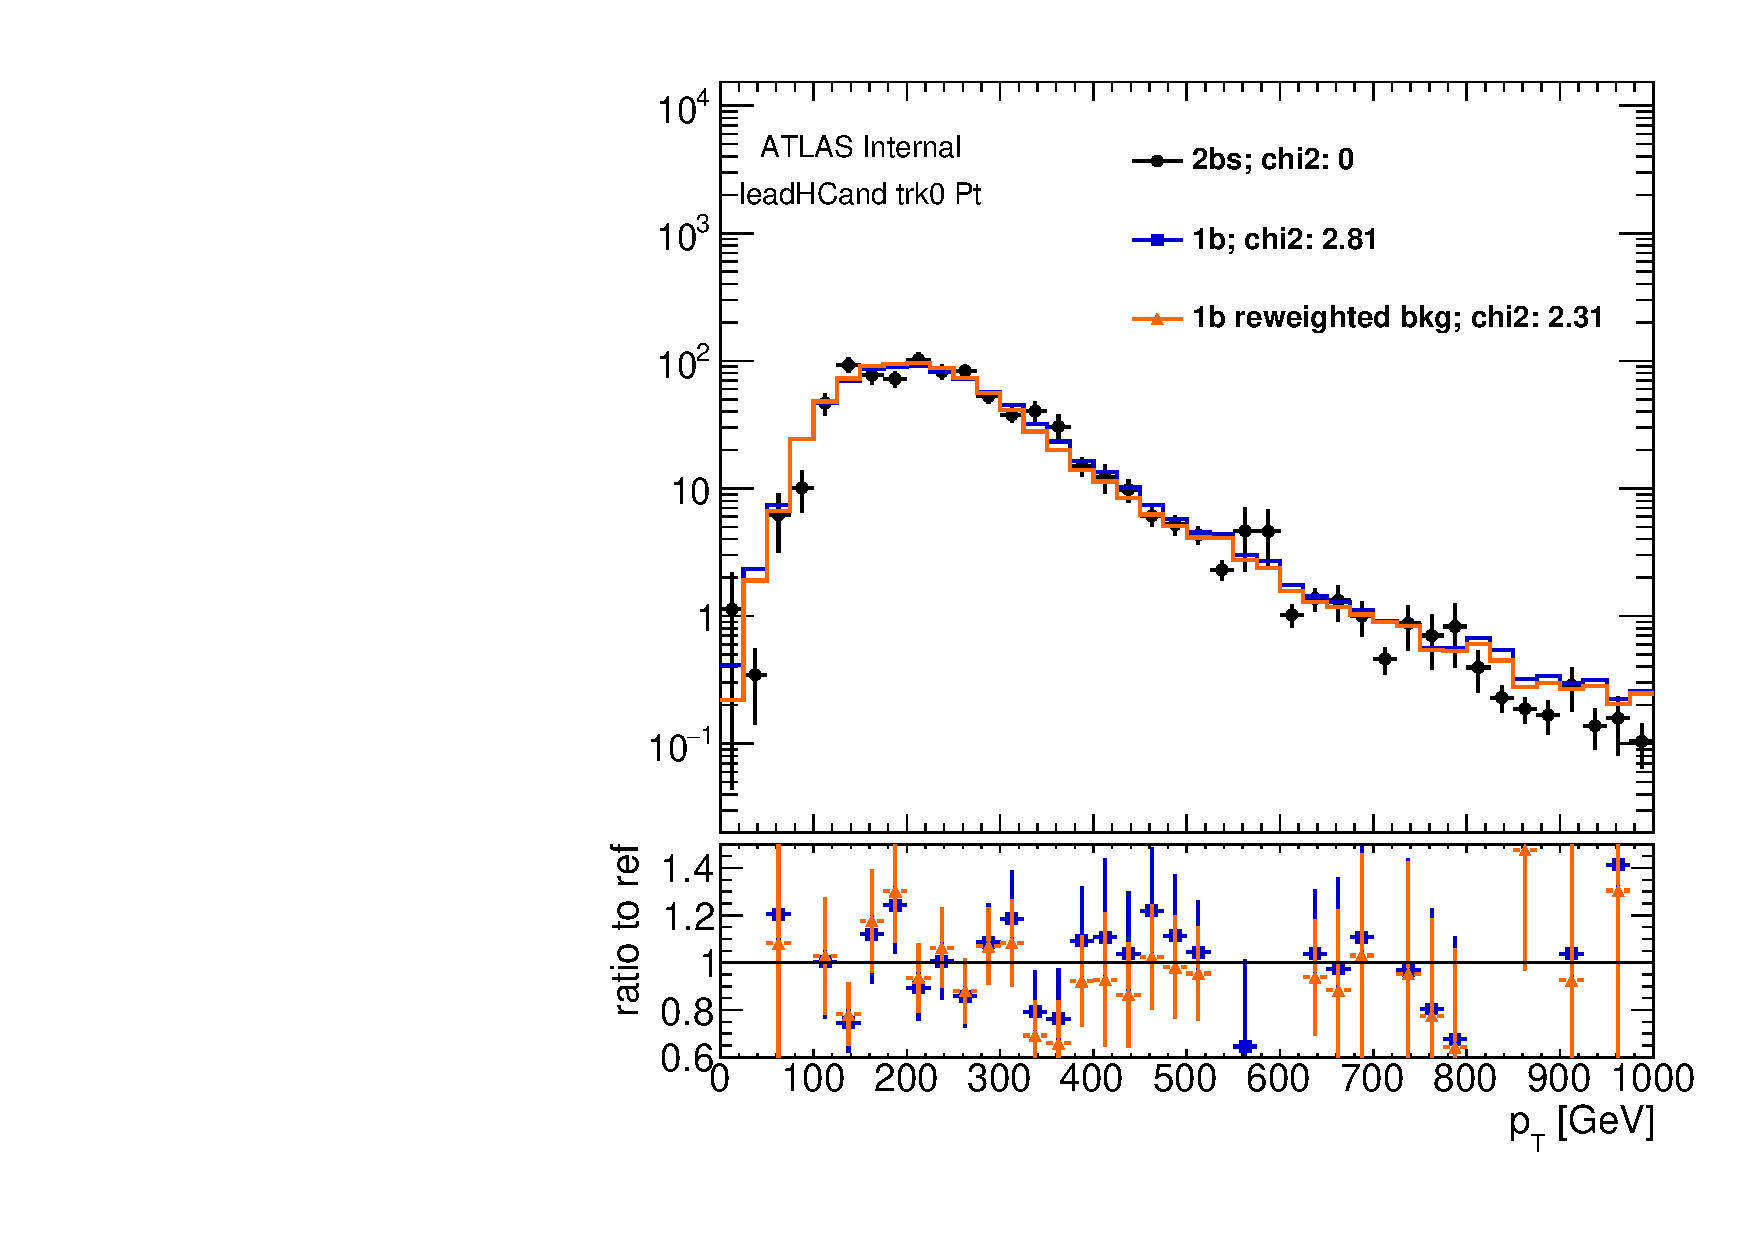
\includegraphics[width=0.48\textwidth,angle=-90]{figures/boosted/AppendixReweight/Compare/Dijet_Incl_directcompare_leadHCand_trk0_Pt_1.pdf}
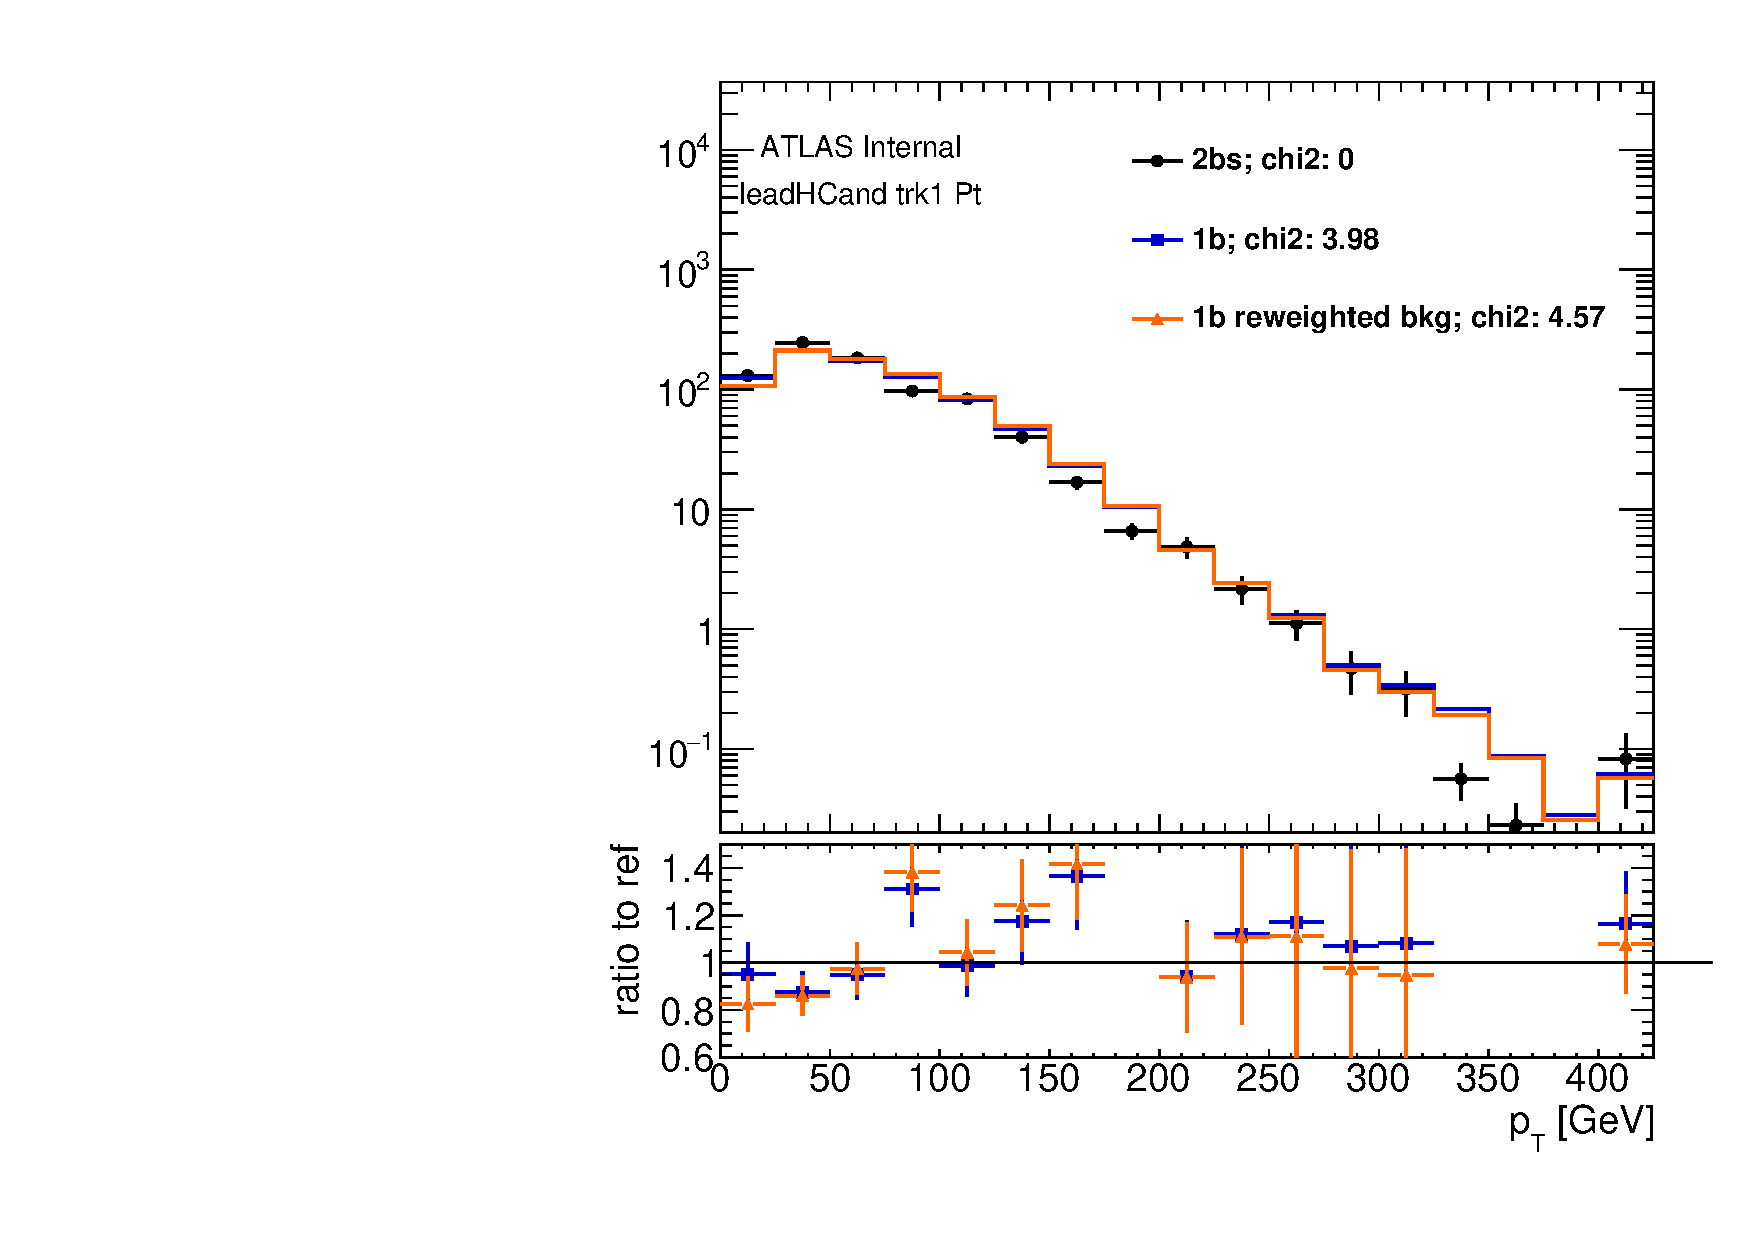
\includegraphics[width=0.48\textwidth,angle=-90]{figures/boosted/AppendixReweight/Compare/Dijet_Incl_directcompare_leadHCand_trk1_Pt_1.pdf}\\
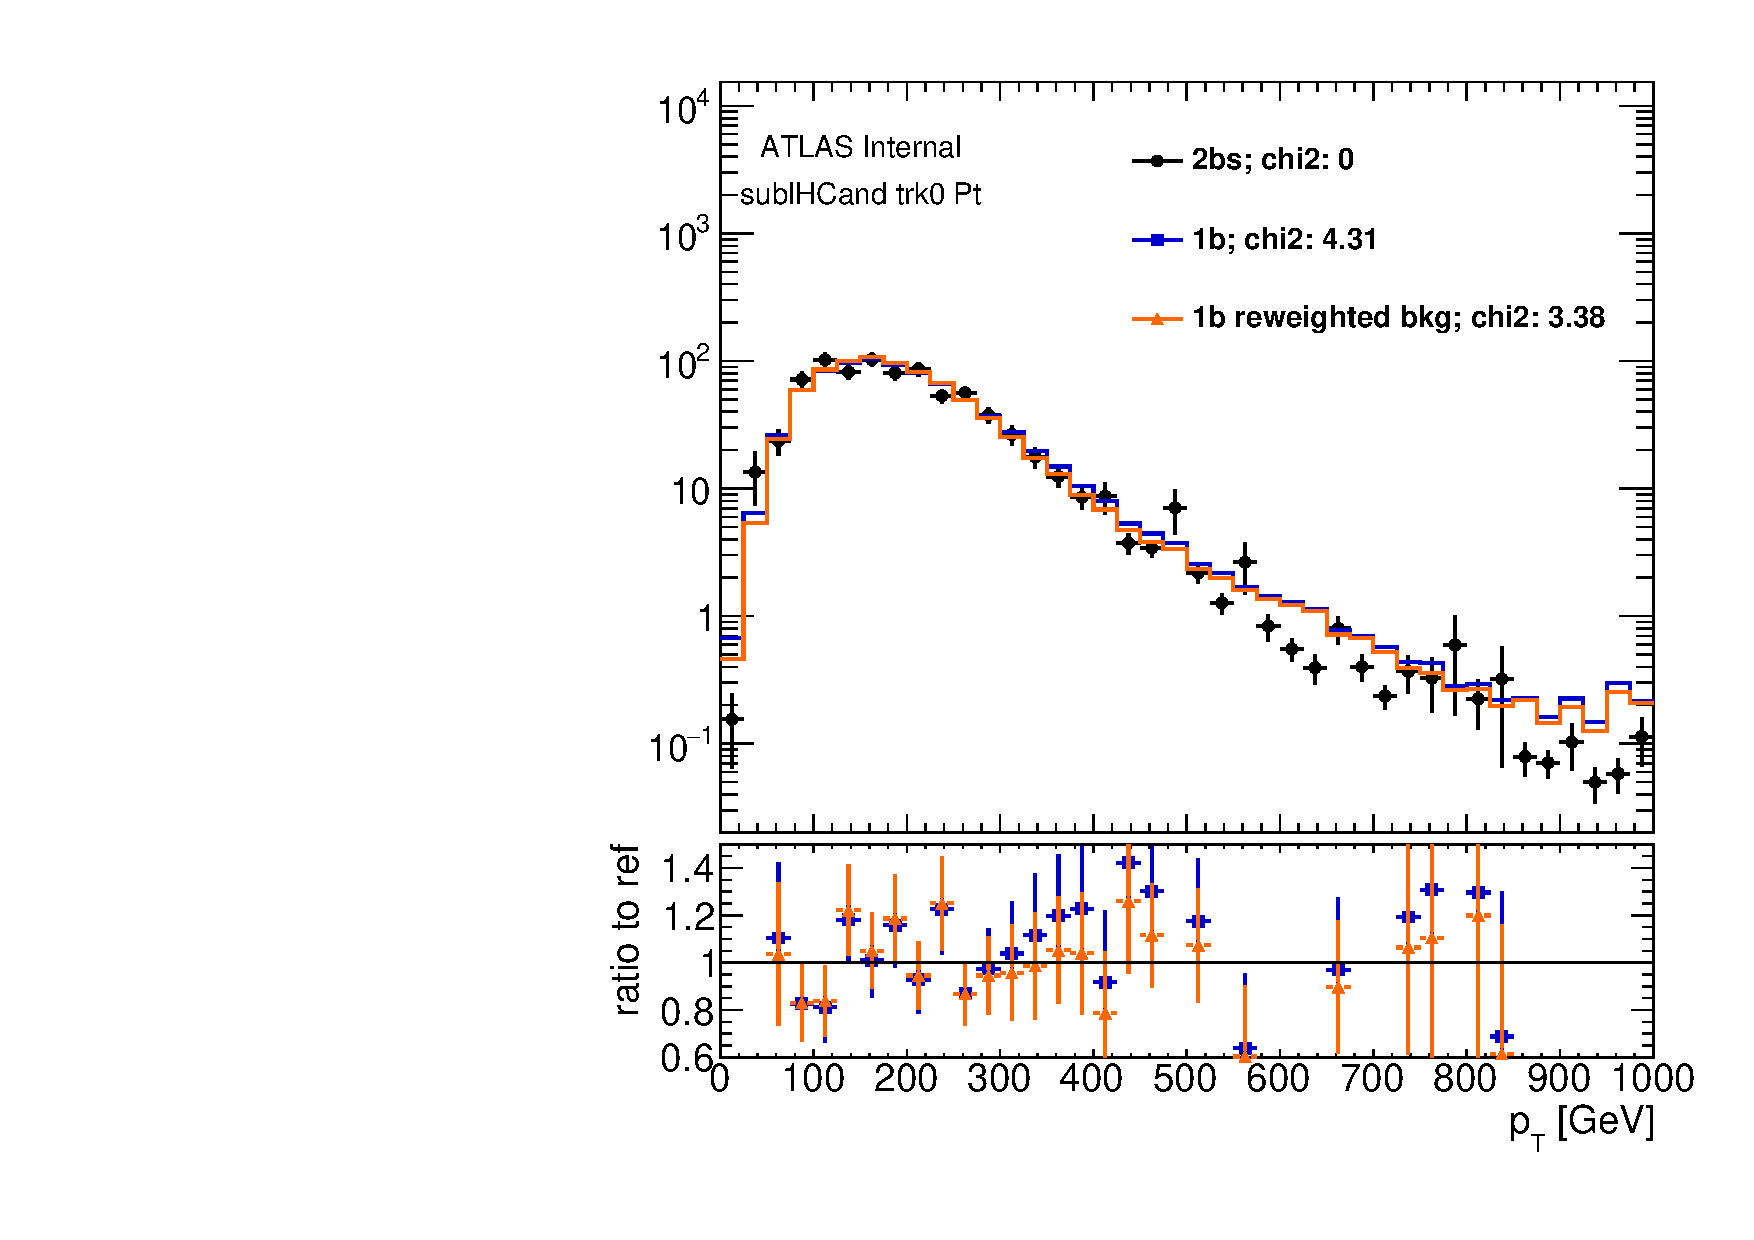
\includegraphics[width=0.48\textwidth,angle=-90]{figures/boosted/AppendixReweight/Compare/Dijet_Incl_directcompare_sublHCand_trk0_Pt_1.pdf}
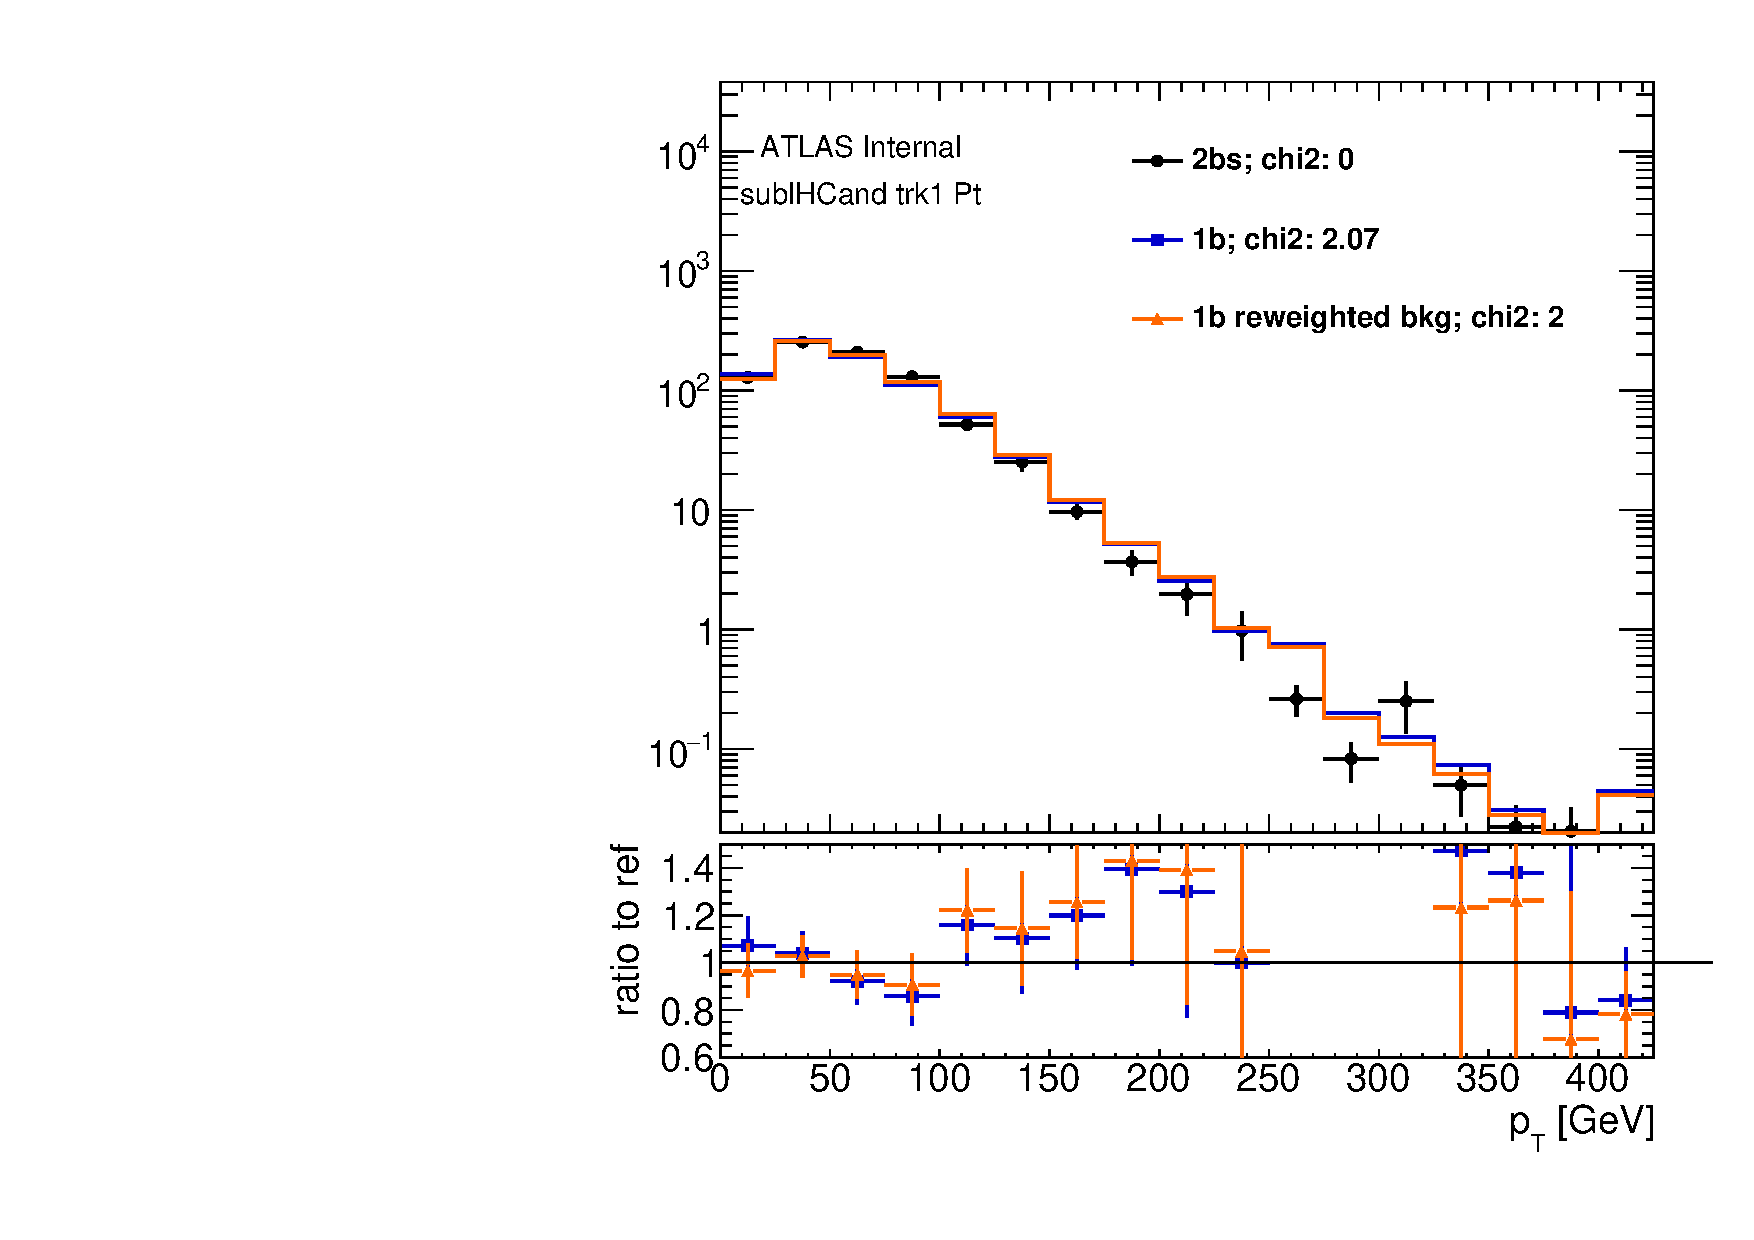
\includegraphics[width=0.48\textwidth,angle=-90]{figures/boosted/AppendixReweight/Compare/Dijet_Incl_directcompare_sublHCand_trk1_Pt_1.pdf}\\
\caption{Reweighted $2bs$ inclusive region predictions comaprison, for leading Higgs Candidate leading trackjet \pt (top left),  leading Higgs Candidate subleading trackjet \pt (top right), subleading Higgs Candidate leading trackjet \pt (bottom left), subleading Higgs Candidate subleading trackjet \pt (bottom right). $1b$ and reweighted $1b$ distributions are normalized to $2bs$.}
\label{fig:app-rw-comp-dijet-2bs-trkjet}
\end{center}
\end{figure*}

\begin{figure*}[htbp!]
\begin{center}
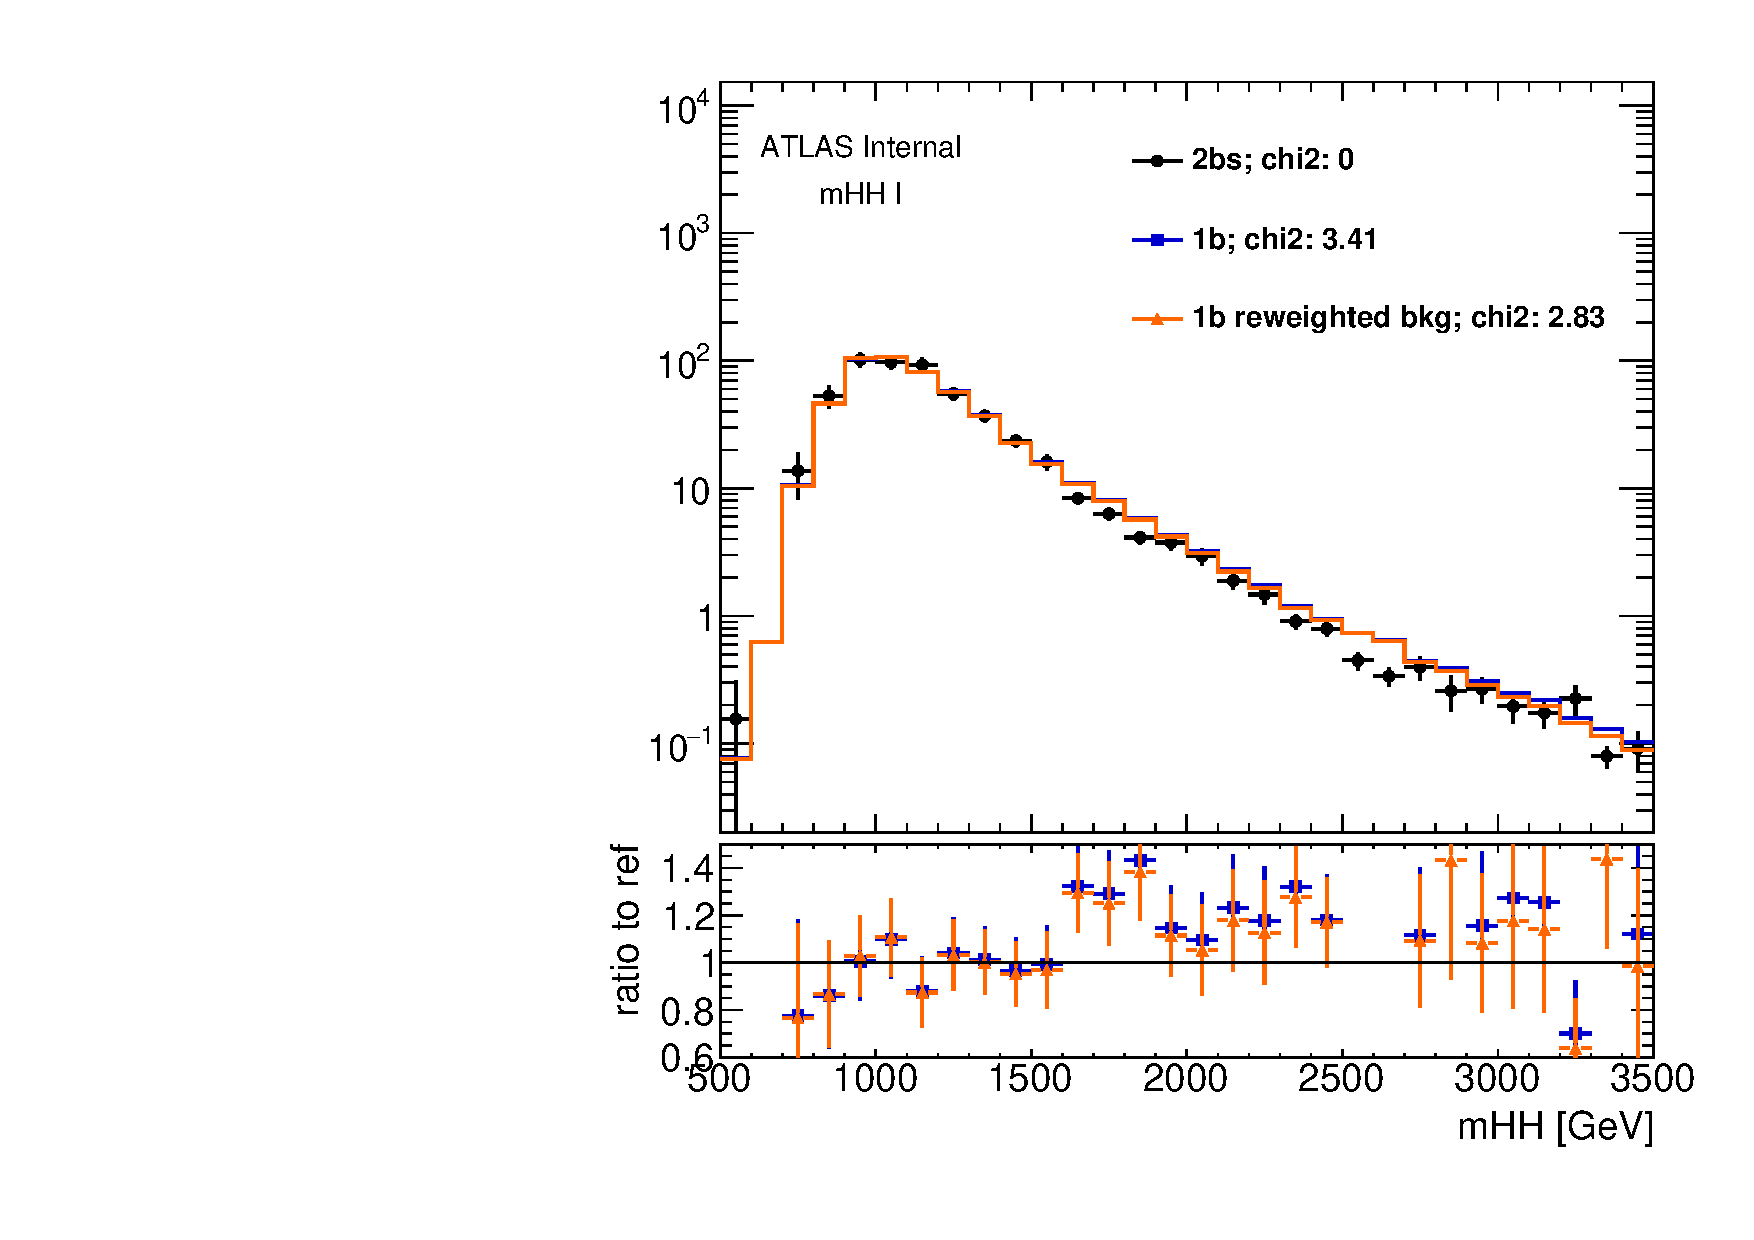
\includegraphics[width=0.4\textwidth,angle=-90]{figures/boosted/AppendixReweight/Compare/Dijet_Sideband_directcompare_mHH_l_1.pdf}\\
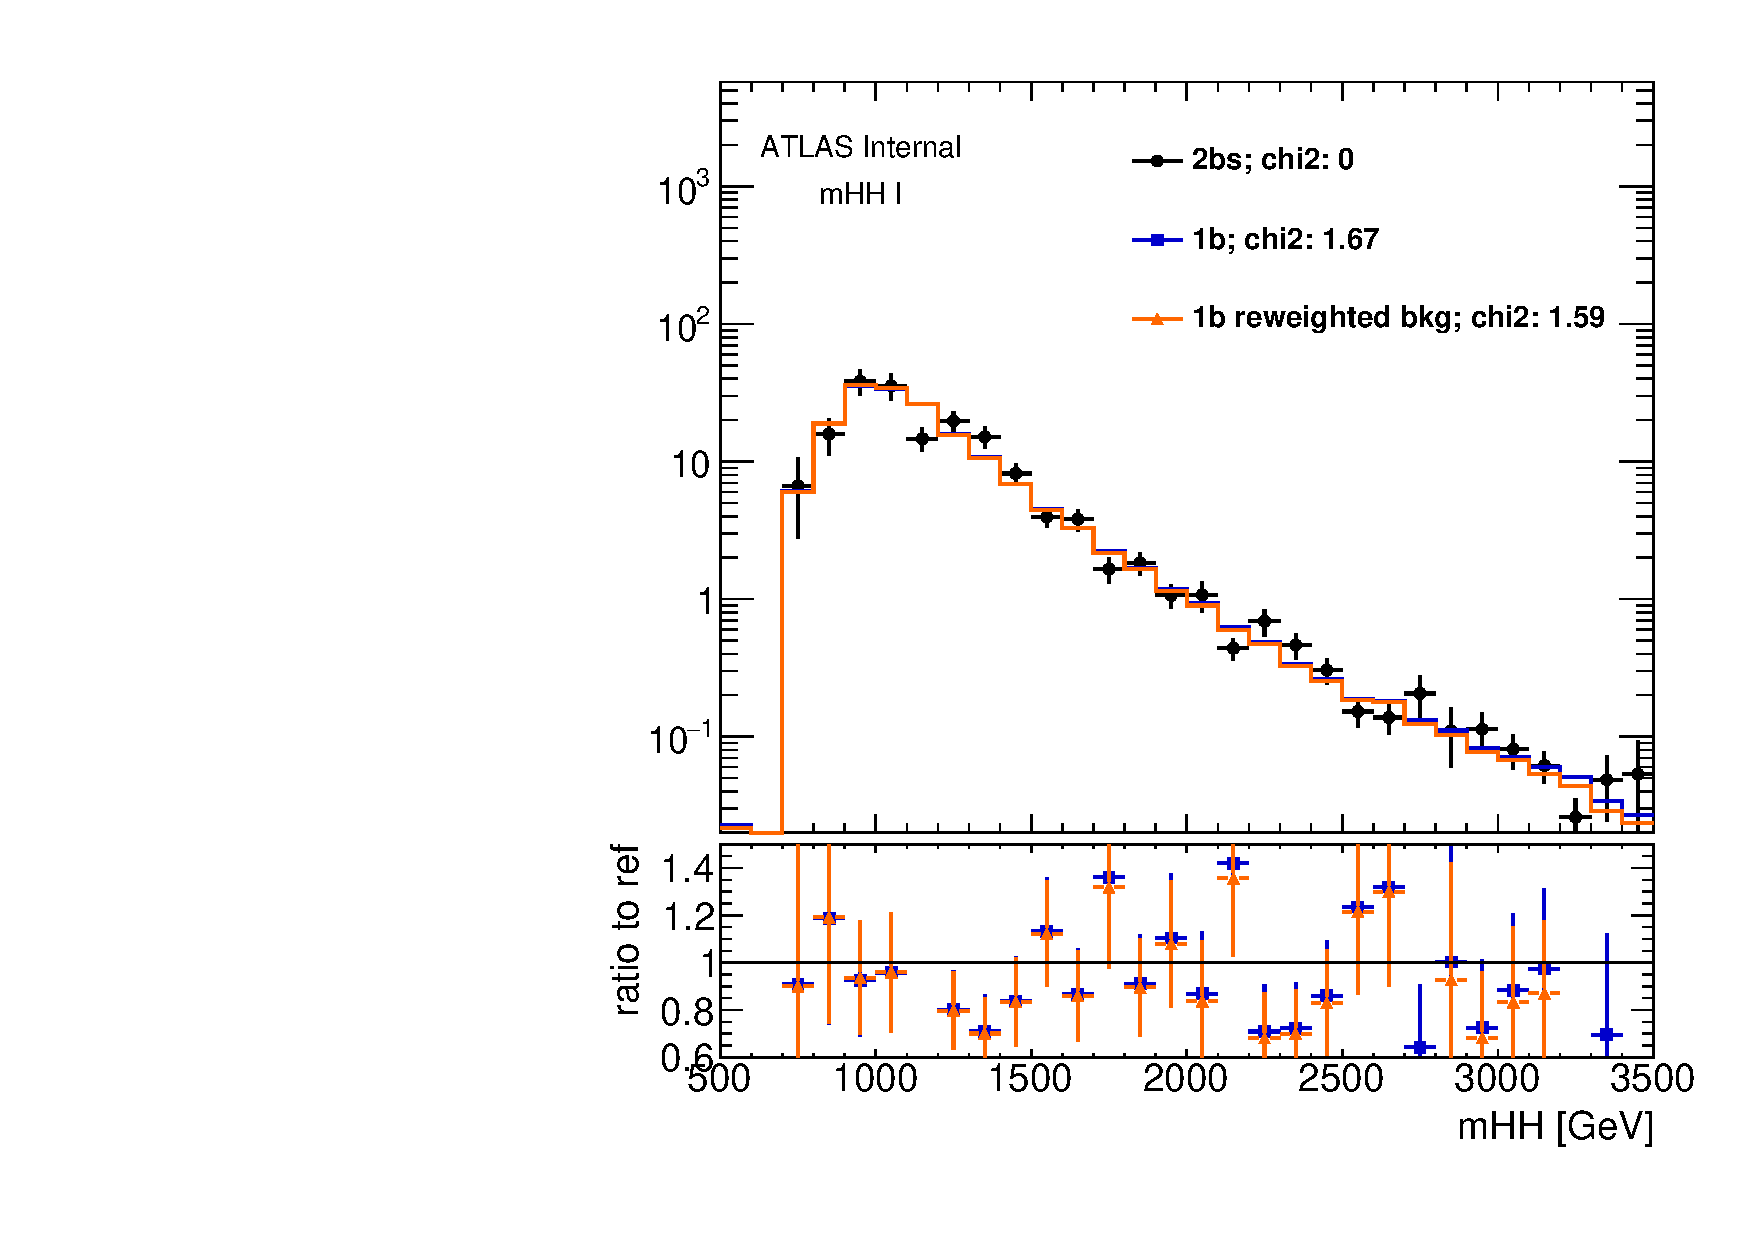
\includegraphics[width=0.4\textwidth,angle=-90]{figures/boosted/AppendixReweight/Compare/Dijet_Control_directcompare_mHH_l_1.pdf}\\
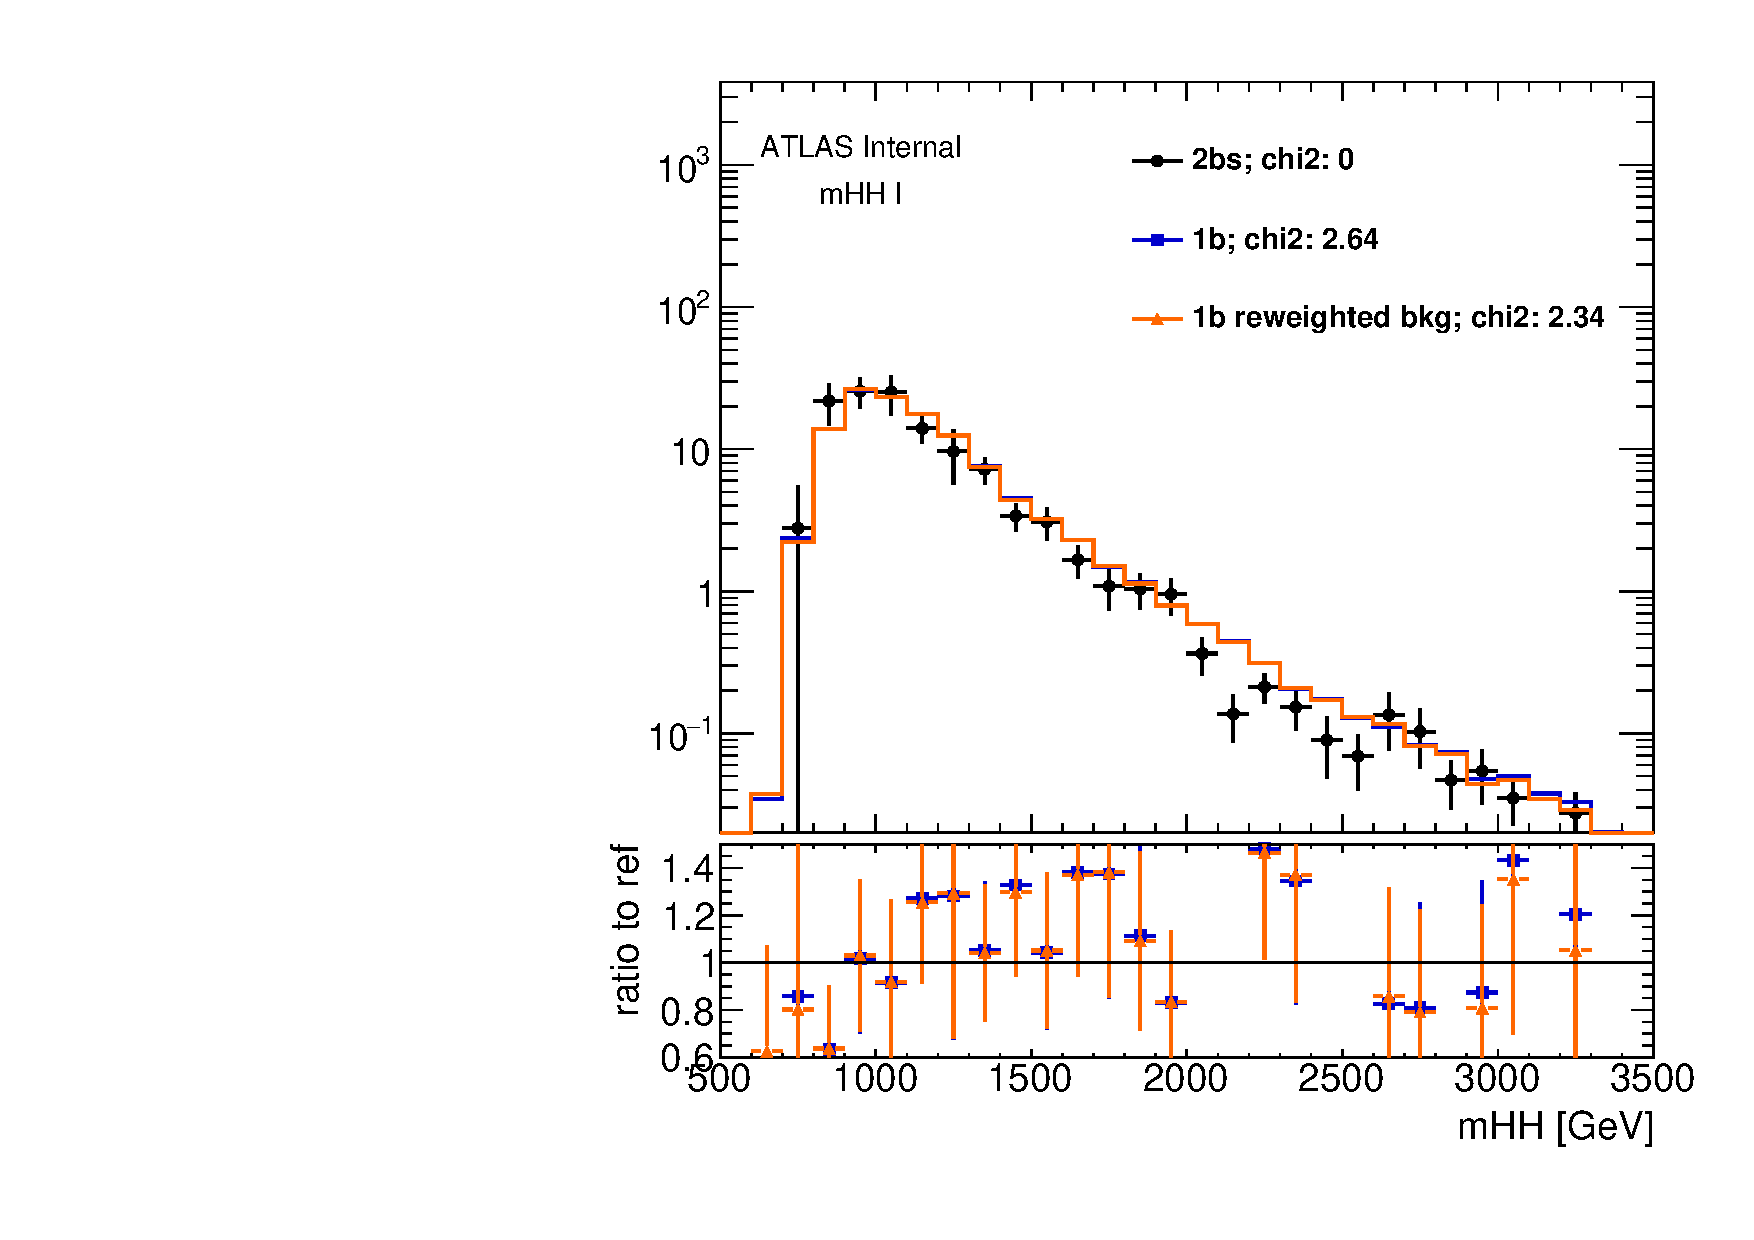
\includegraphics[width=0.4\textwidth,angle=-90]{figures/boosted/AppendixReweight/Compare/Dijet_Signal_directcompare_mHH_l_1.pdf}
\caption{Reweighted $2bs$ Sideband (top)/Control (middle)/Signal(bottom) region predictions comaprison, for MJJ. The Signal region is not blinded, since it is MC distribution. $1b$ and reweighted $1b$ distributions are normalized to $2bs$.}
\label{fig:app-rw-comp-dijet-2bs}
\end{center}
\end{figure*}

\begin{figure*}[htbp!]
\begin{center}
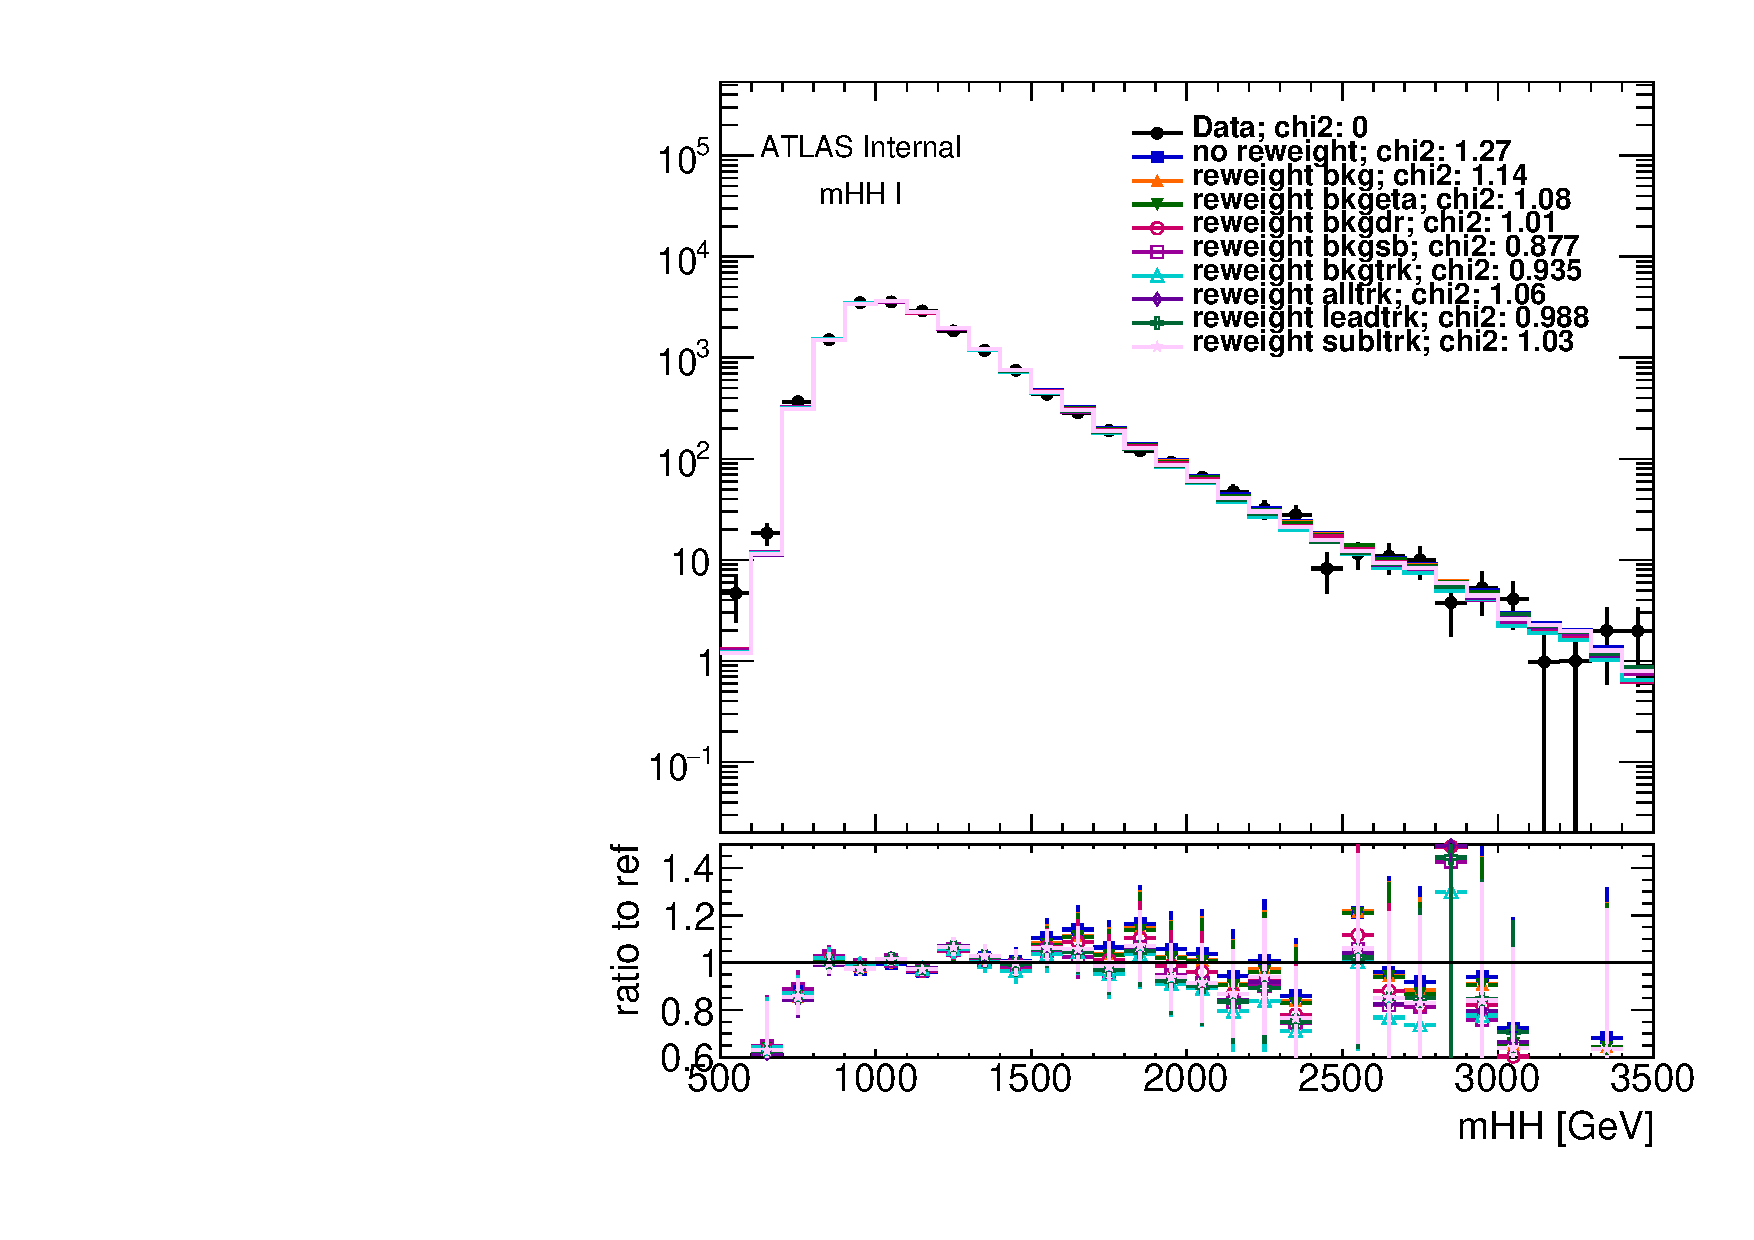
\includegraphics[width=0.4\textwidth,angle=-90]{figures/boosted/AppendixReweight/Compare/Data_TwoTag_split_Sideband_directcompare_mHH_l_1.pdf}\\
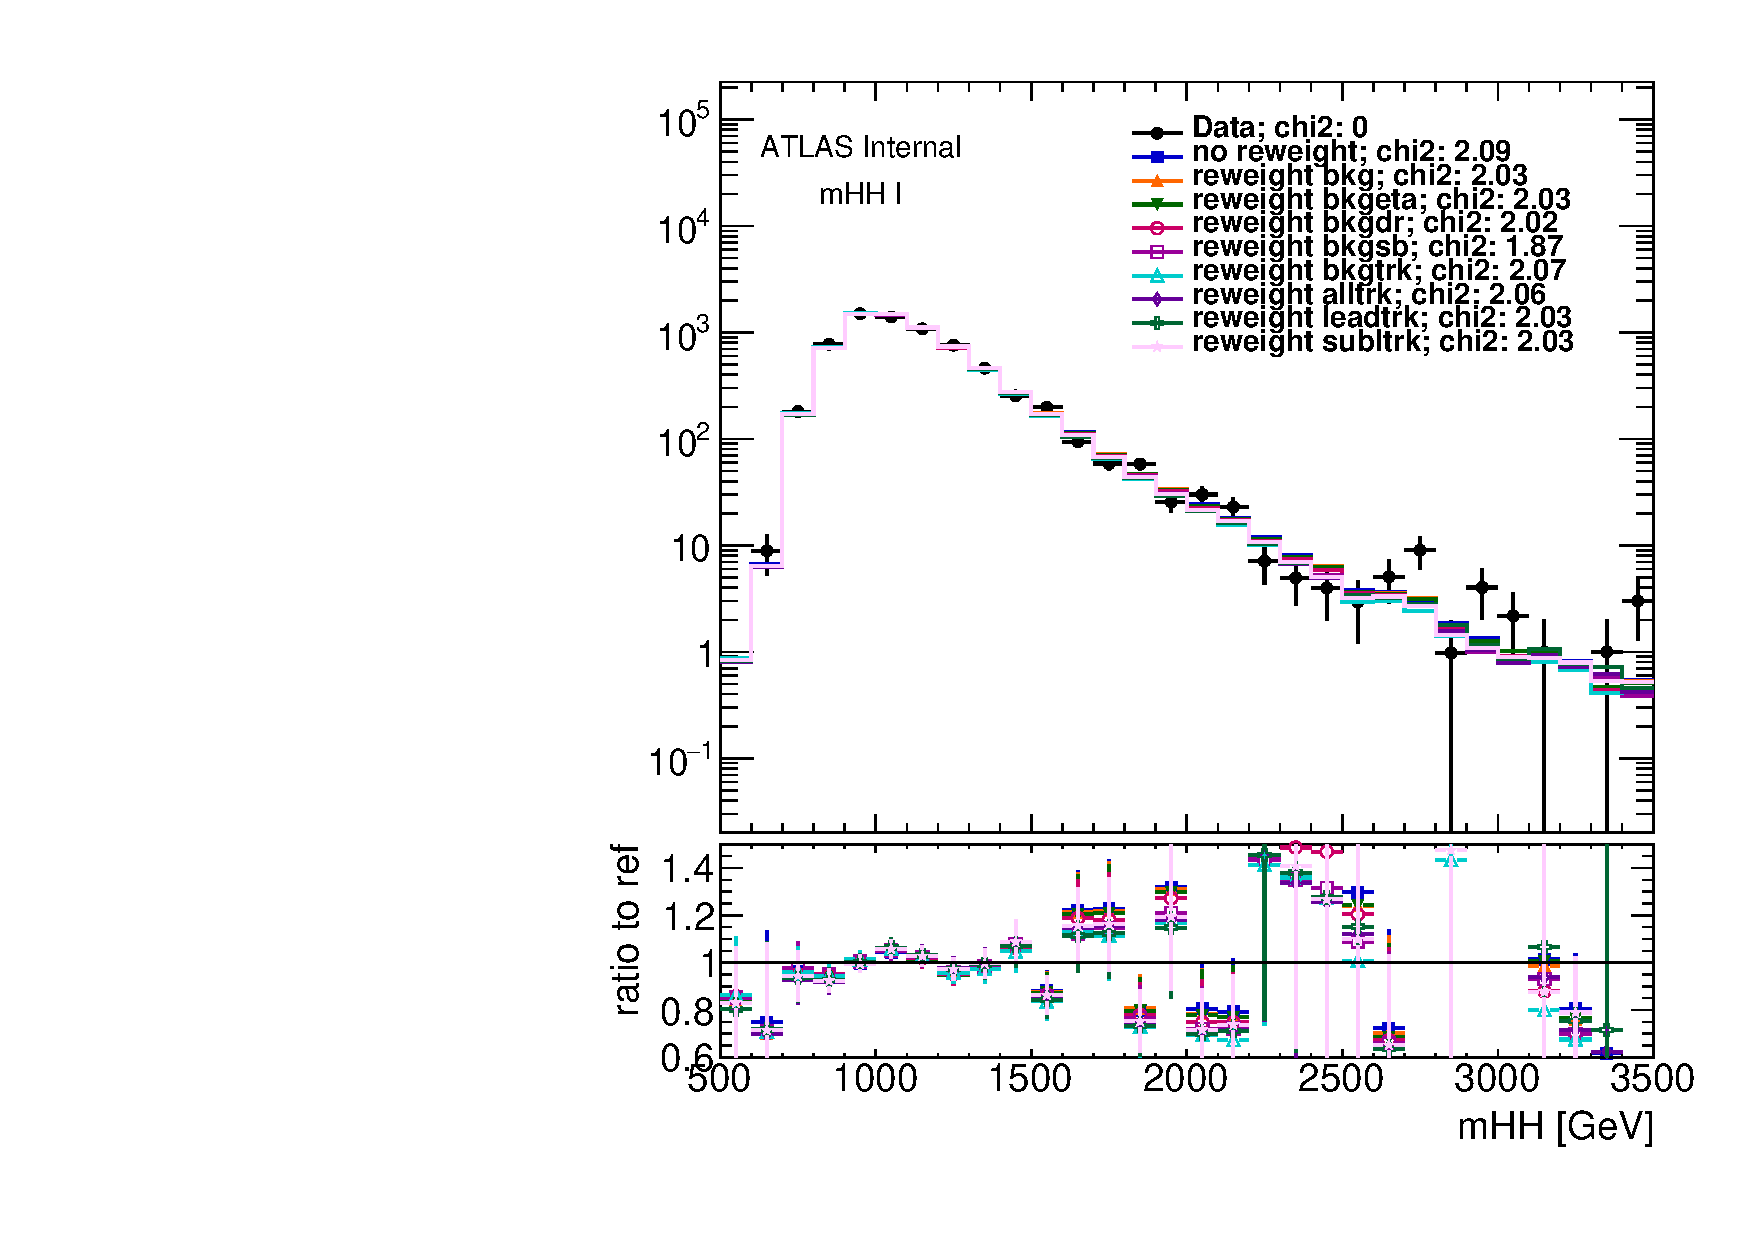
\includegraphics[width=0.4\textwidth,angle=-90]{figures/boosted/AppendixReweight/Compare/Data_TwoTag_split_Control_directcompare_mHH_l_1.pdf}\\
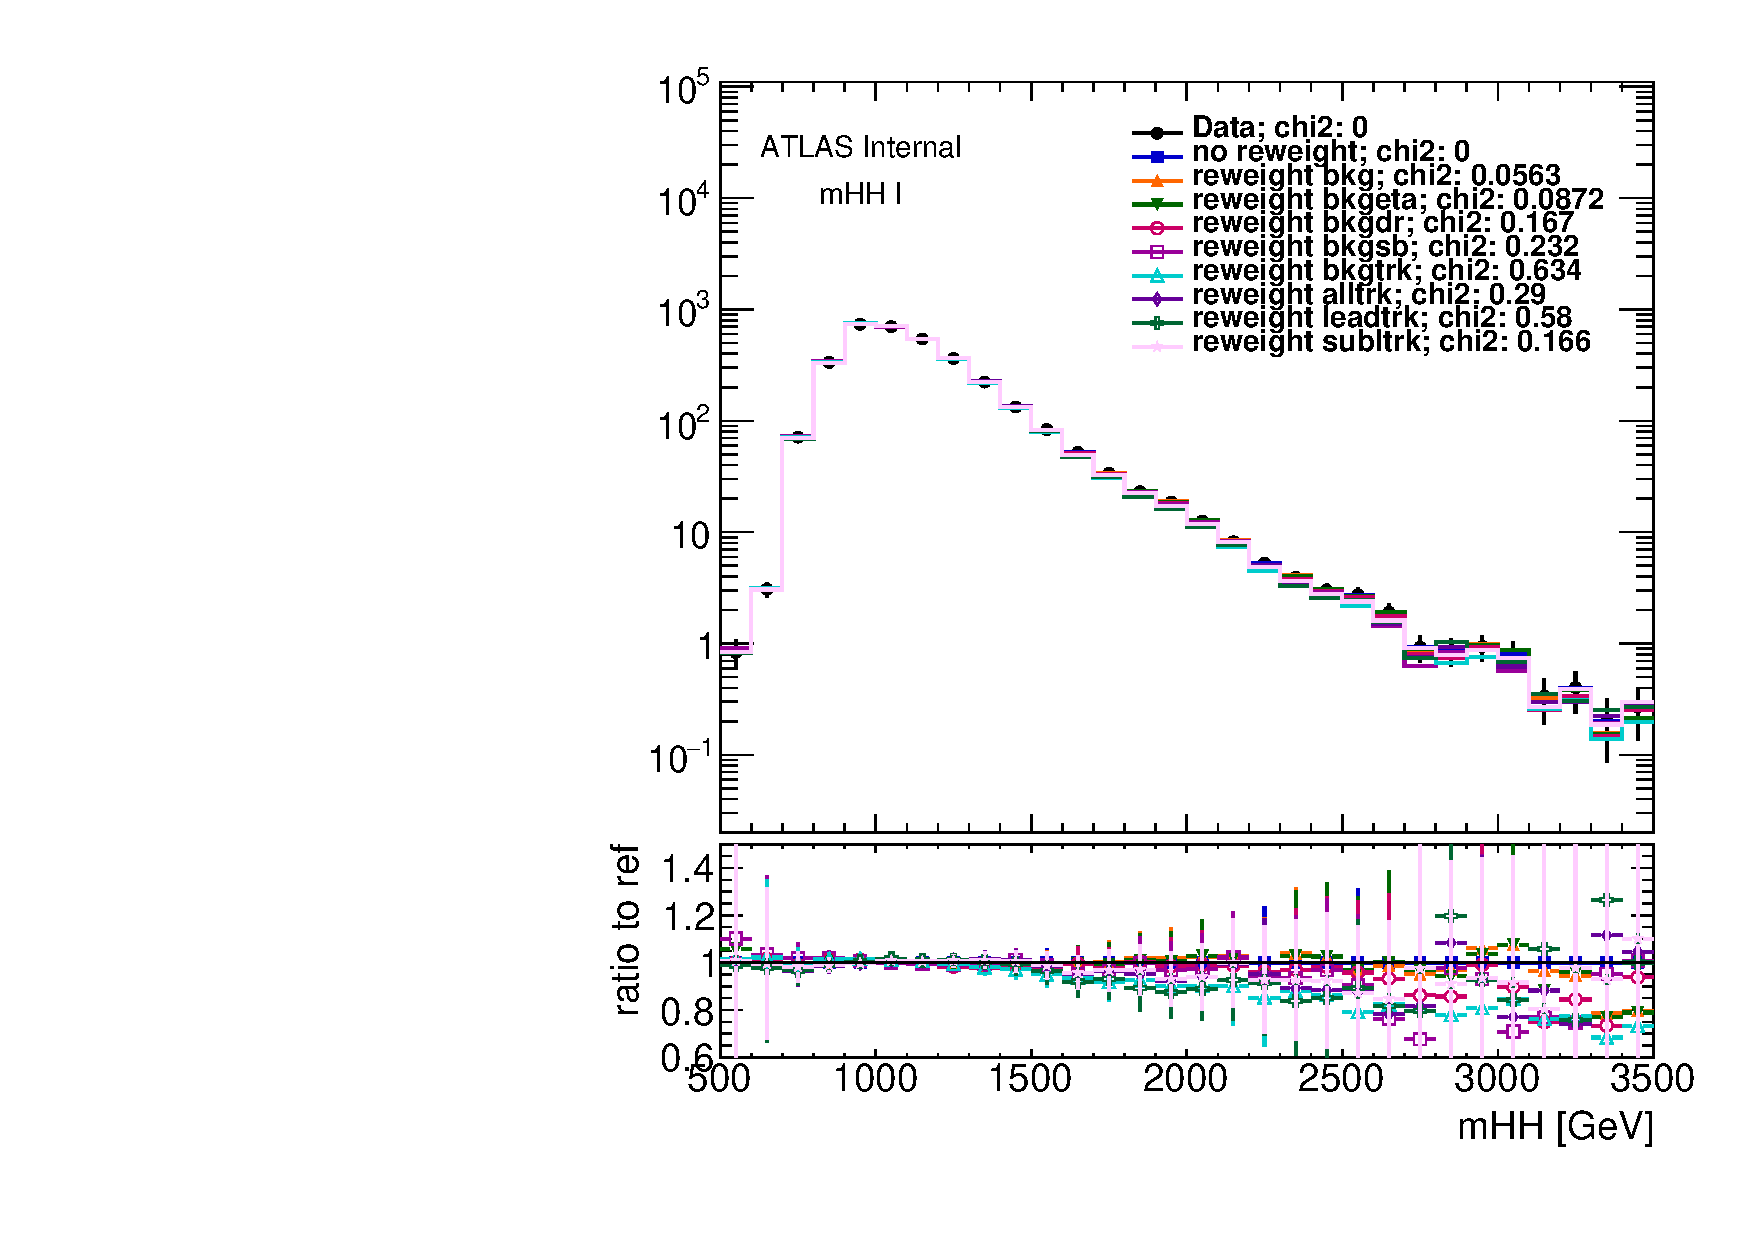
\includegraphics[width=0.4\textwidth,angle=-90]{figures/boosted/AppendixReweight/Compare/Data_TwoTag_split_Signal_directcompare_mHH_l_1.pdf}
\caption{Reweighted $2bs$ Sideband (top)/Control (middle)/Signal(bottom) region predictions comaprison, for MJJ. The Signal region is blinded, where the distribution is replaced with the non-reweighted distributions.}
\label{fig:app-rw-comp-2bs}
\end{center}
\end{figure*}

\begin{figure*}[htbp!]
\begin{center}
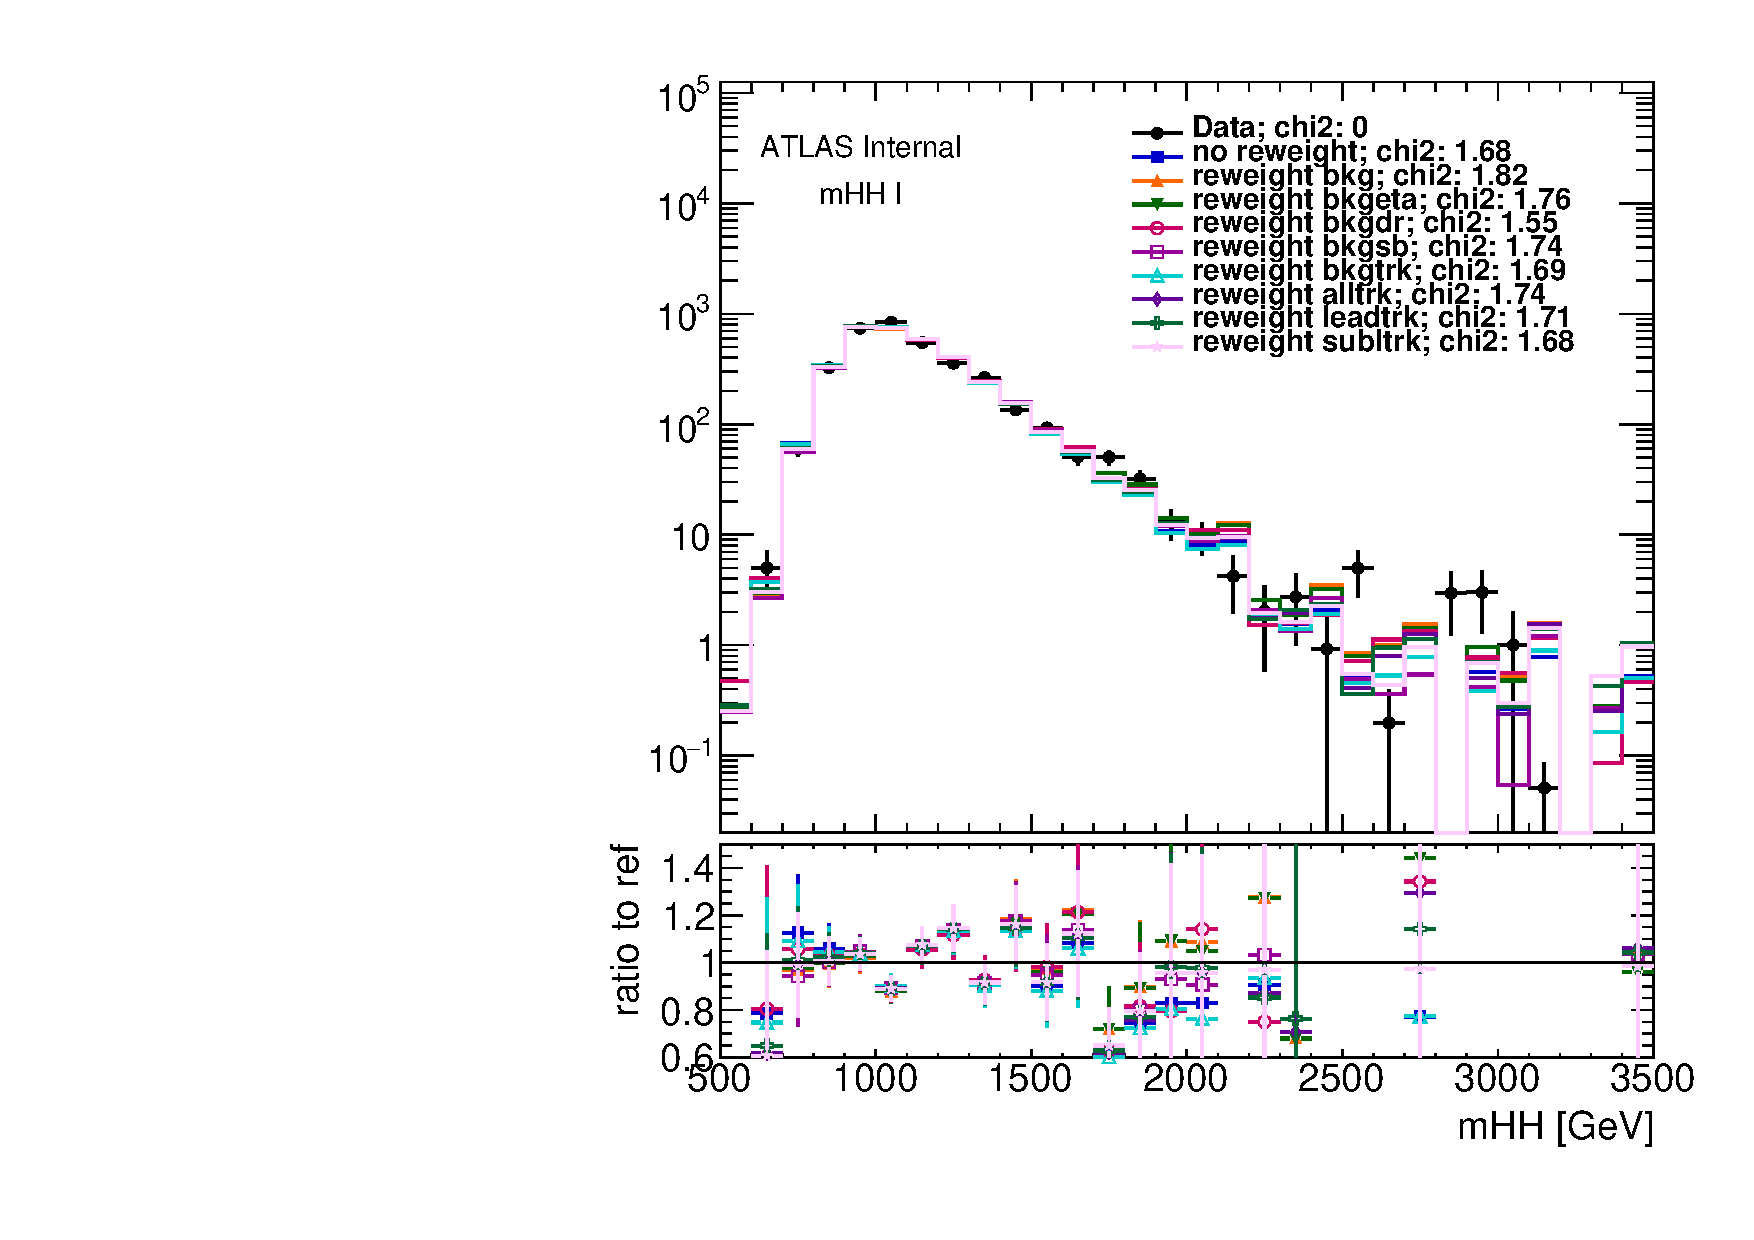
\includegraphics[width=0.4\textwidth,angle=-90]{figures/boosted/AppendixReweight/Compare/Data_ThreeTag_Sideband_directcompare_mHH_l_1.pdf}\\
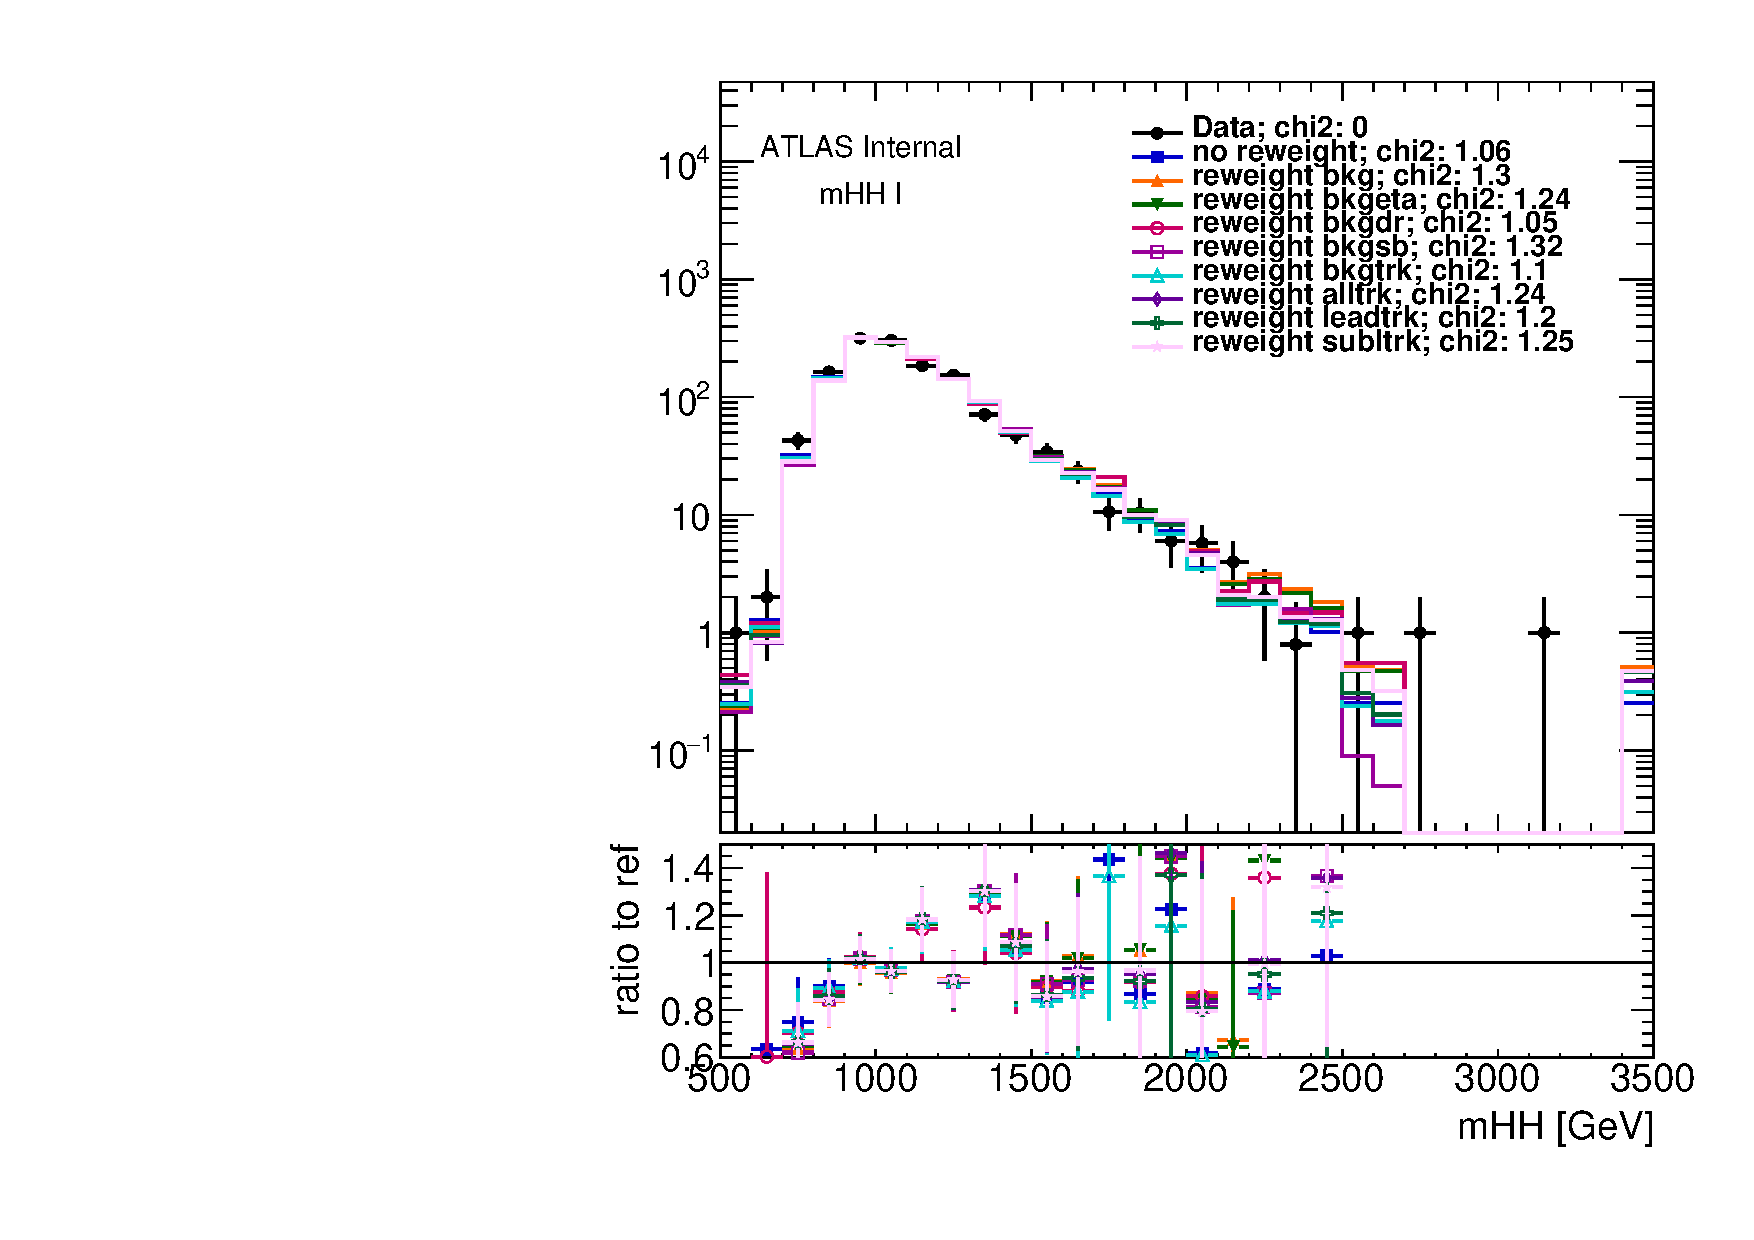
\includegraphics[width=0.4\textwidth,angle=-90]{figures/boosted/AppendixReweight/Compare/Data_ThreeTag_Control_directcompare_mHH_l_1.pdf}\\
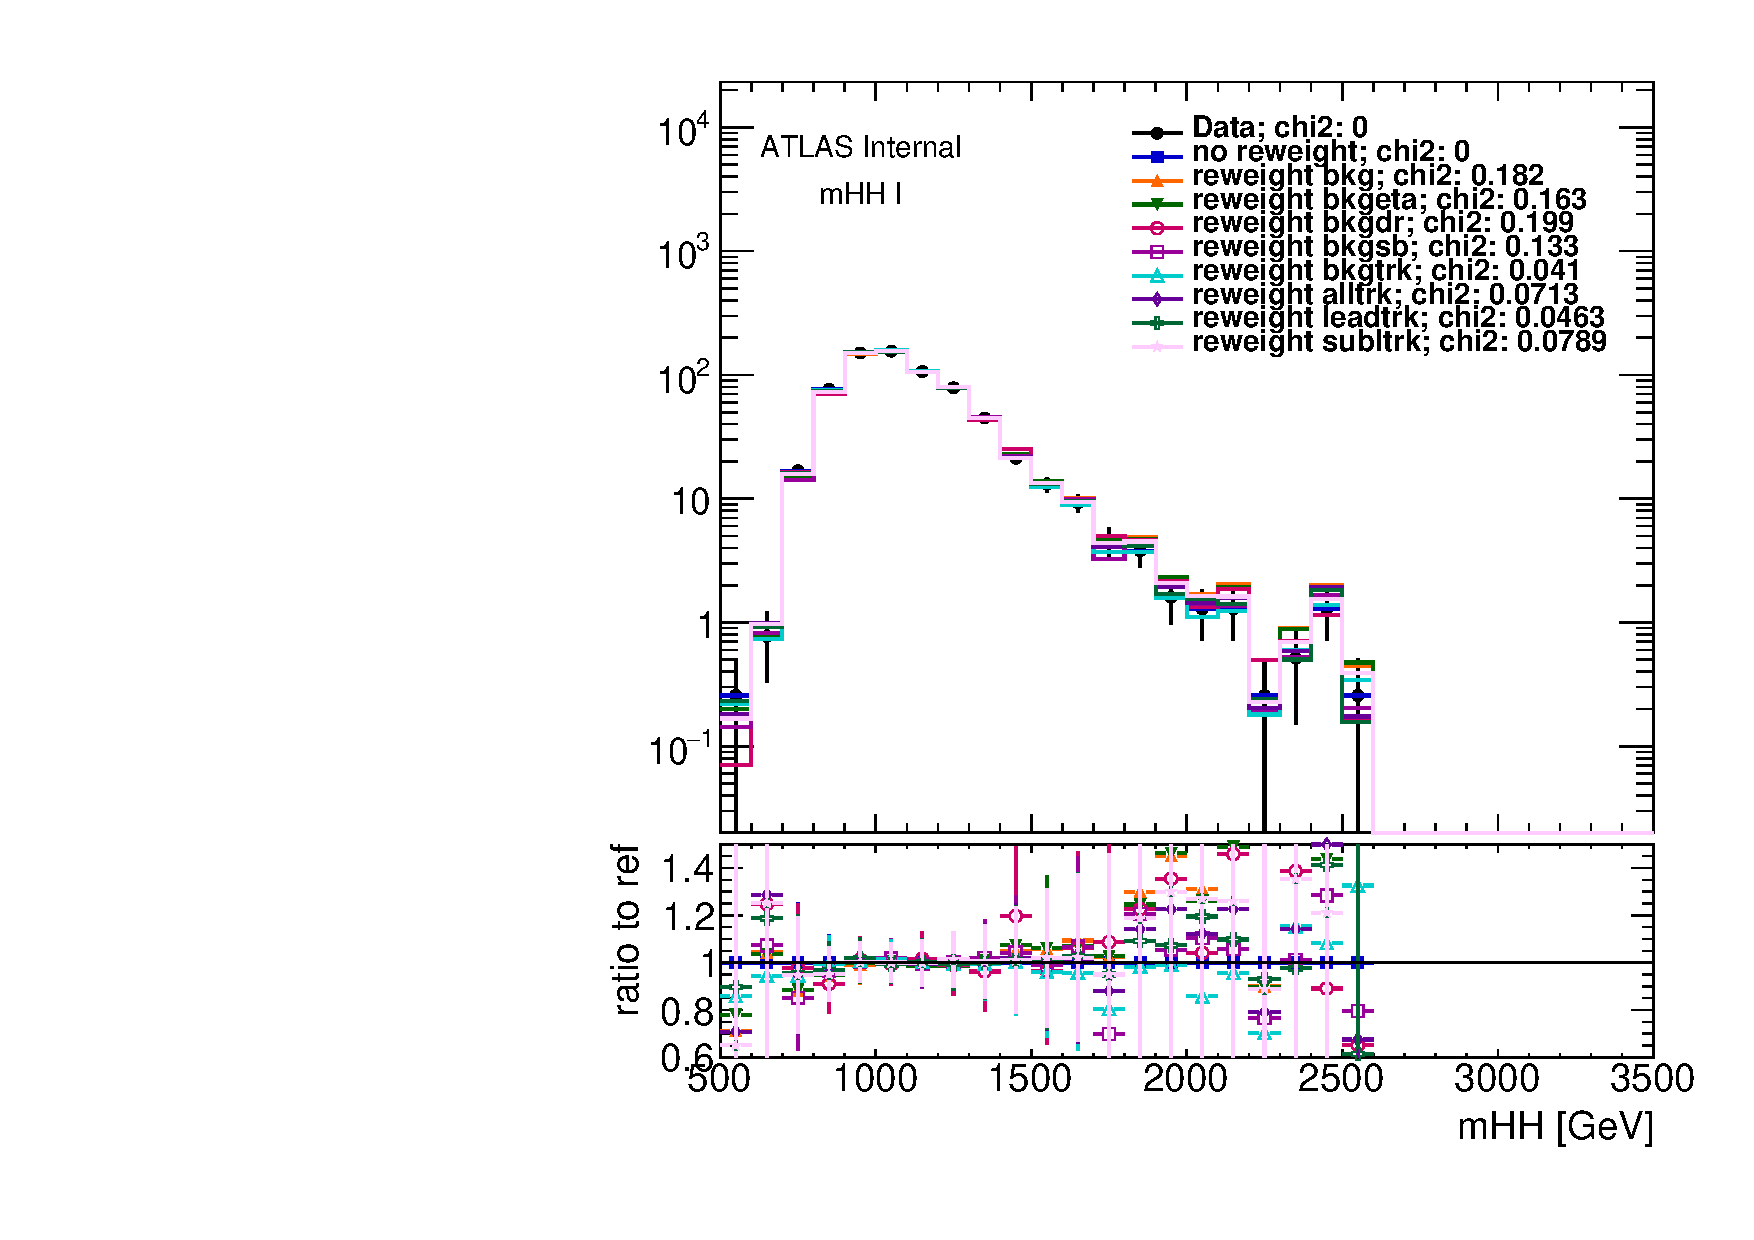
\includegraphics[width=0.4\textwidth,angle=-90]{figures/boosted/AppendixReweight/Compare/Data_ThreeTag_Signal_directcompare_mHH_l_1.pdf}
\caption{Reweighted $3b$ Sideband (top)/Control (middle)/Signal(bottom) region predictions comaprison, for MJJ. The Signal region is blinded, where the distribution is replaced with the non-reweighted distributions.}
\label{fig:app-rw-comp-3b}
\end{center}
\end{figure*}

\begin{figure*}[htbp!]
\begin{center}
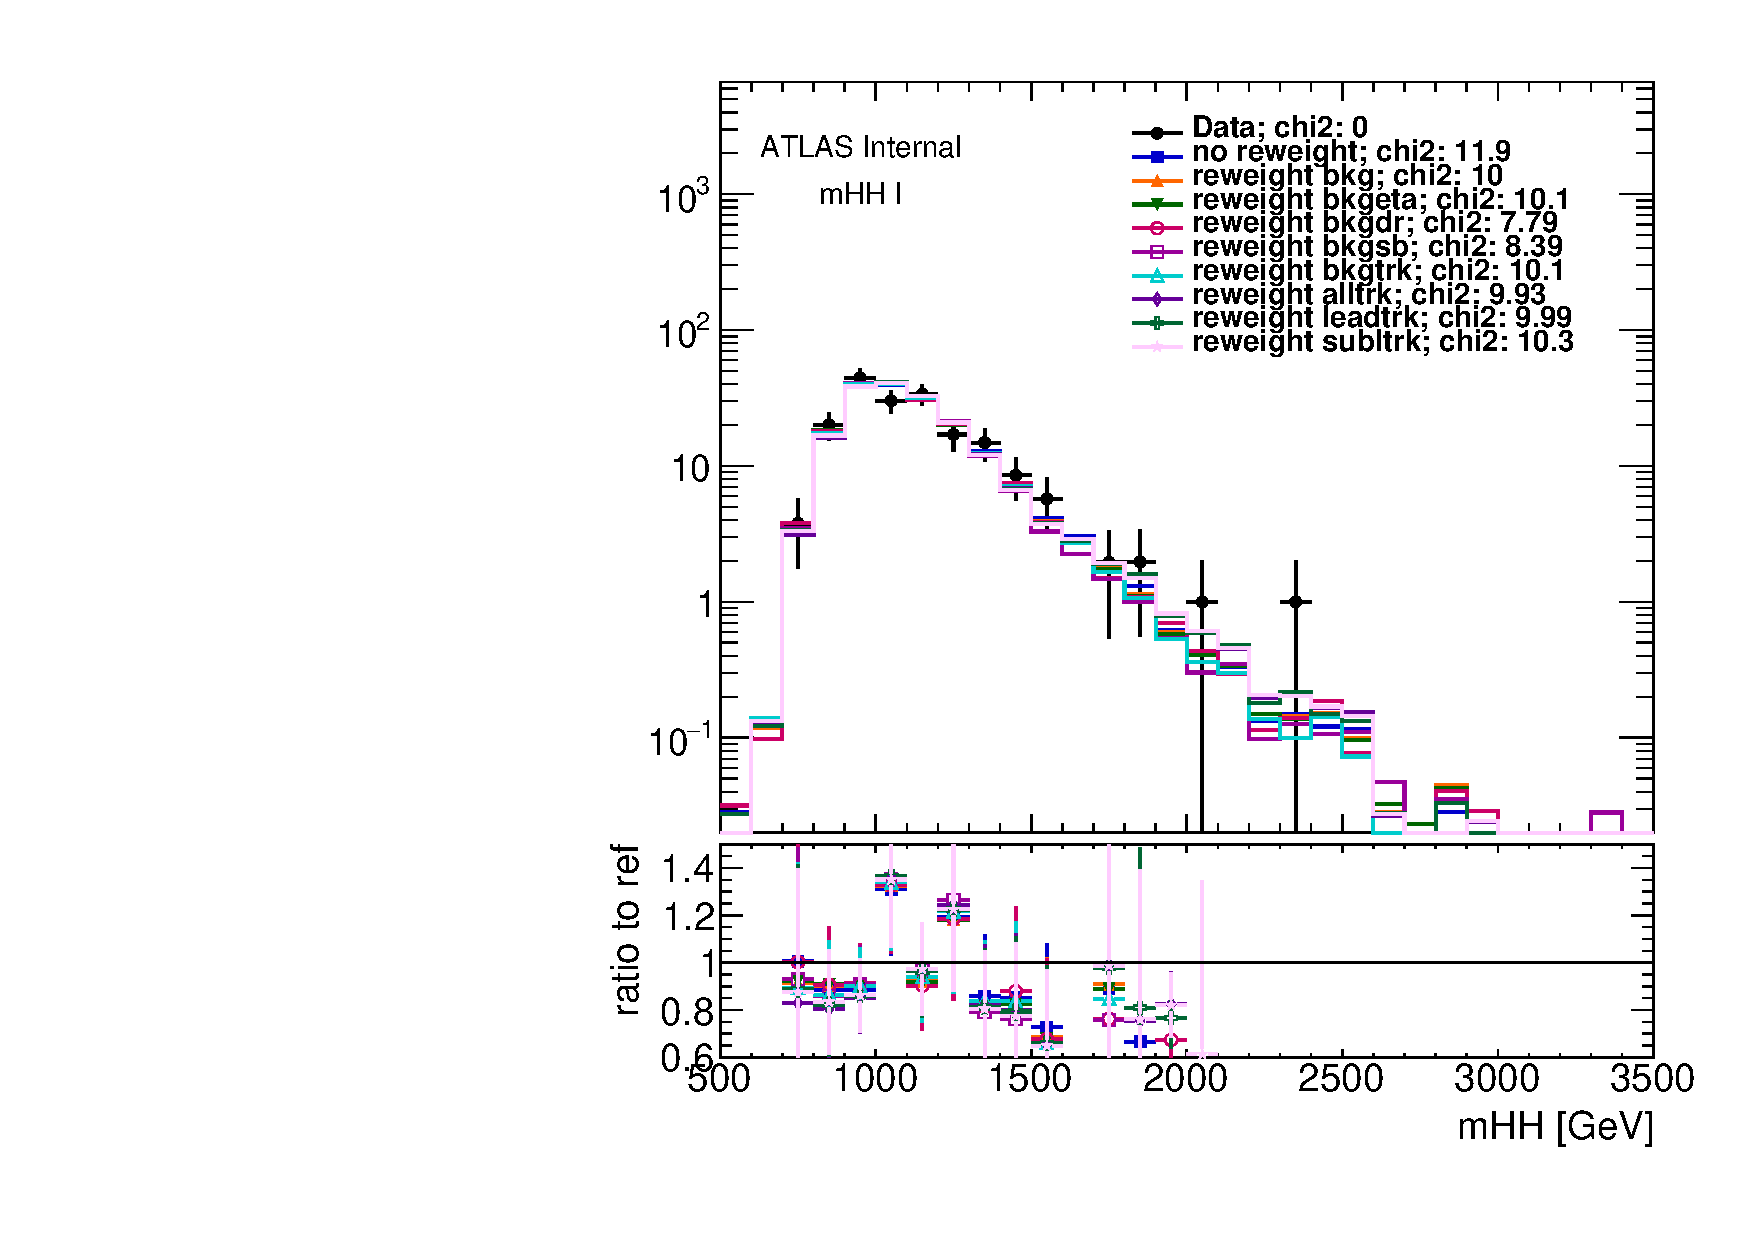
\includegraphics[width=0.4\textwidth,angle=-90]{figures/boosted/AppendixReweight/Compare/Data_FourTag_Sideband_directcompare_mHH_l_1.pdf}\\
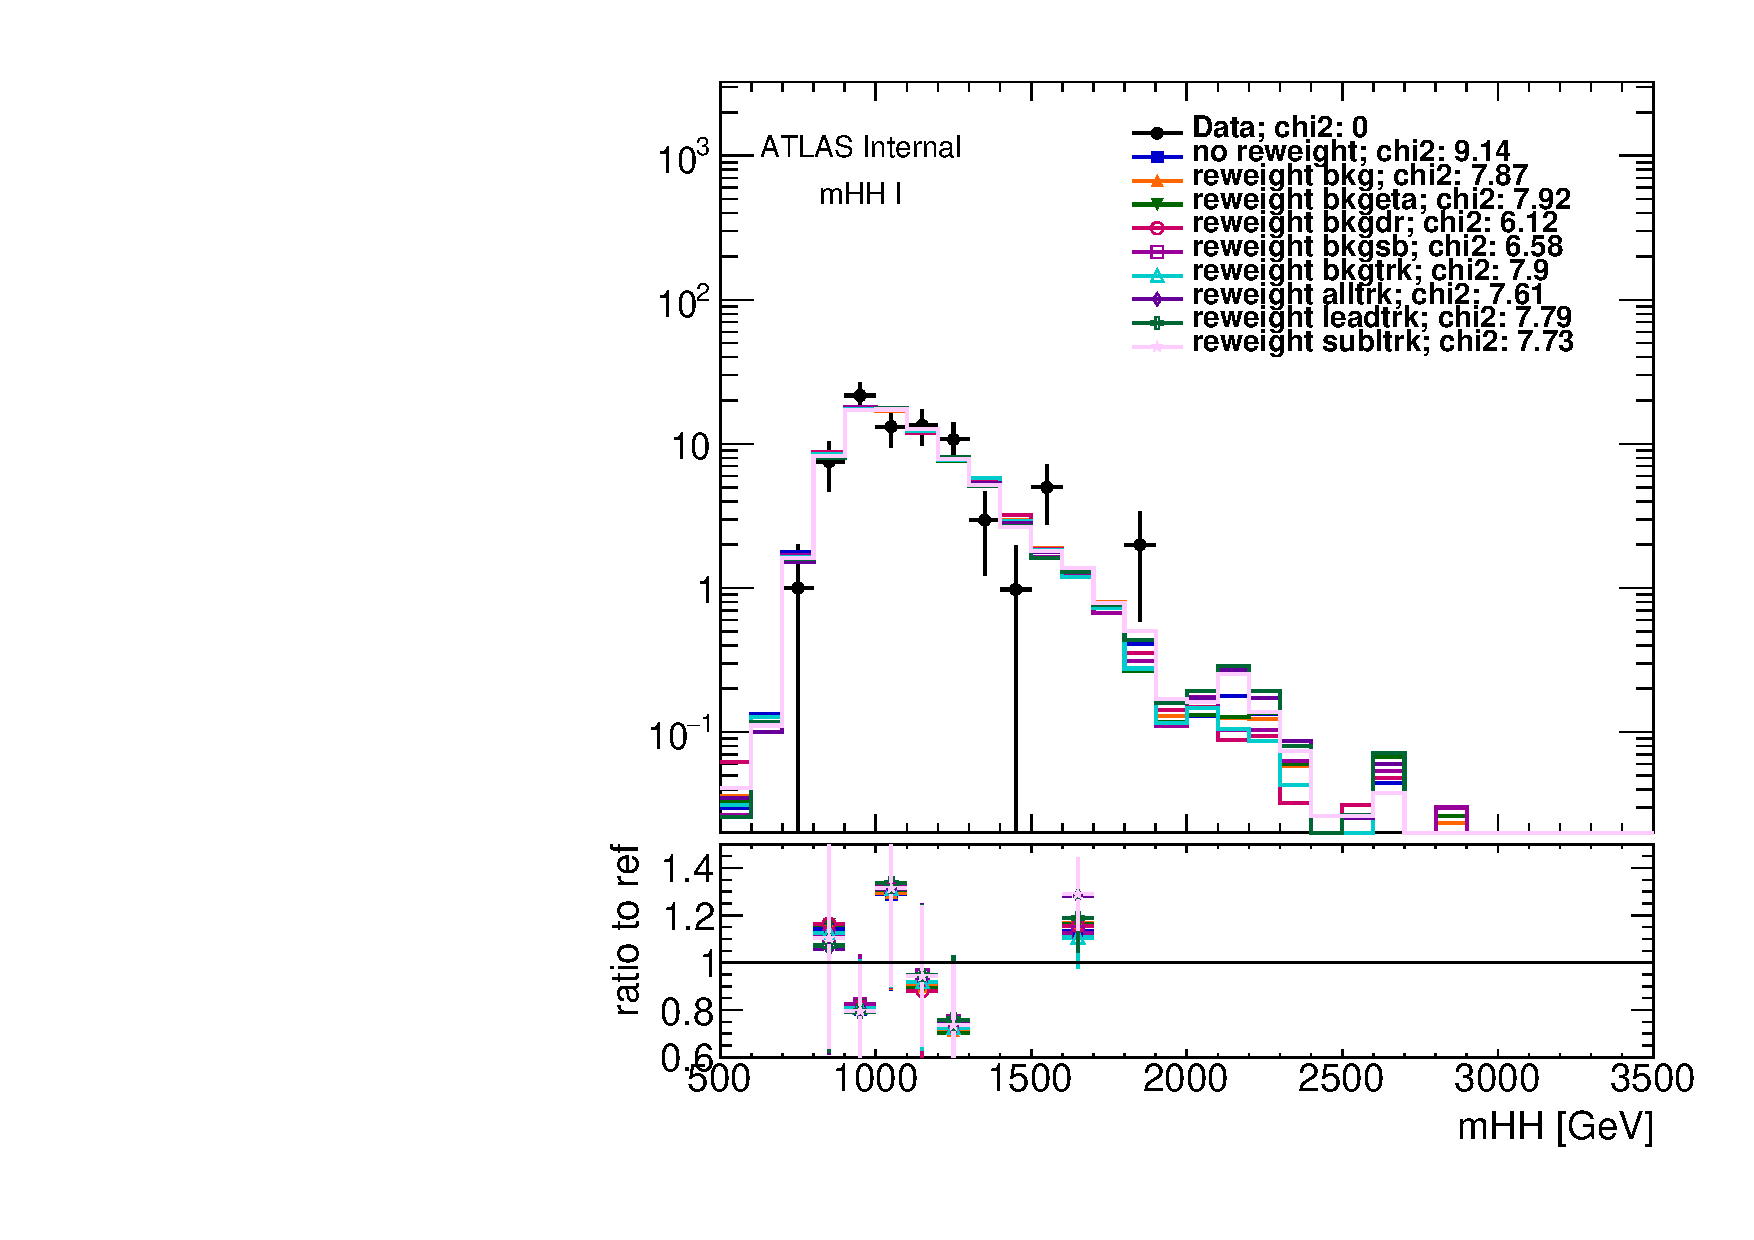
\includegraphics[width=0.4\textwidth,angle=-90]{figures/boosted/AppendixReweight/Compare/Data_FourTag_Control_directcompare_mHH_l_1.pdf}\\
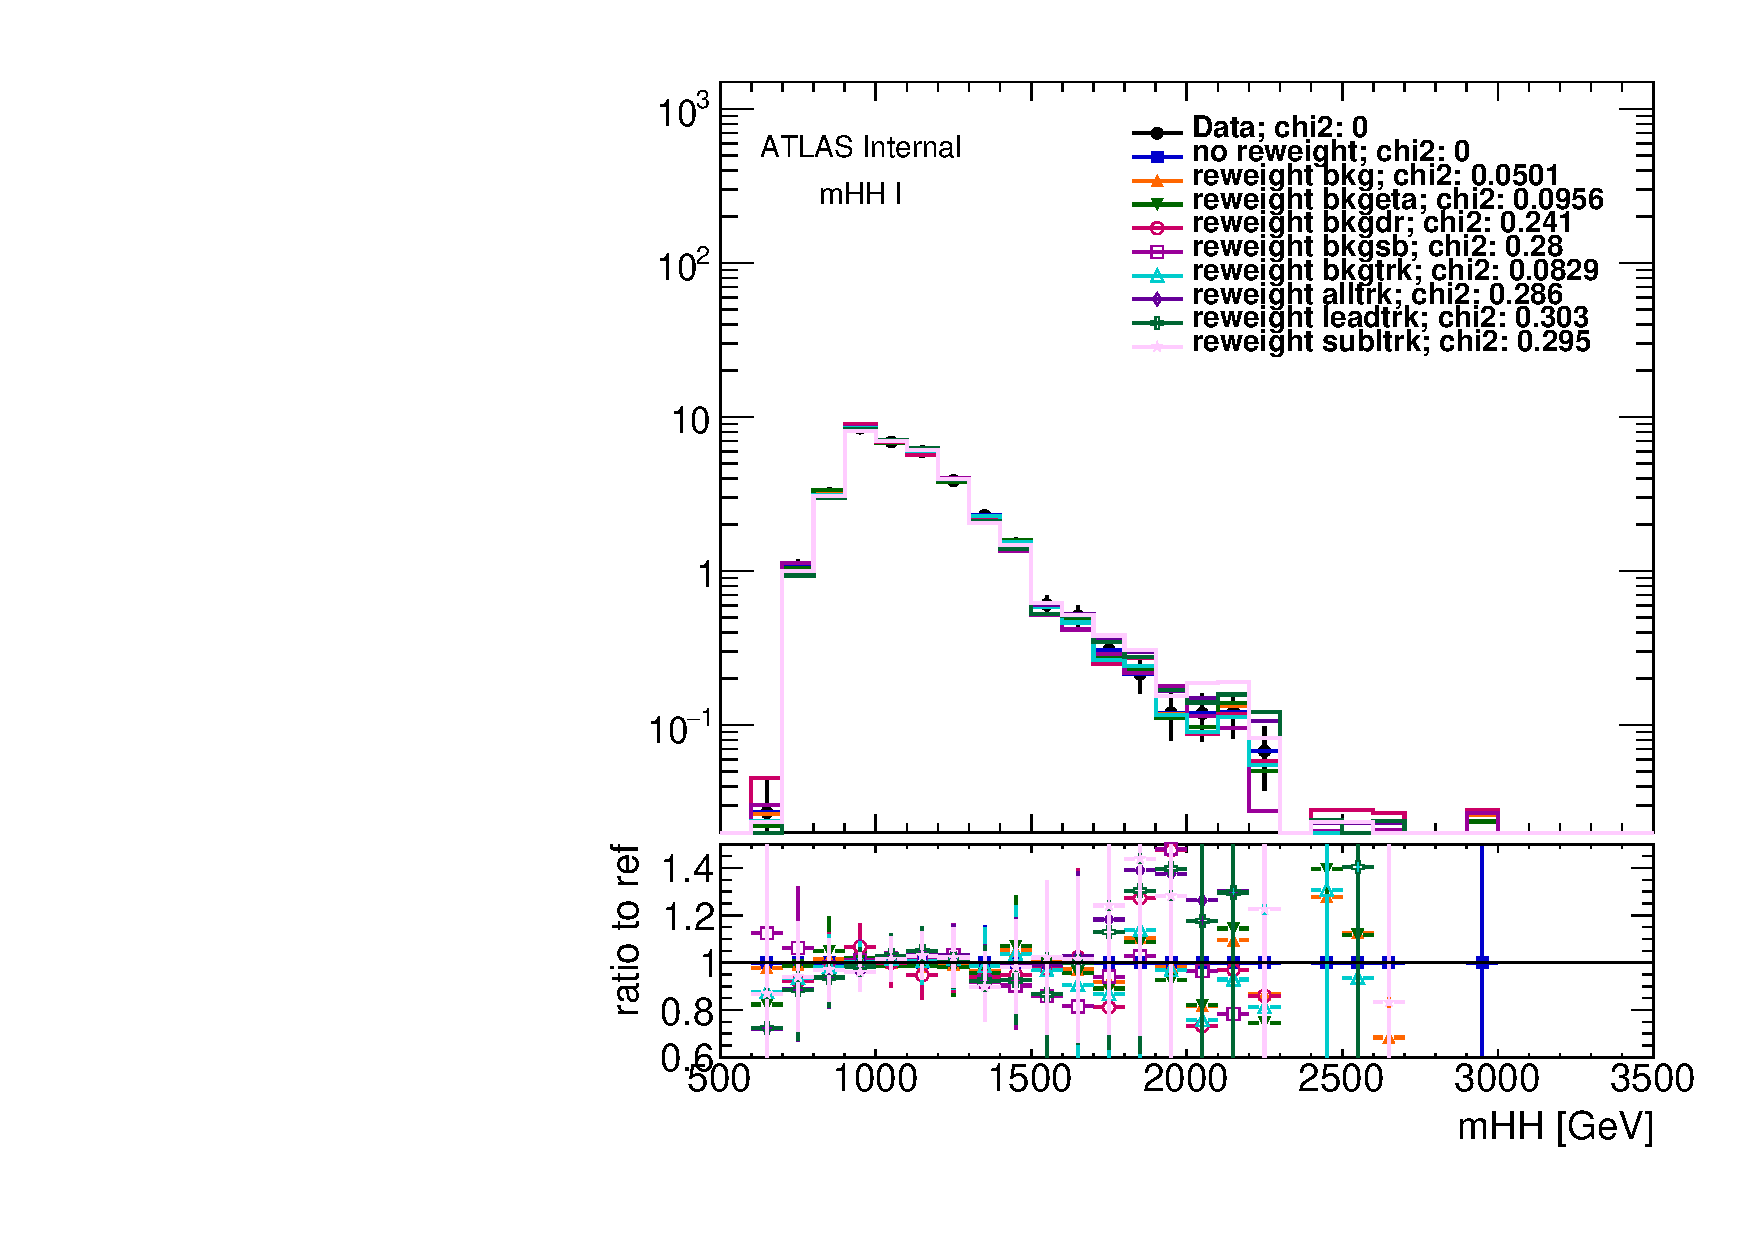
\includegraphics[width=0.4\textwidth,angle=-90]{figures/boosted/AppendixReweight/Compare/Data_FourTag_Signal_directcompare_mHH_l_1.pdf}
\caption{Reweighted $4b$ Sideband (top)/Control (middle)/Signal(bottom) region predictions comaprison, for MJJ. The Signal region is blinded, where the distribution is replaced with the non-reweighted distributions.}
\label{fig:app-rw-comp-4b}
\end{center}
\end{figure*}


\begin{figure*}[htbp!]
\begin{center}
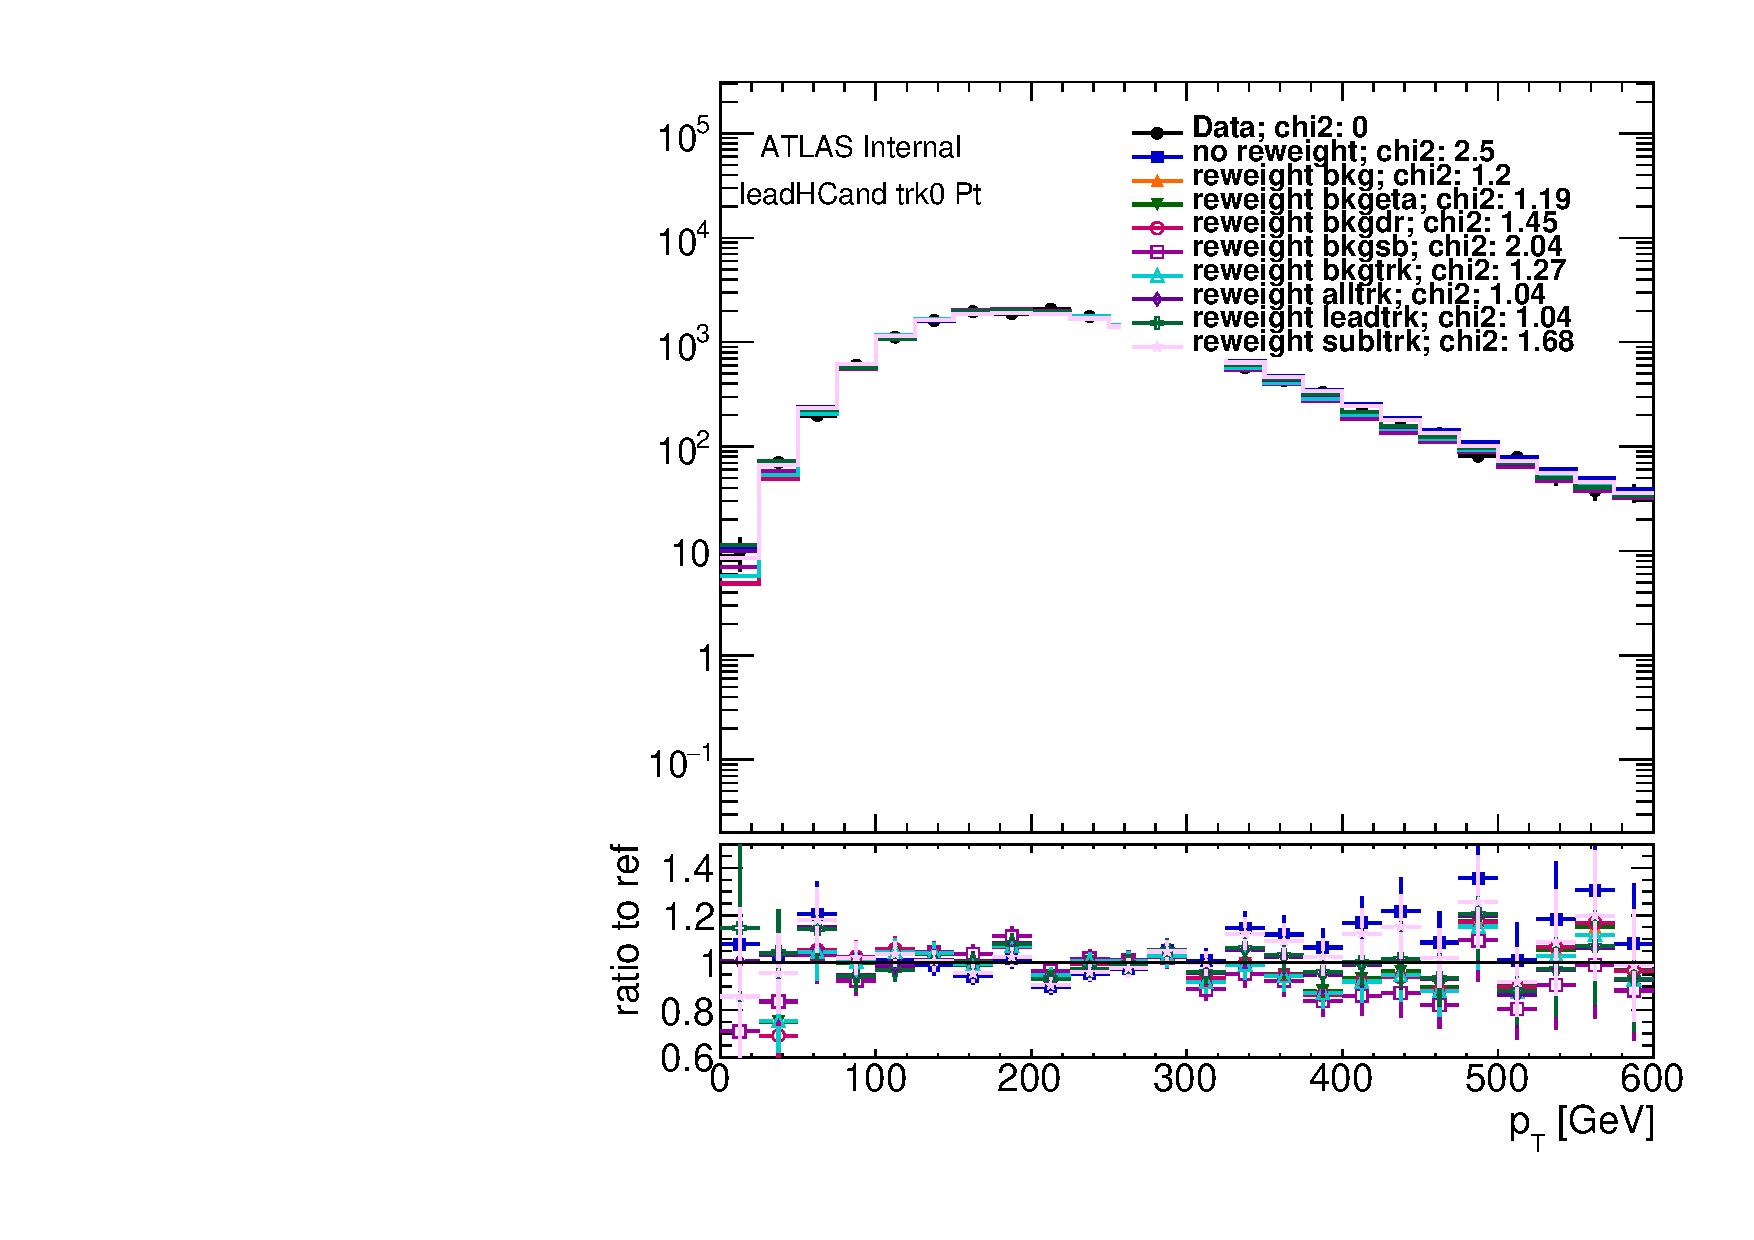
\includegraphics[width=0.24\textwidth,angle=-90]{figures/boosted/AppendixReweight/Compare/Data_TwoTag_split_Sideband_directcompare_leadHCand_trk0_Pt_1.pdf}
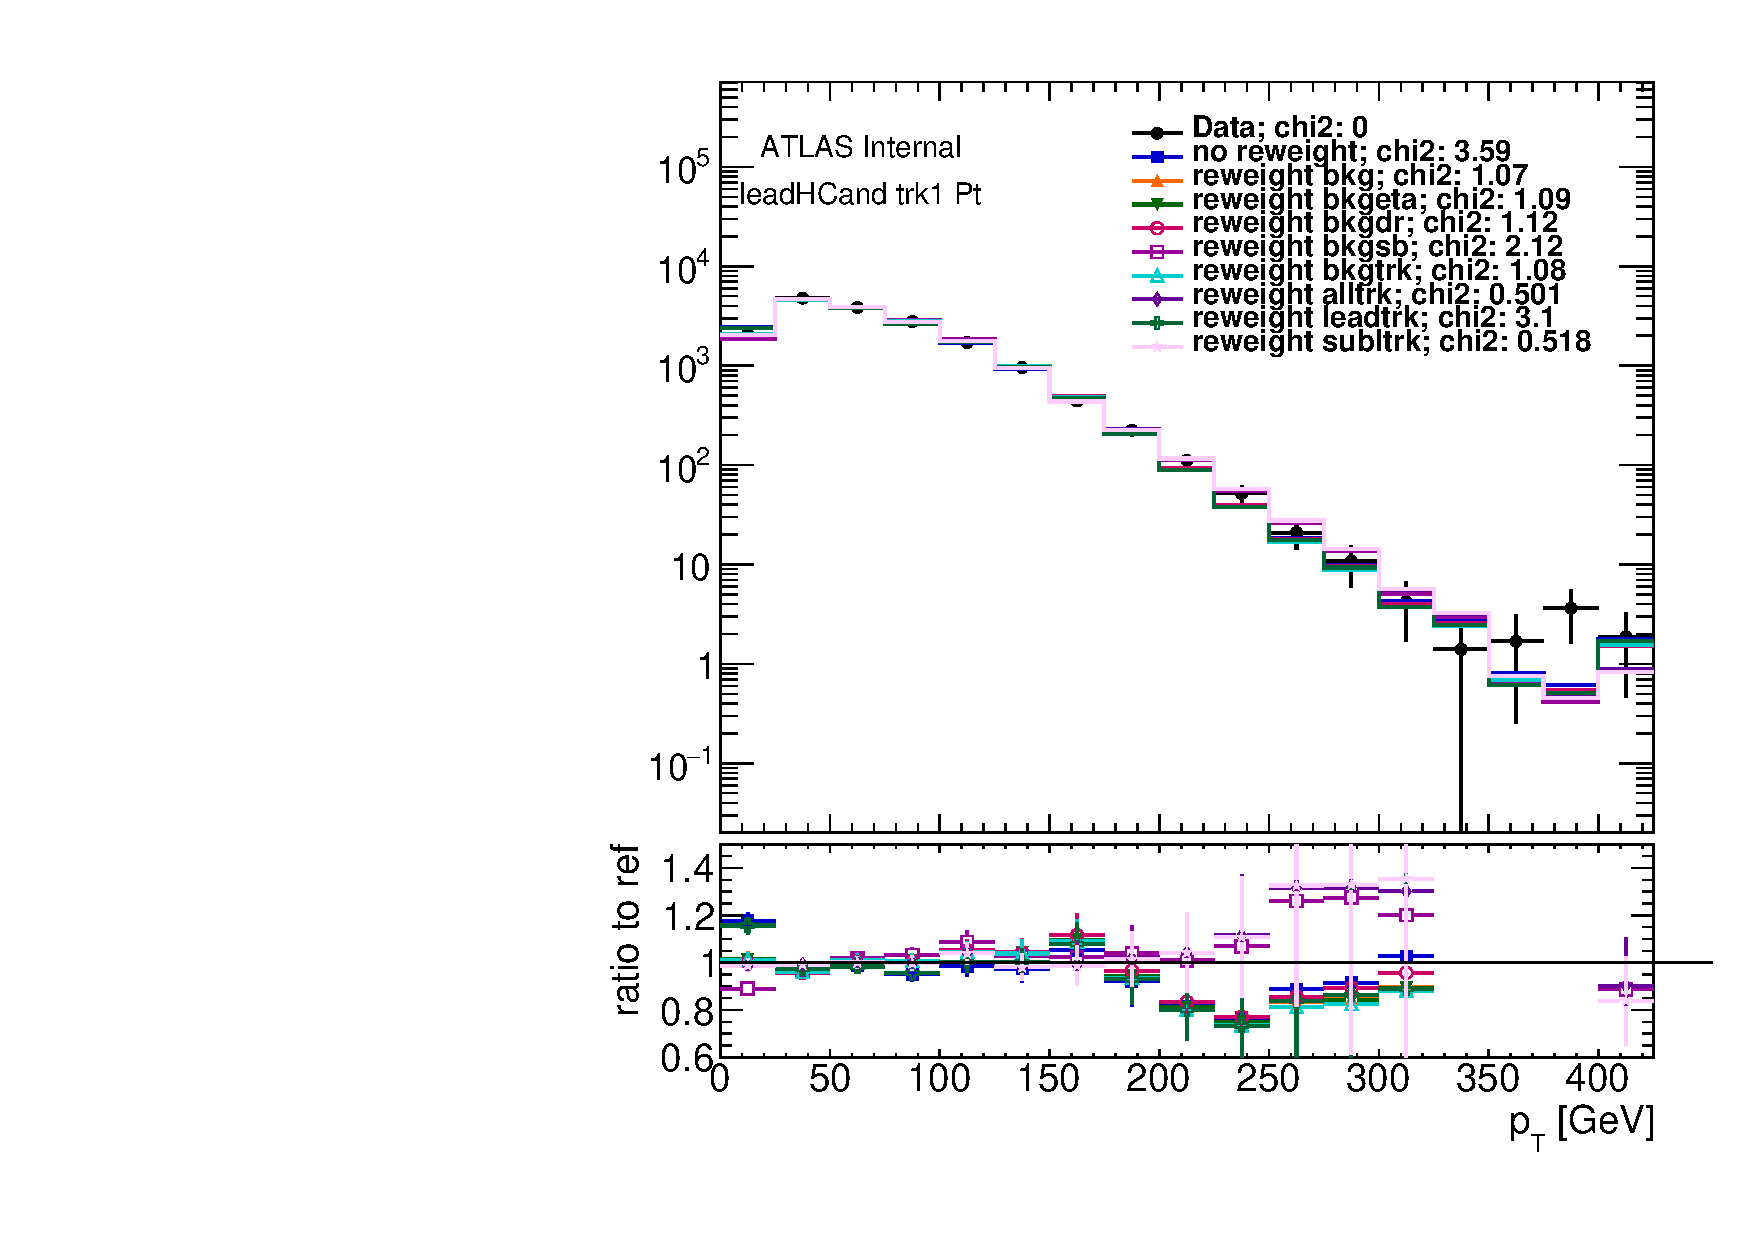
\includegraphics[width=0.24\textwidth,angle=-90]{figures/boosted/AppendixReweight/Compare/Data_TwoTag_split_Sideband_directcompare_leadHCand_trk1_Pt_1.pdf}
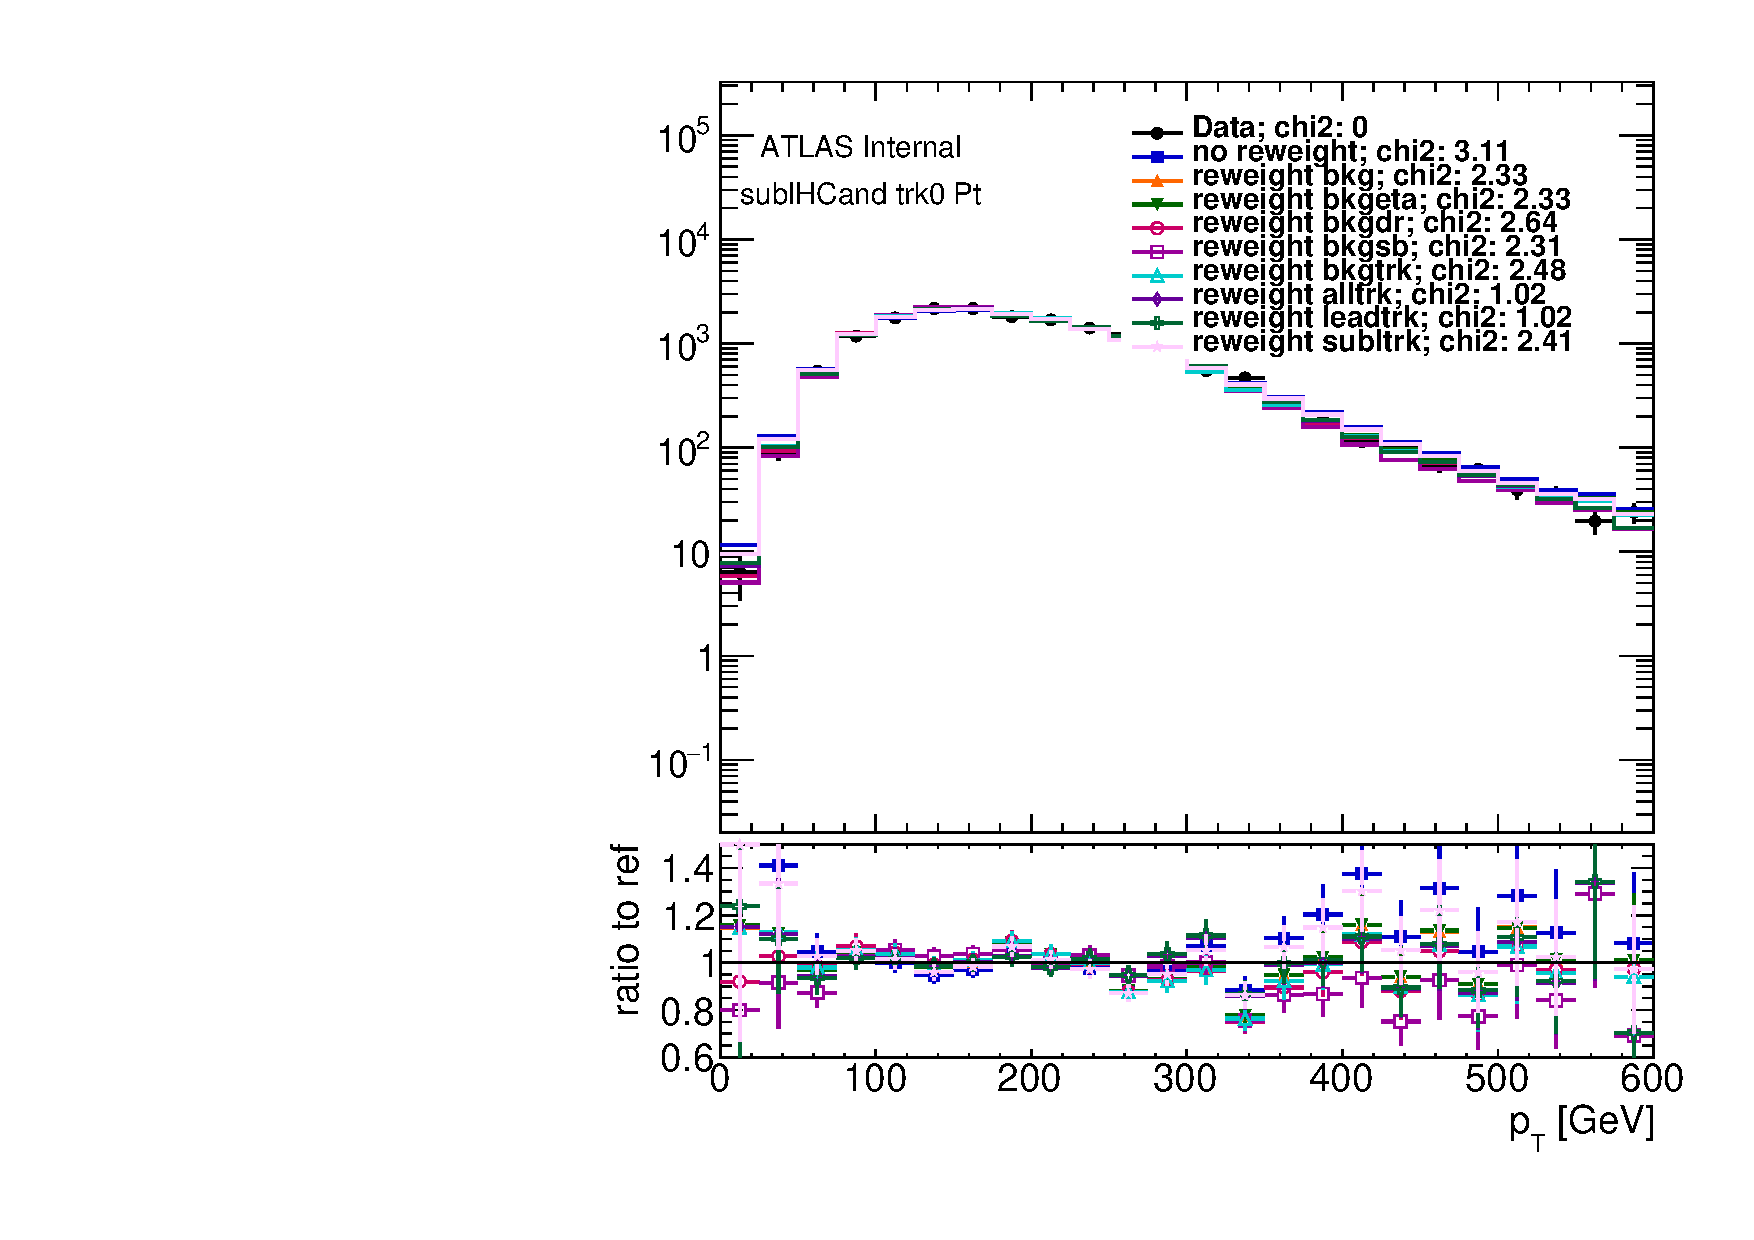
\includegraphics[width=0.24\textwidth,angle=-90]{figures/boosted/AppendixReweight/Compare/Data_TwoTag_split_Sideband_directcompare_sublHCand_trk0_Pt_1.pdf}
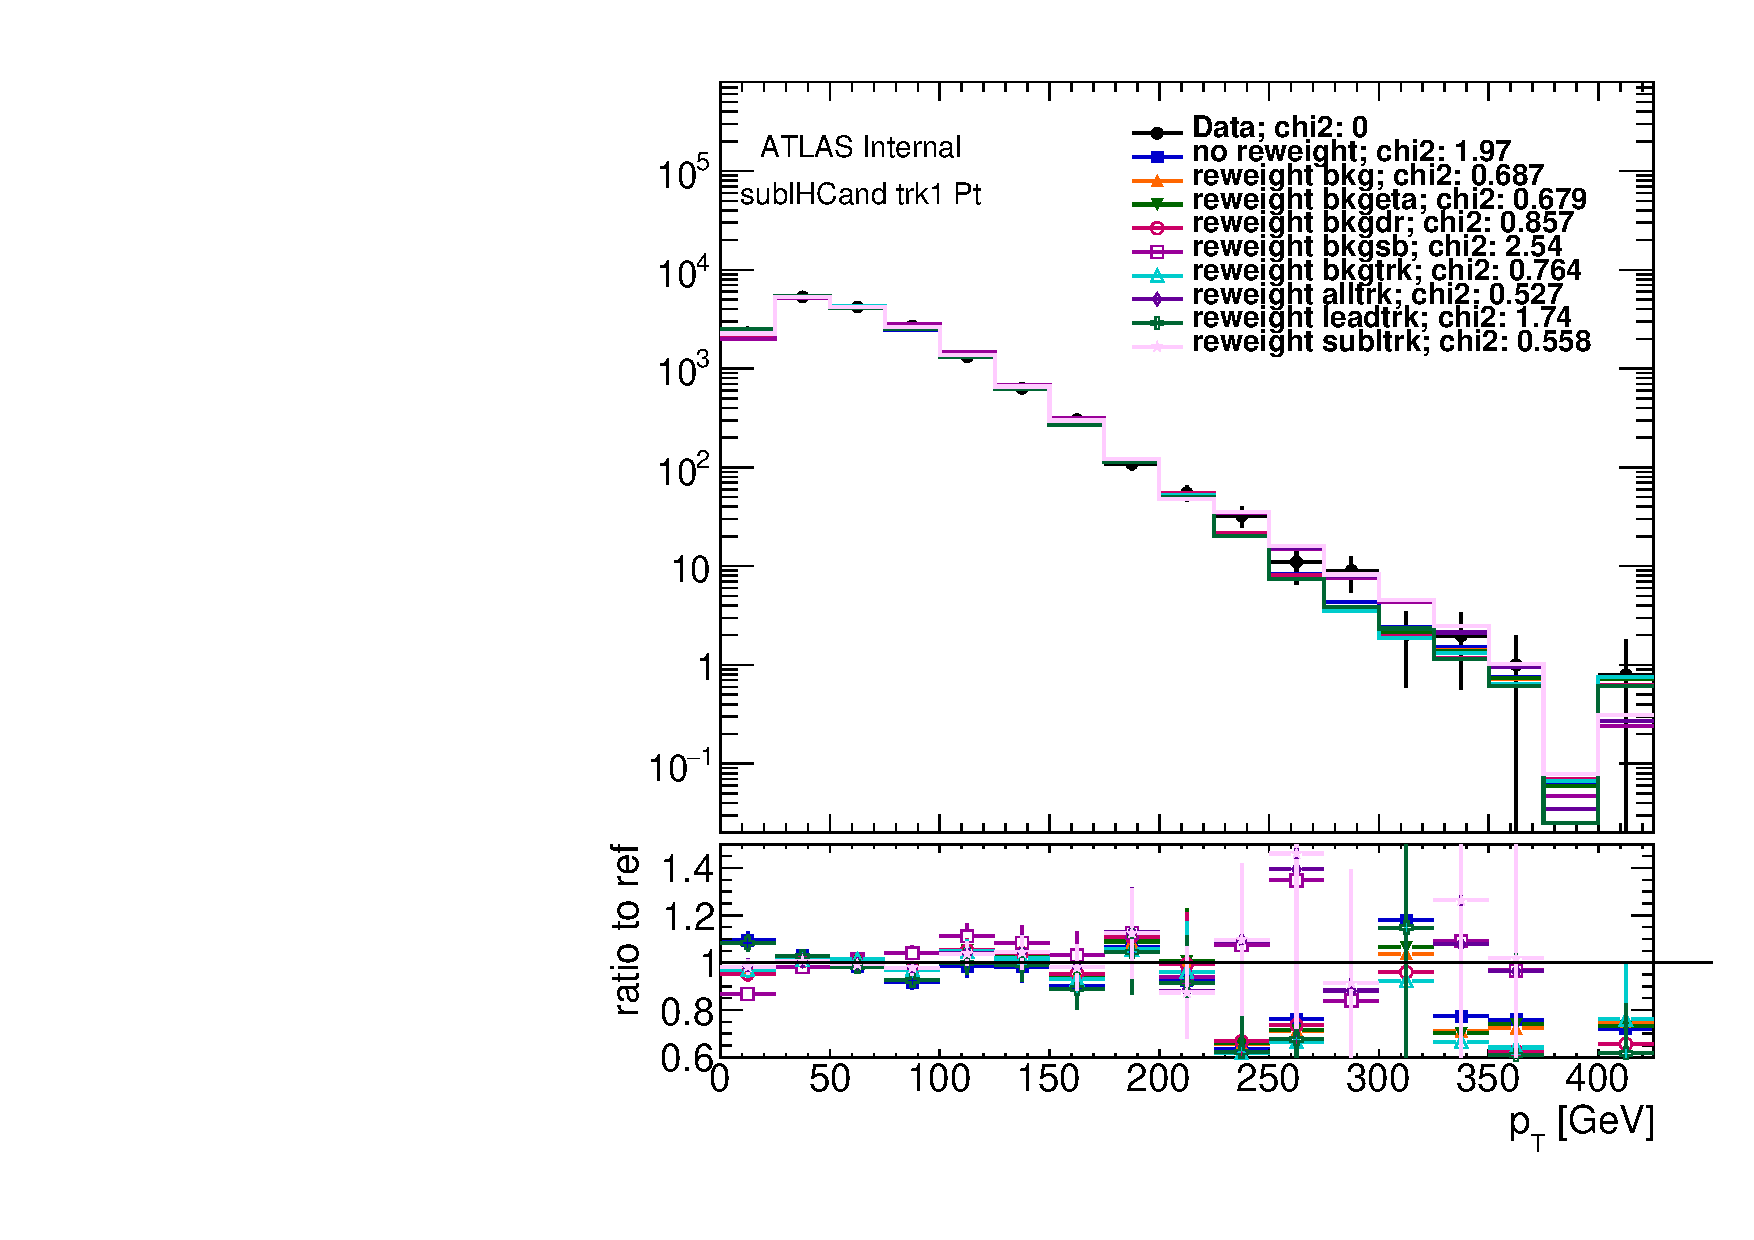
\includegraphics[width=0.24\textwidth,angle=-90]{figures/boosted/AppendixReweight/Compare/Data_TwoTag_split_Sideband_directcompare_sublHCand_trk1_Pt_1.pdf}\\
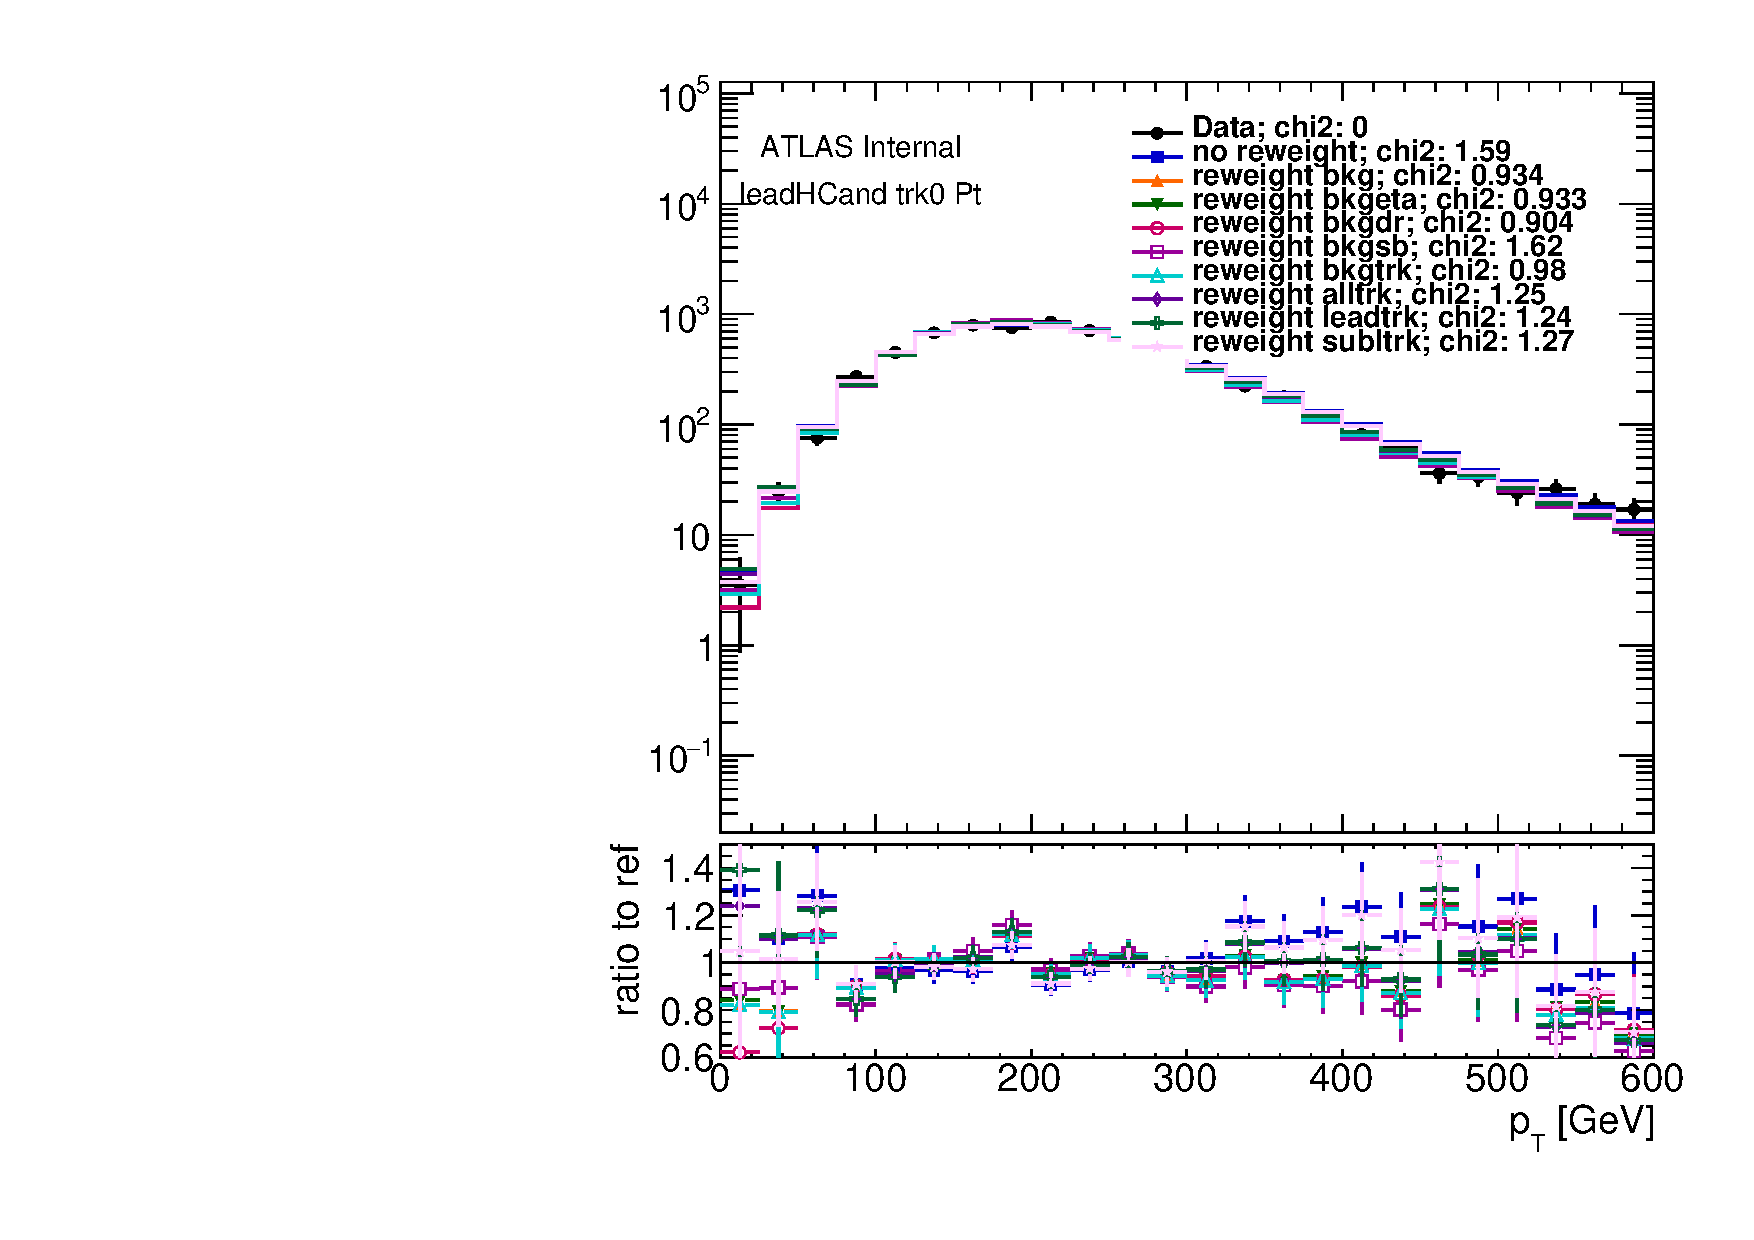
\includegraphics[width=0.24\textwidth,angle=-90]{figures/boosted/AppendixReweight/Compare/Data_TwoTag_split_Control_directcompare_leadHCand_trk0_Pt_1.pdf}
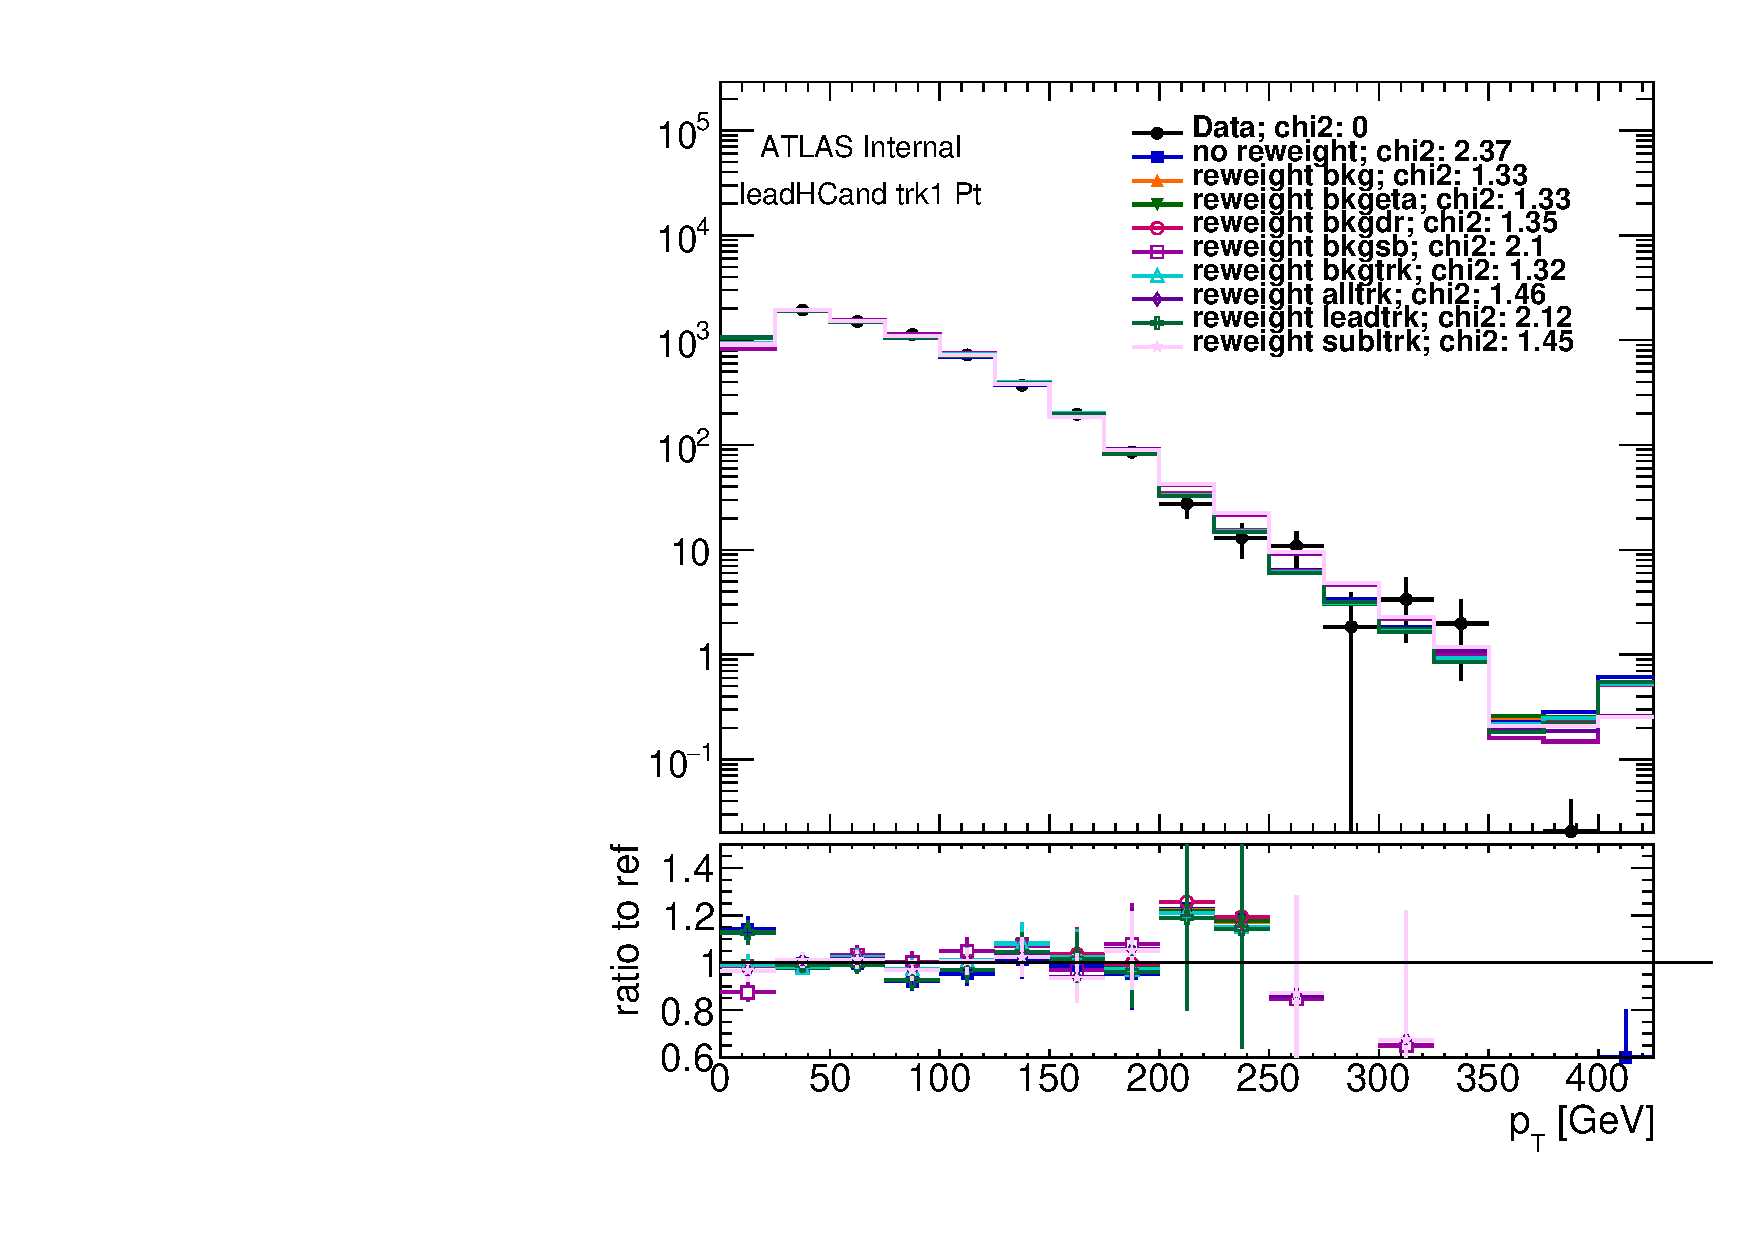
\includegraphics[width=0.24\textwidth,angle=-90]{figures/boosted/AppendixReweight/Compare/Data_TwoTag_split_Control_directcompare_leadHCand_trk1_Pt_1.pdf}
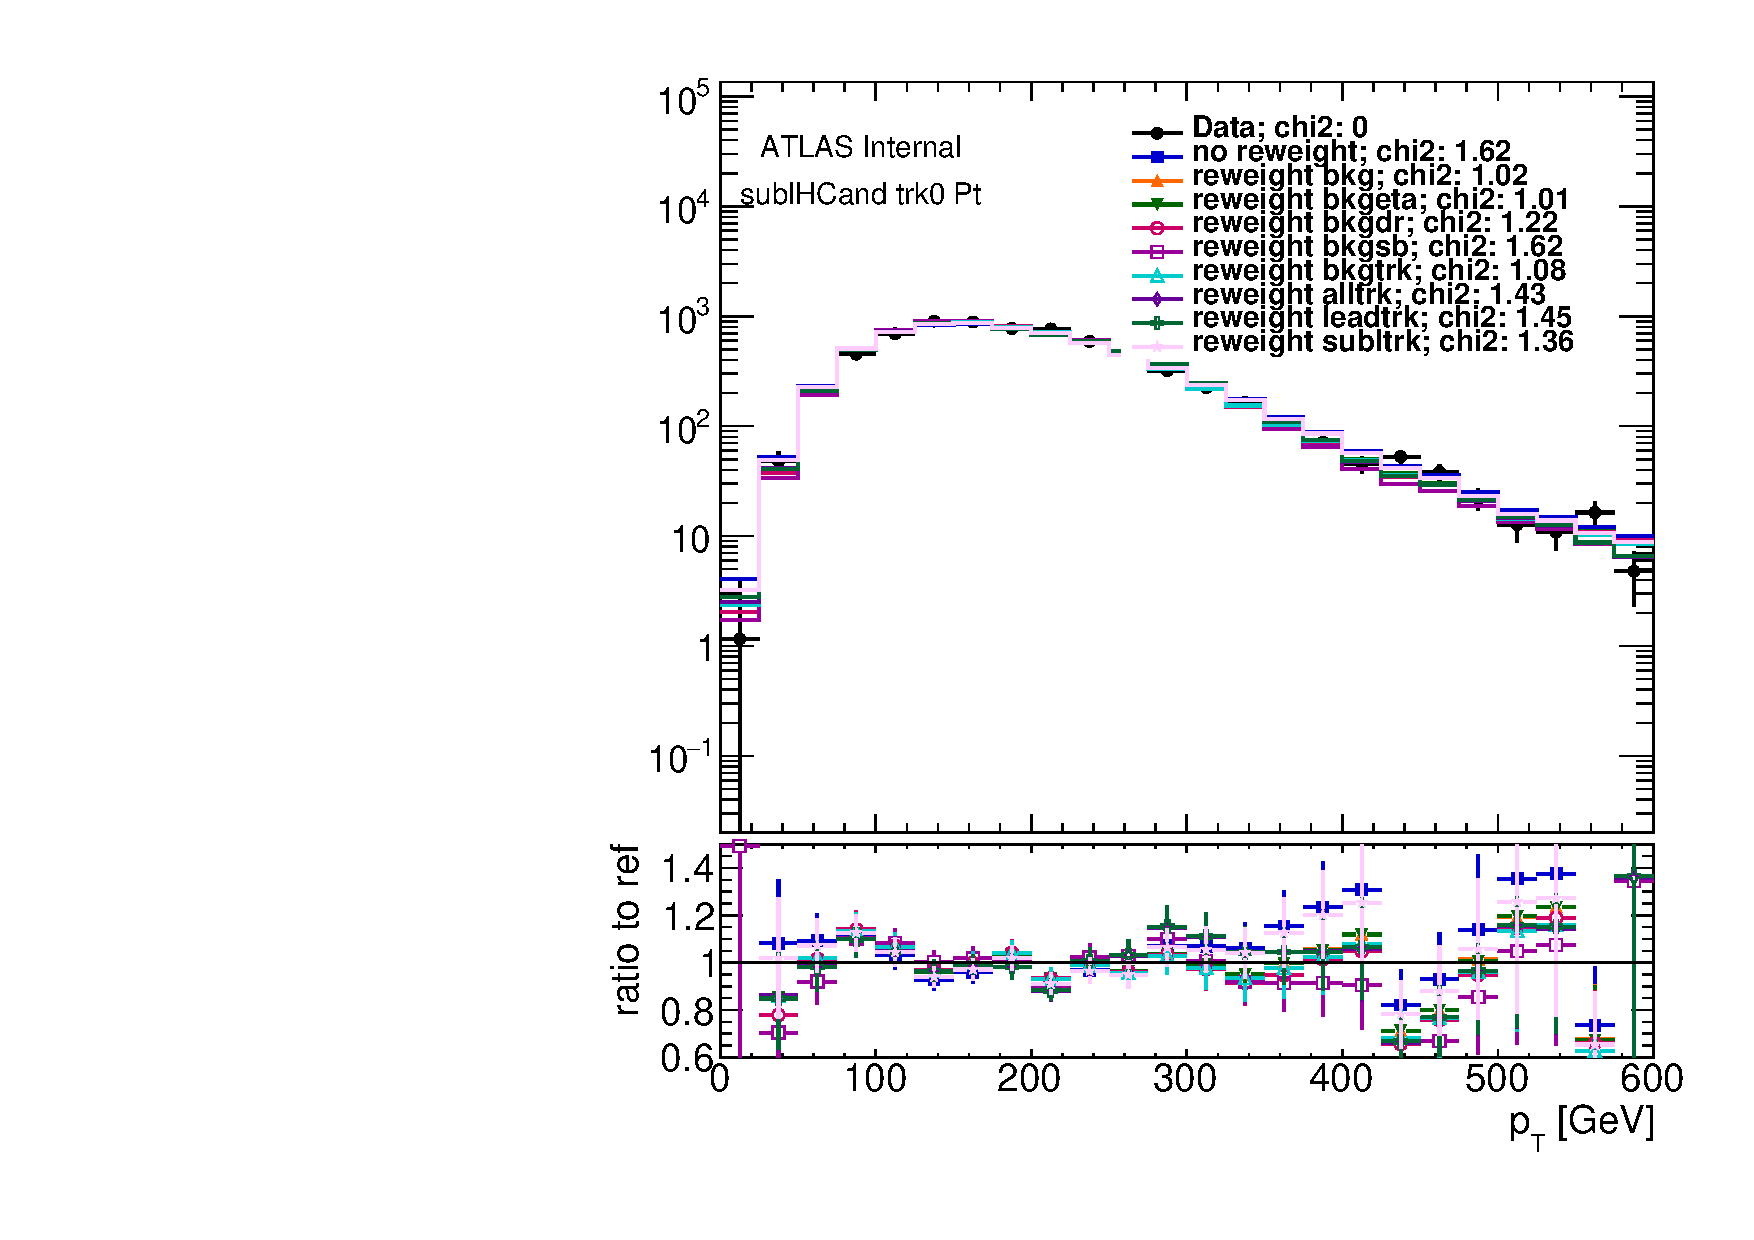
\includegraphics[width=0.24\textwidth,angle=-90]{figures/boosted/AppendixReweight/Compare/Data_TwoTag_split_Control_directcompare_sublHCand_trk0_Pt_1.pdf}
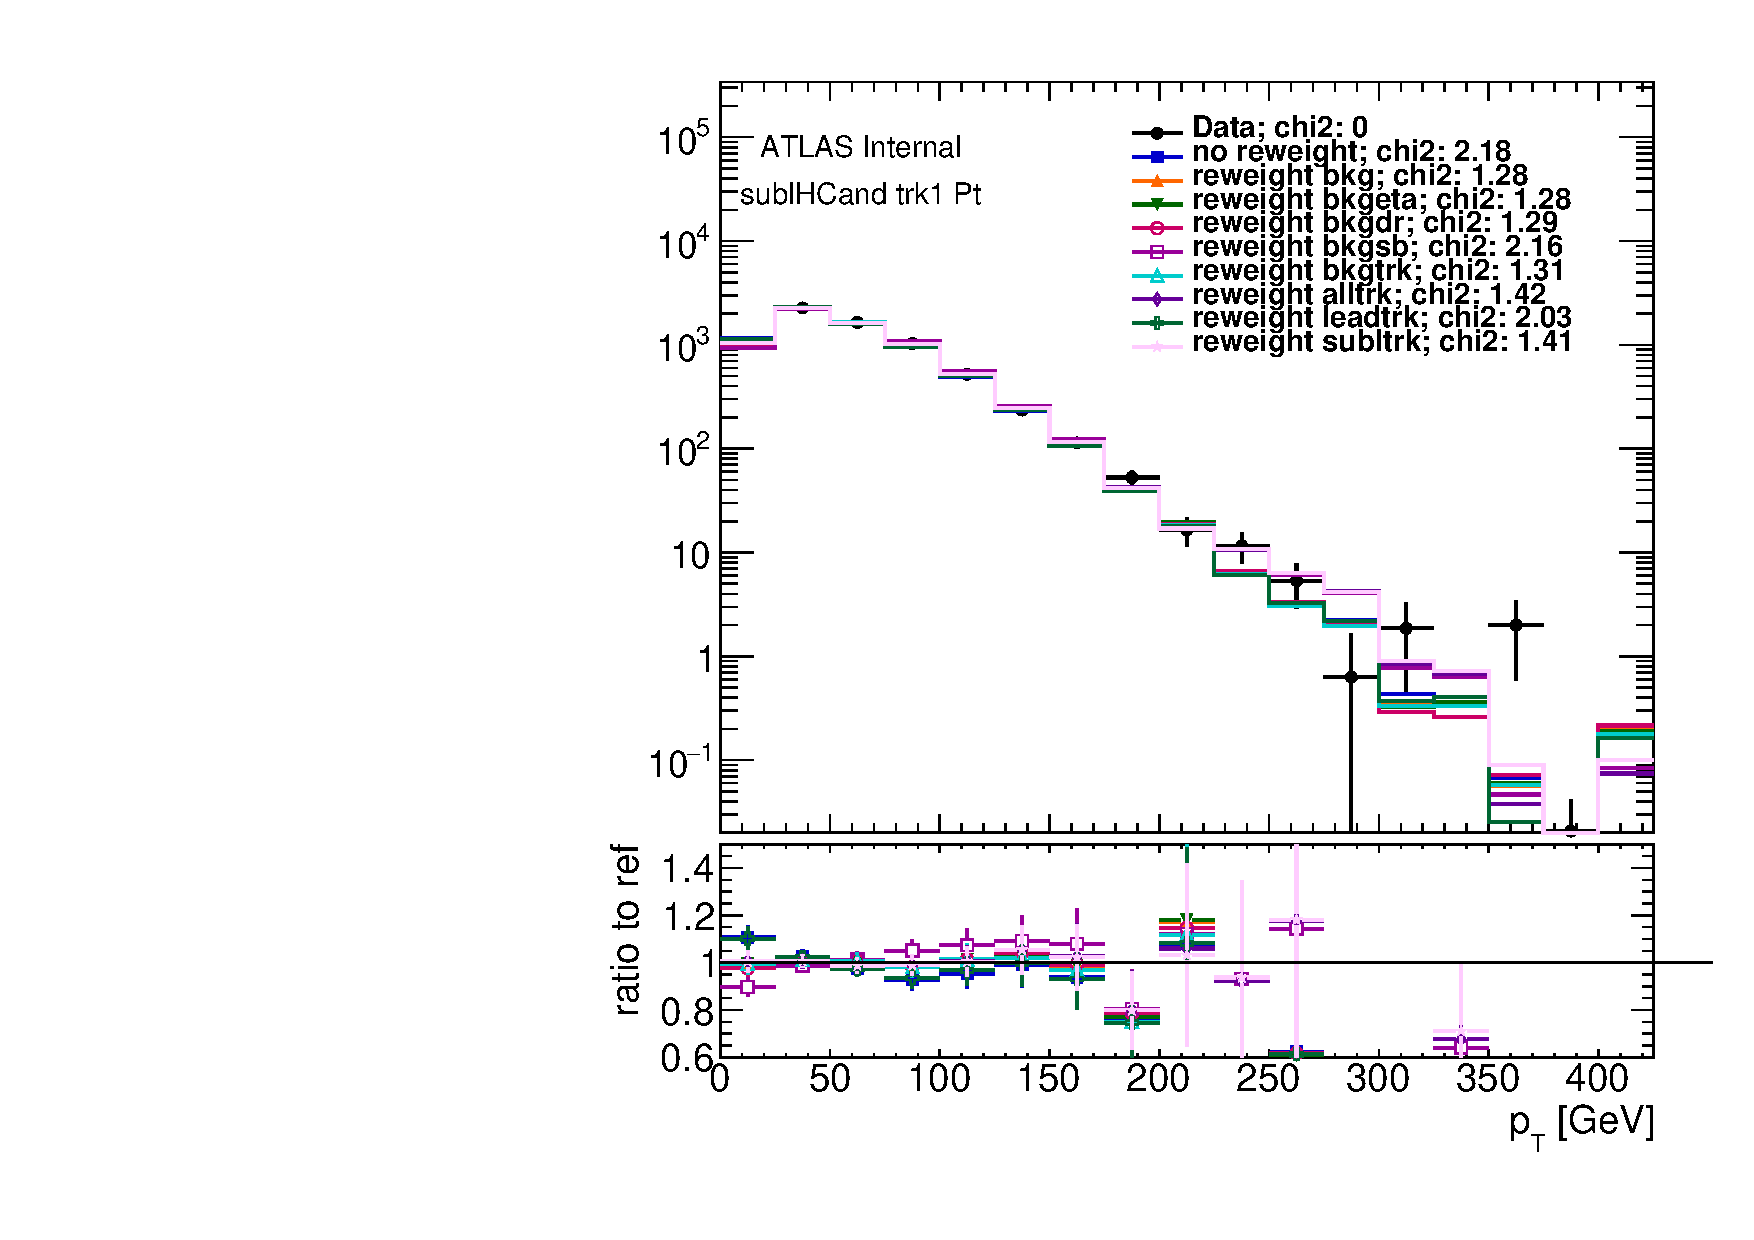
\includegraphics[width=0.24\textwidth,angle=-90]{figures/boosted/AppendixReweight/Compare/Data_TwoTag_split_Control_directcompare_sublHCand_trk1_Pt_1.pdf}\\
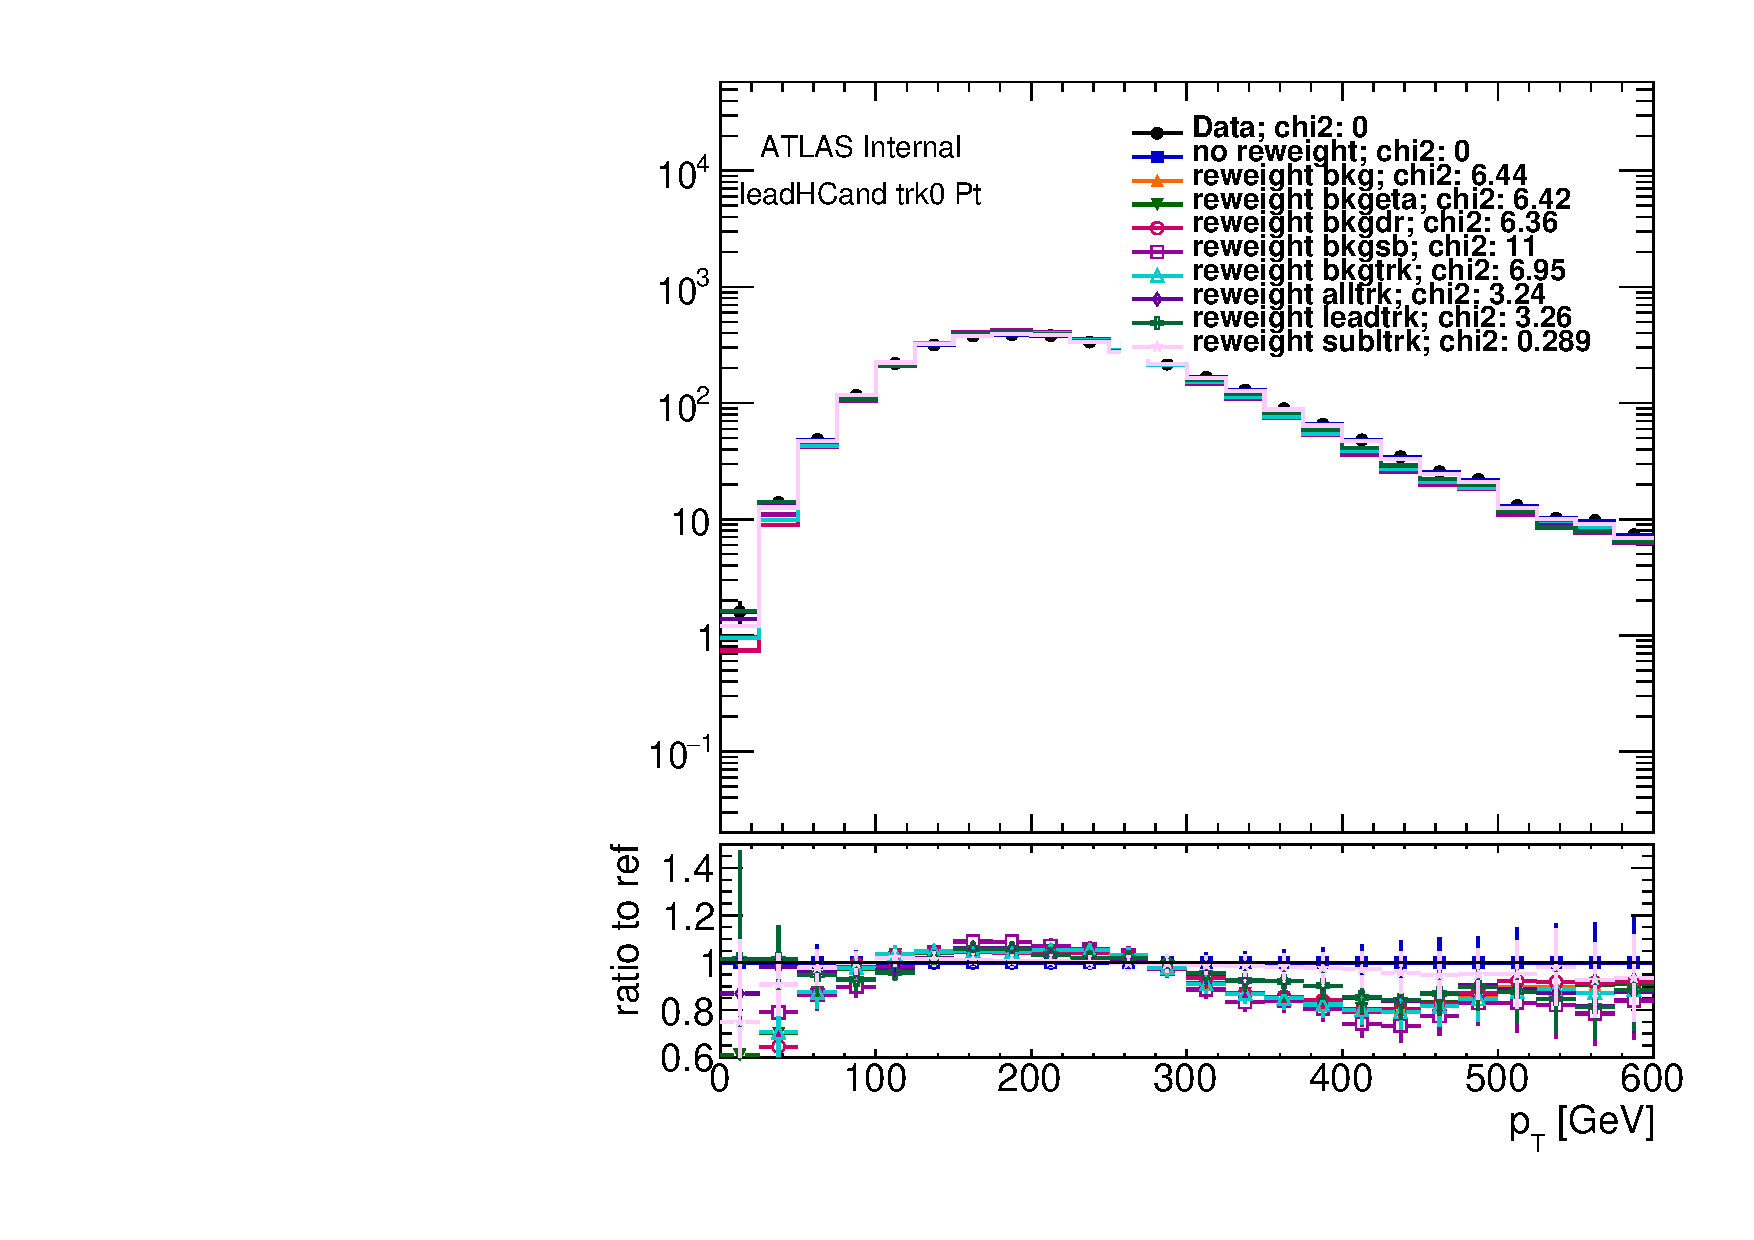
\includegraphics[width=0.24\textwidth,angle=-90]{figures/boosted/AppendixReweight/Compare/Data_TwoTag_split_Signal_directcompare_leadHCand_trk0_Pt_1.pdf}
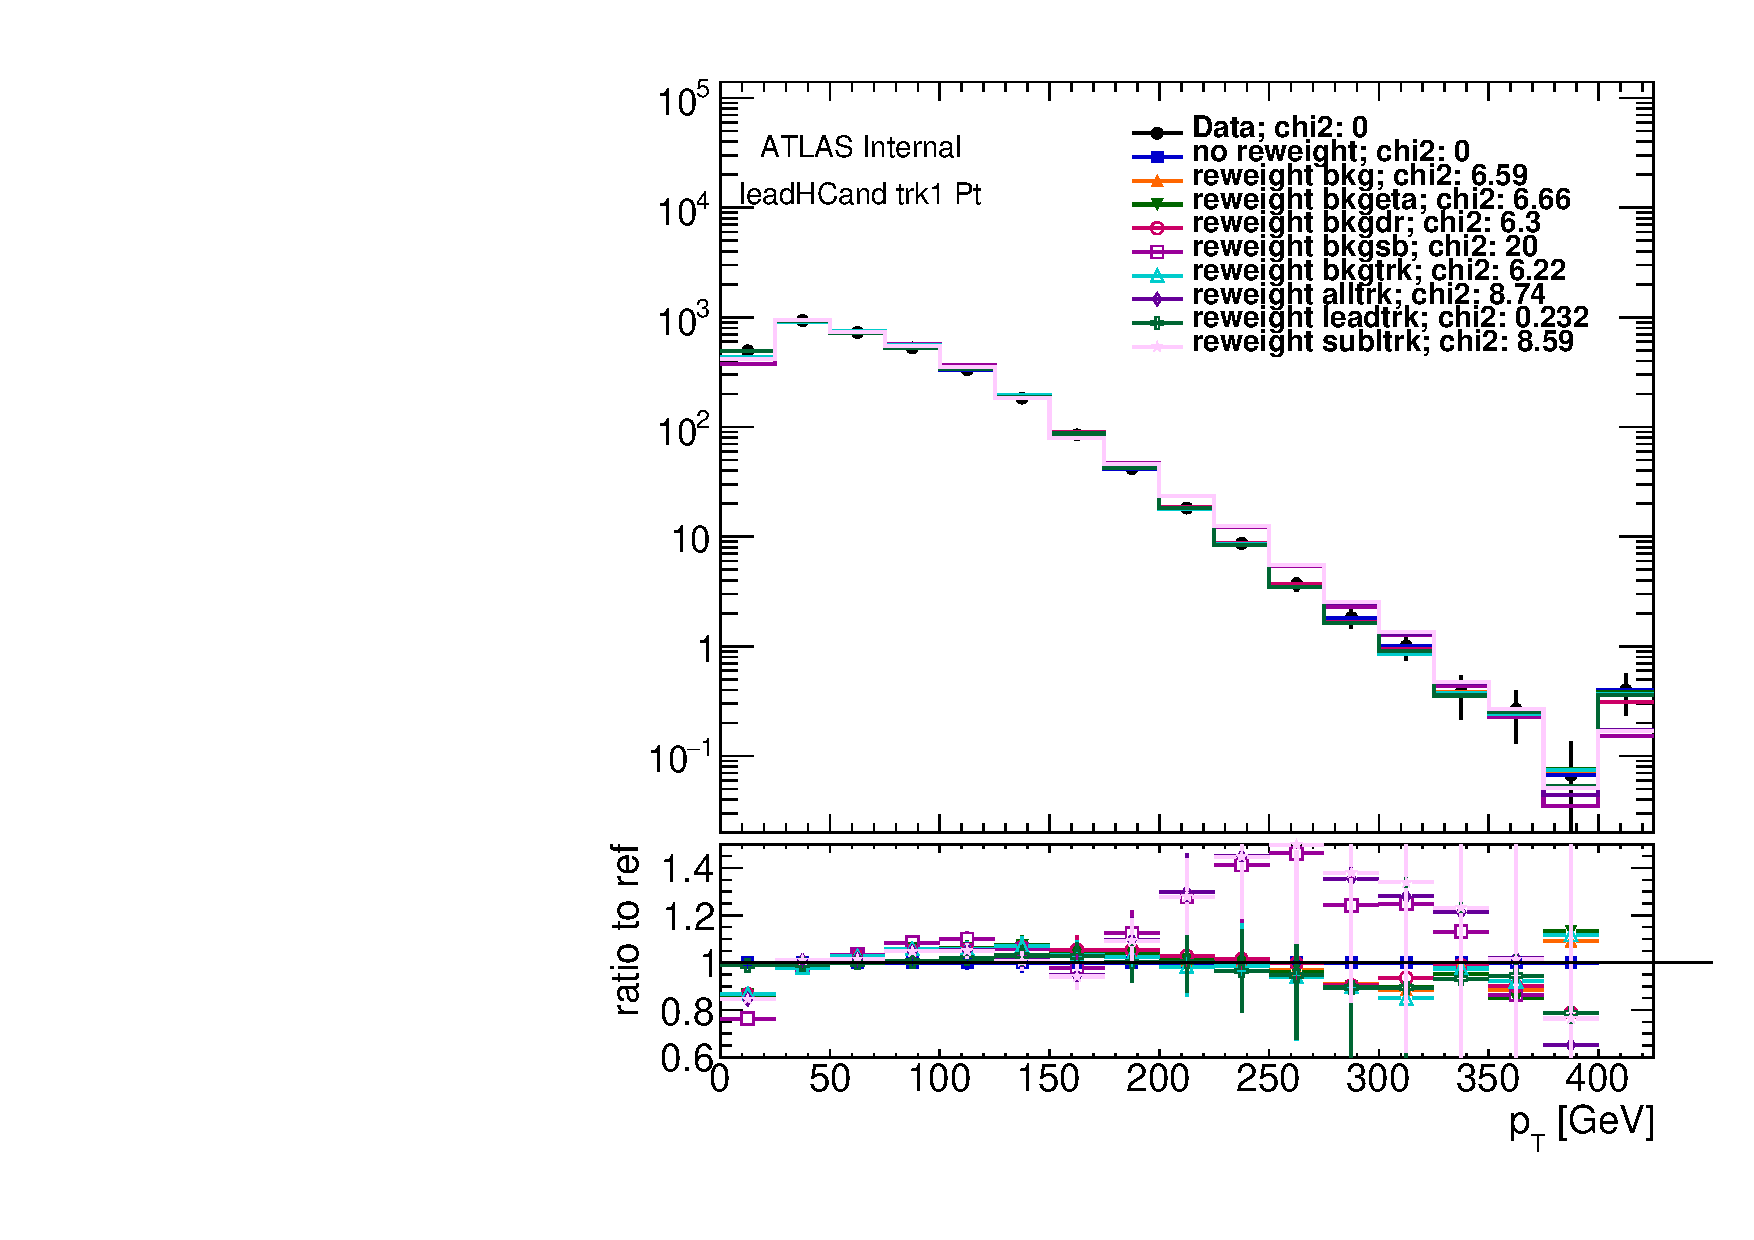
\includegraphics[width=0.24\textwidth,angle=-90]{figures/boosted/AppendixReweight/Compare/Data_TwoTag_split_Signal_directcompare_leadHCand_trk1_Pt_1.pdf}
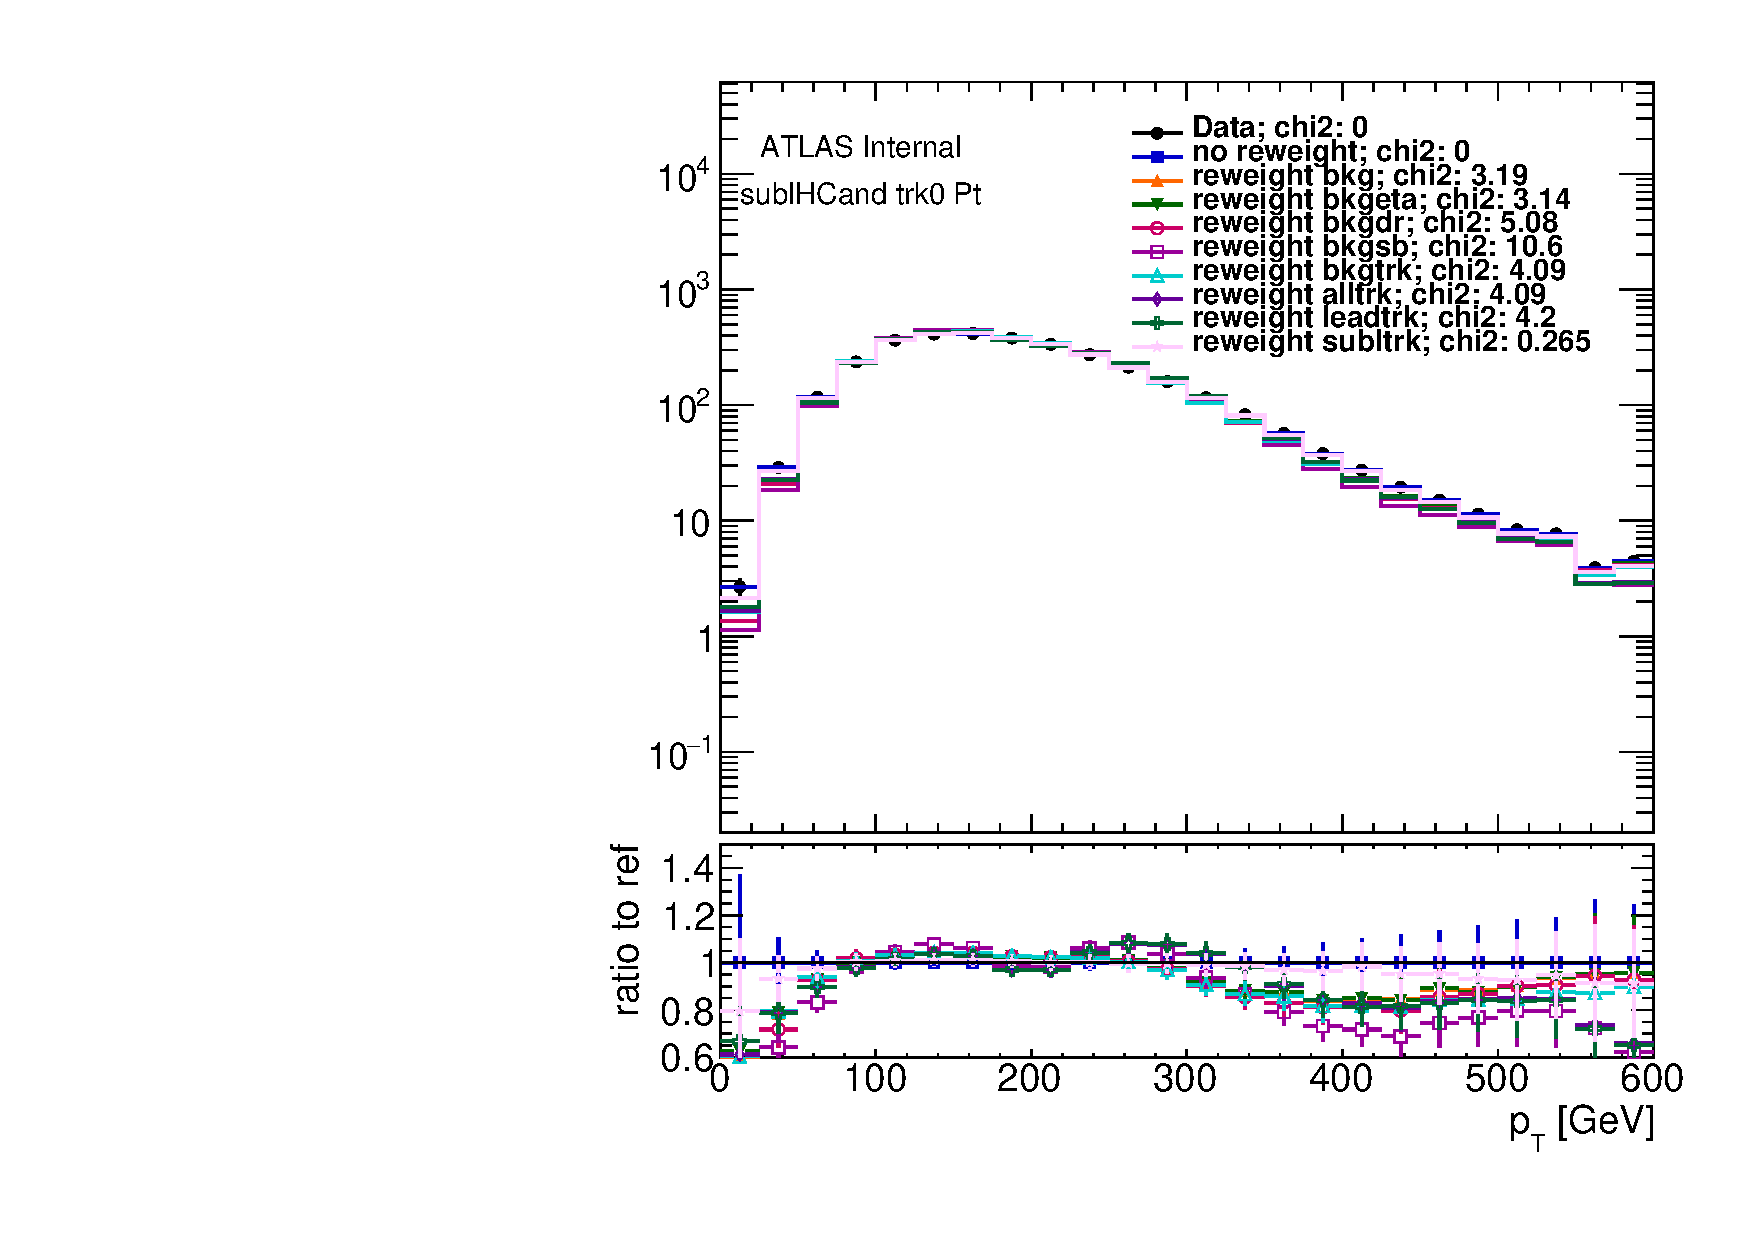
\includegraphics[width=0.24\textwidth,angle=-90]{figures/boosted/AppendixReweight/Compare/Data_TwoTag_split_Signal_directcompare_sublHCand_trk0_Pt_1.pdf}
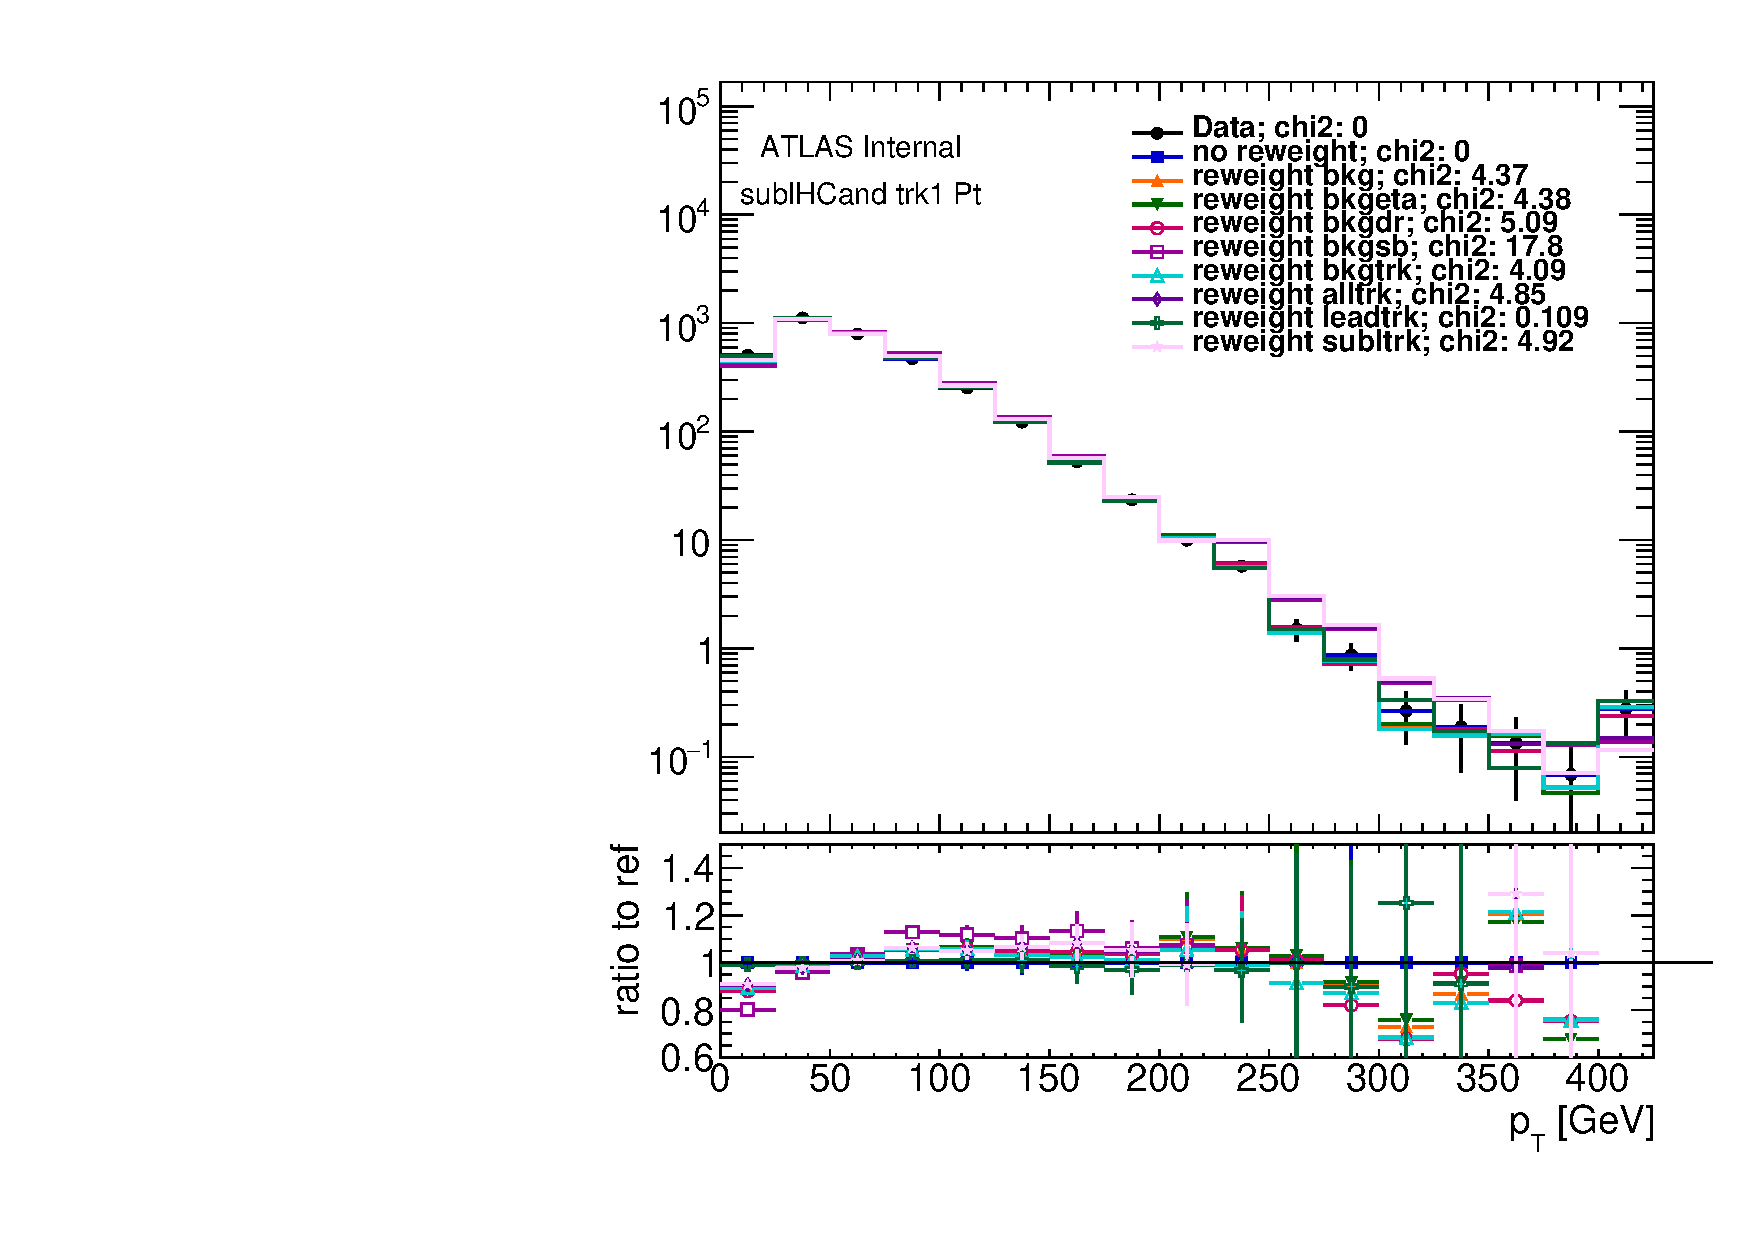
\includegraphics[width=0.24\textwidth,angle=-90]{figures/boosted/AppendixReweight/Compare/Data_TwoTag_split_Signal_directcompare_sublHCand_trk1_Pt_1.pdf}\\
\caption{Reweighted $2bs$ Sideband (top)/Control (middle)/Signal(bottom) region predictions comaprison, for leading Higgs Candidate leading trackjet \pt (first column),  leading Higgs Candidate subleading trackjet \pt (second column), subleading Higgs Candidate leading trackjet \pt (third column), subleading Higgs Candidate subleading trackjet \pt (fourth column). The Signal region is blinded, where the distribution is replaced with the non-reweighted distributions.}
\label{fig:app-rw-comp-2bs-trkjet}
\end{center}
\end{figure*}

\begin{figure*}[htbp!]
\begin{center}
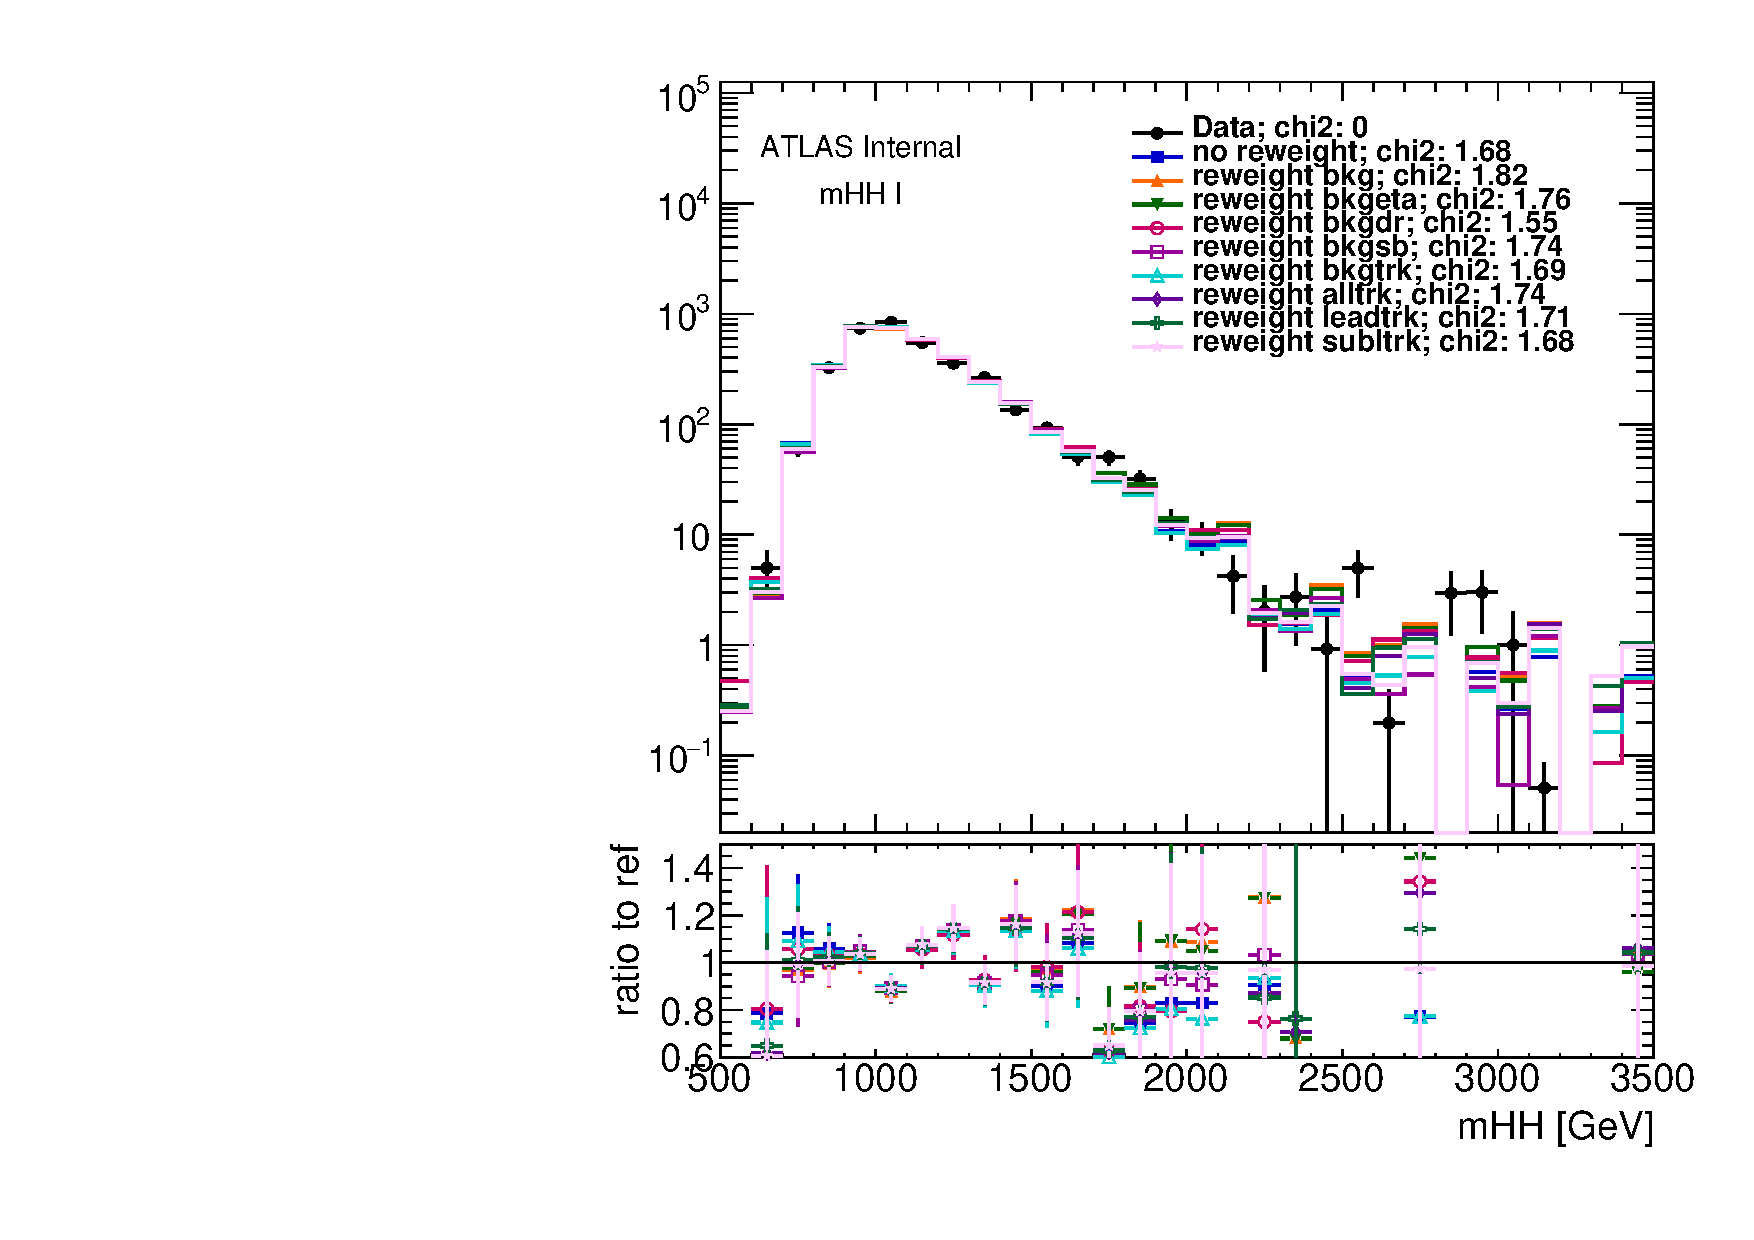
\includegraphics[width=0.4\textwidth,angle=-90]{figures/boosted/AppendixReweight/Compare/Data_ThreeTag_Sideband_directcompare_mHH_l_1.pdf}\\
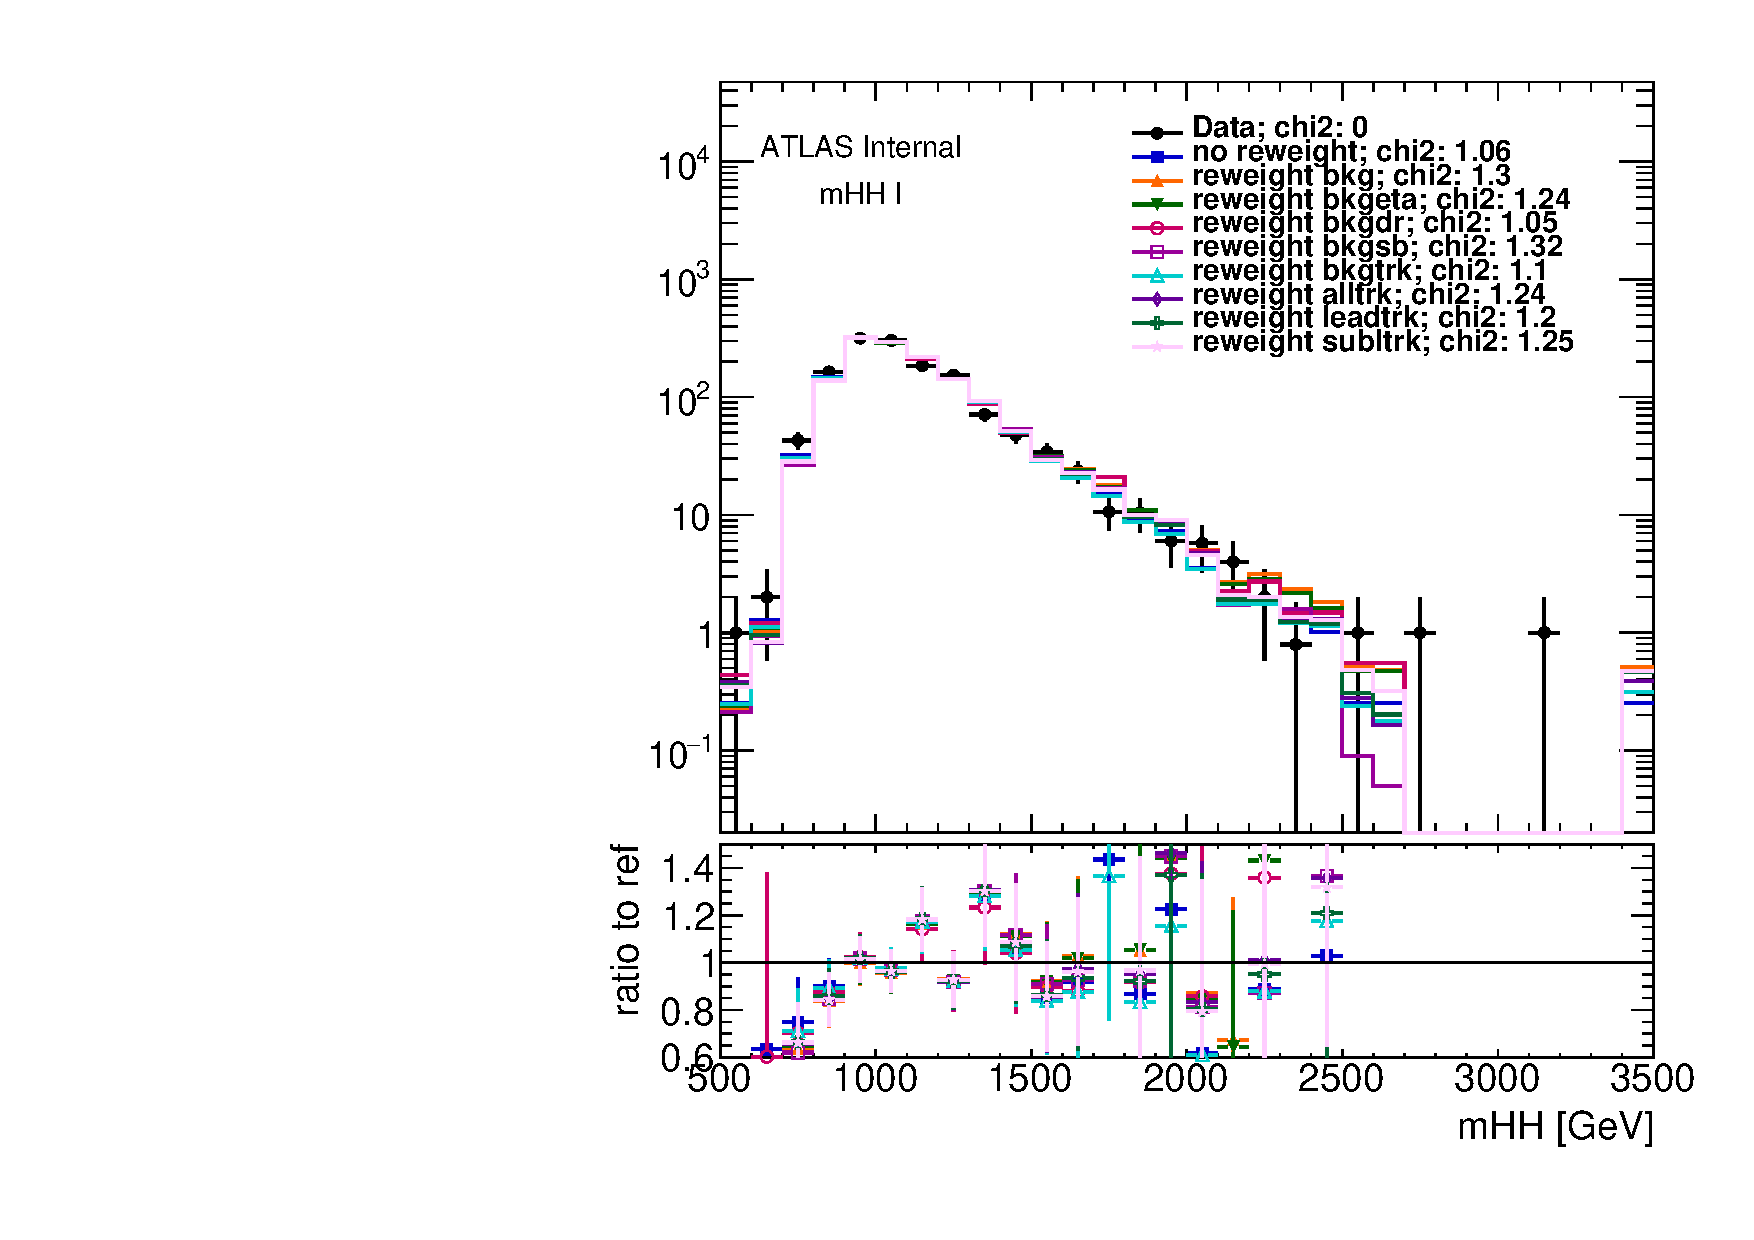
\includegraphics[width=0.4\textwidth,angle=-90]{figures/boosted/AppendixReweight/Compare/Data_ThreeTag_Control_directcompare_mHH_l_1.pdf}\\
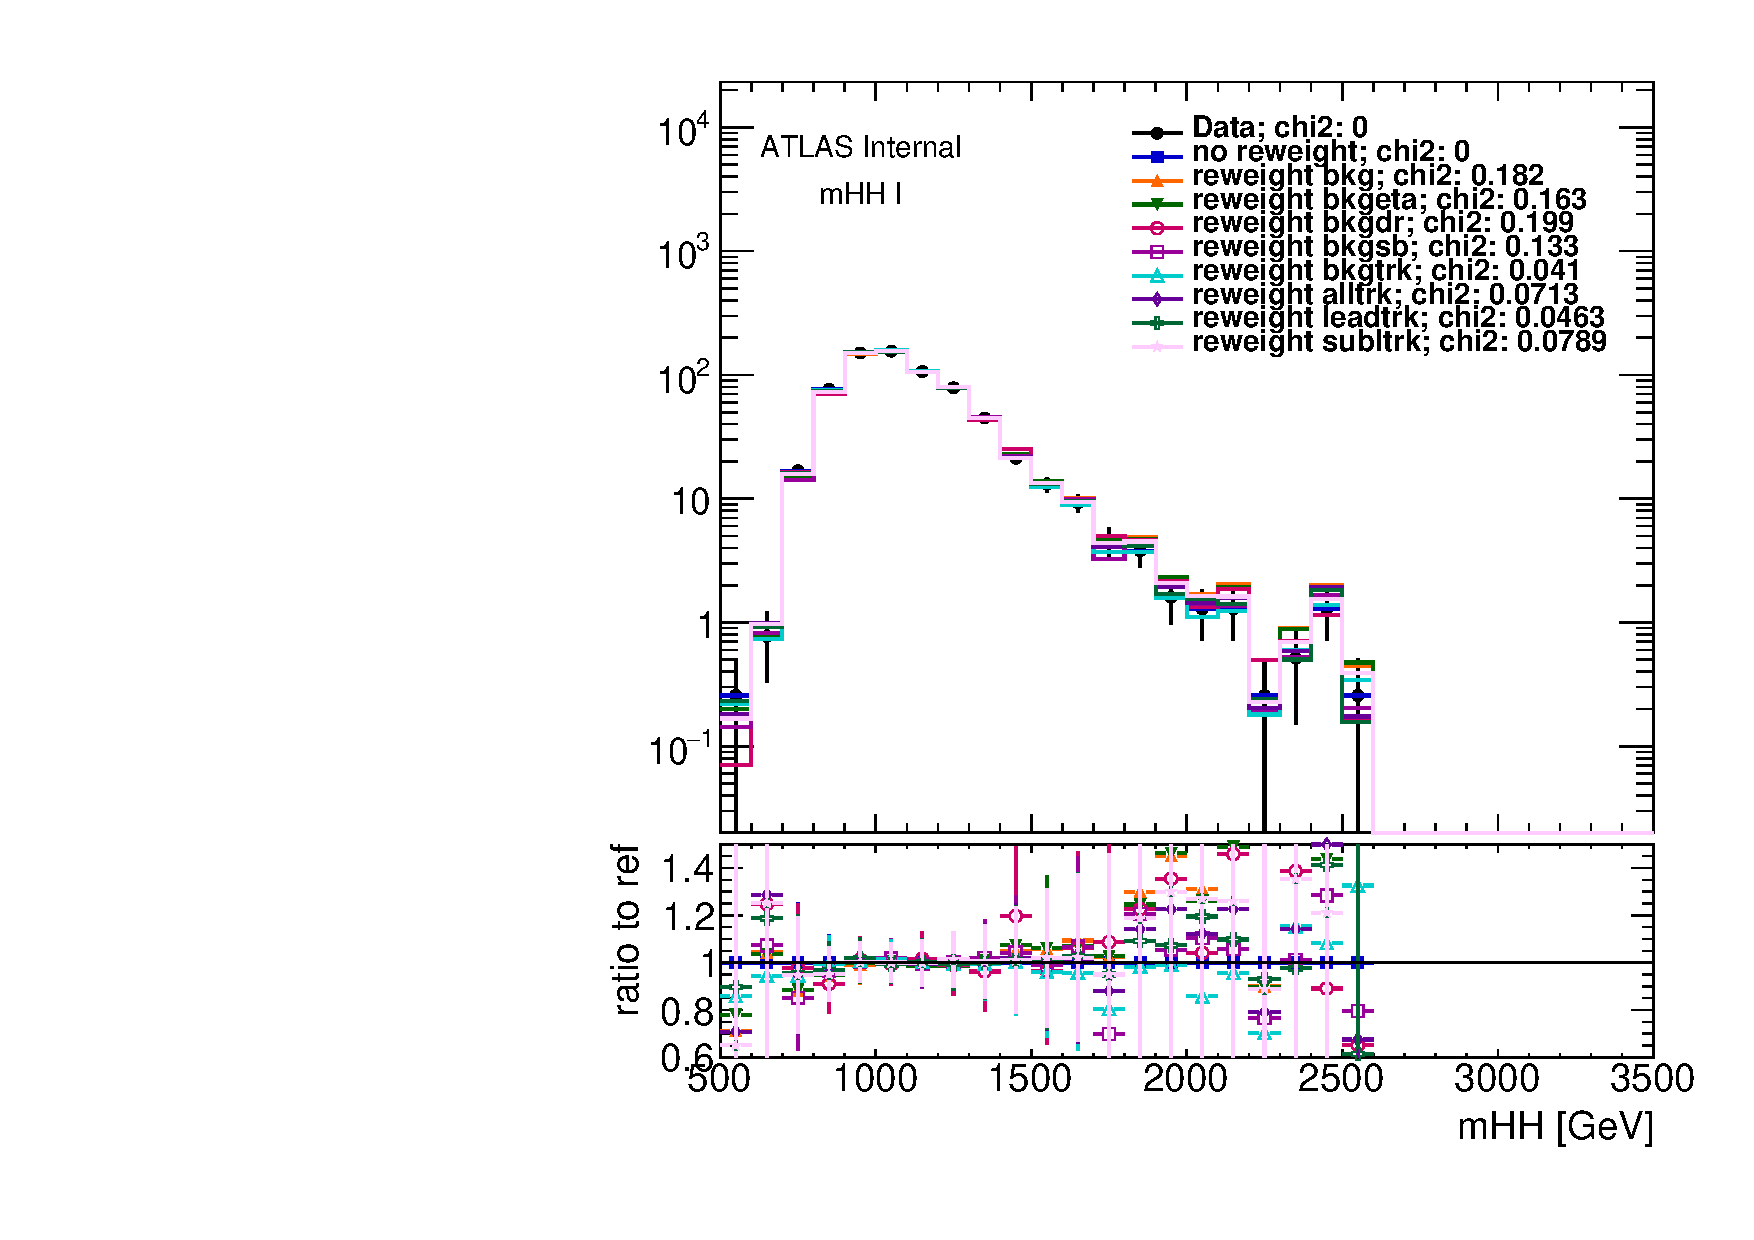
\includegraphics[width=0.4\textwidth,angle=-90]{figures/boosted/AppendixReweight/Compare/Data_ThreeTag_Signal_directcompare_mHH_l_1.pdf}
\caption{Reweighted $3b$ Sideband (top)/Control (middle)/Signal(bottom) region predictions comaprison, for MJJ. The Signal region is blinded, where the distribution is replaced with the non-reweighted distributions.}
\label{fig:app-rw-comp-3b}
\end{center}
\end{figure*}

\begin{figure*}[htbp!]
\begin{center}
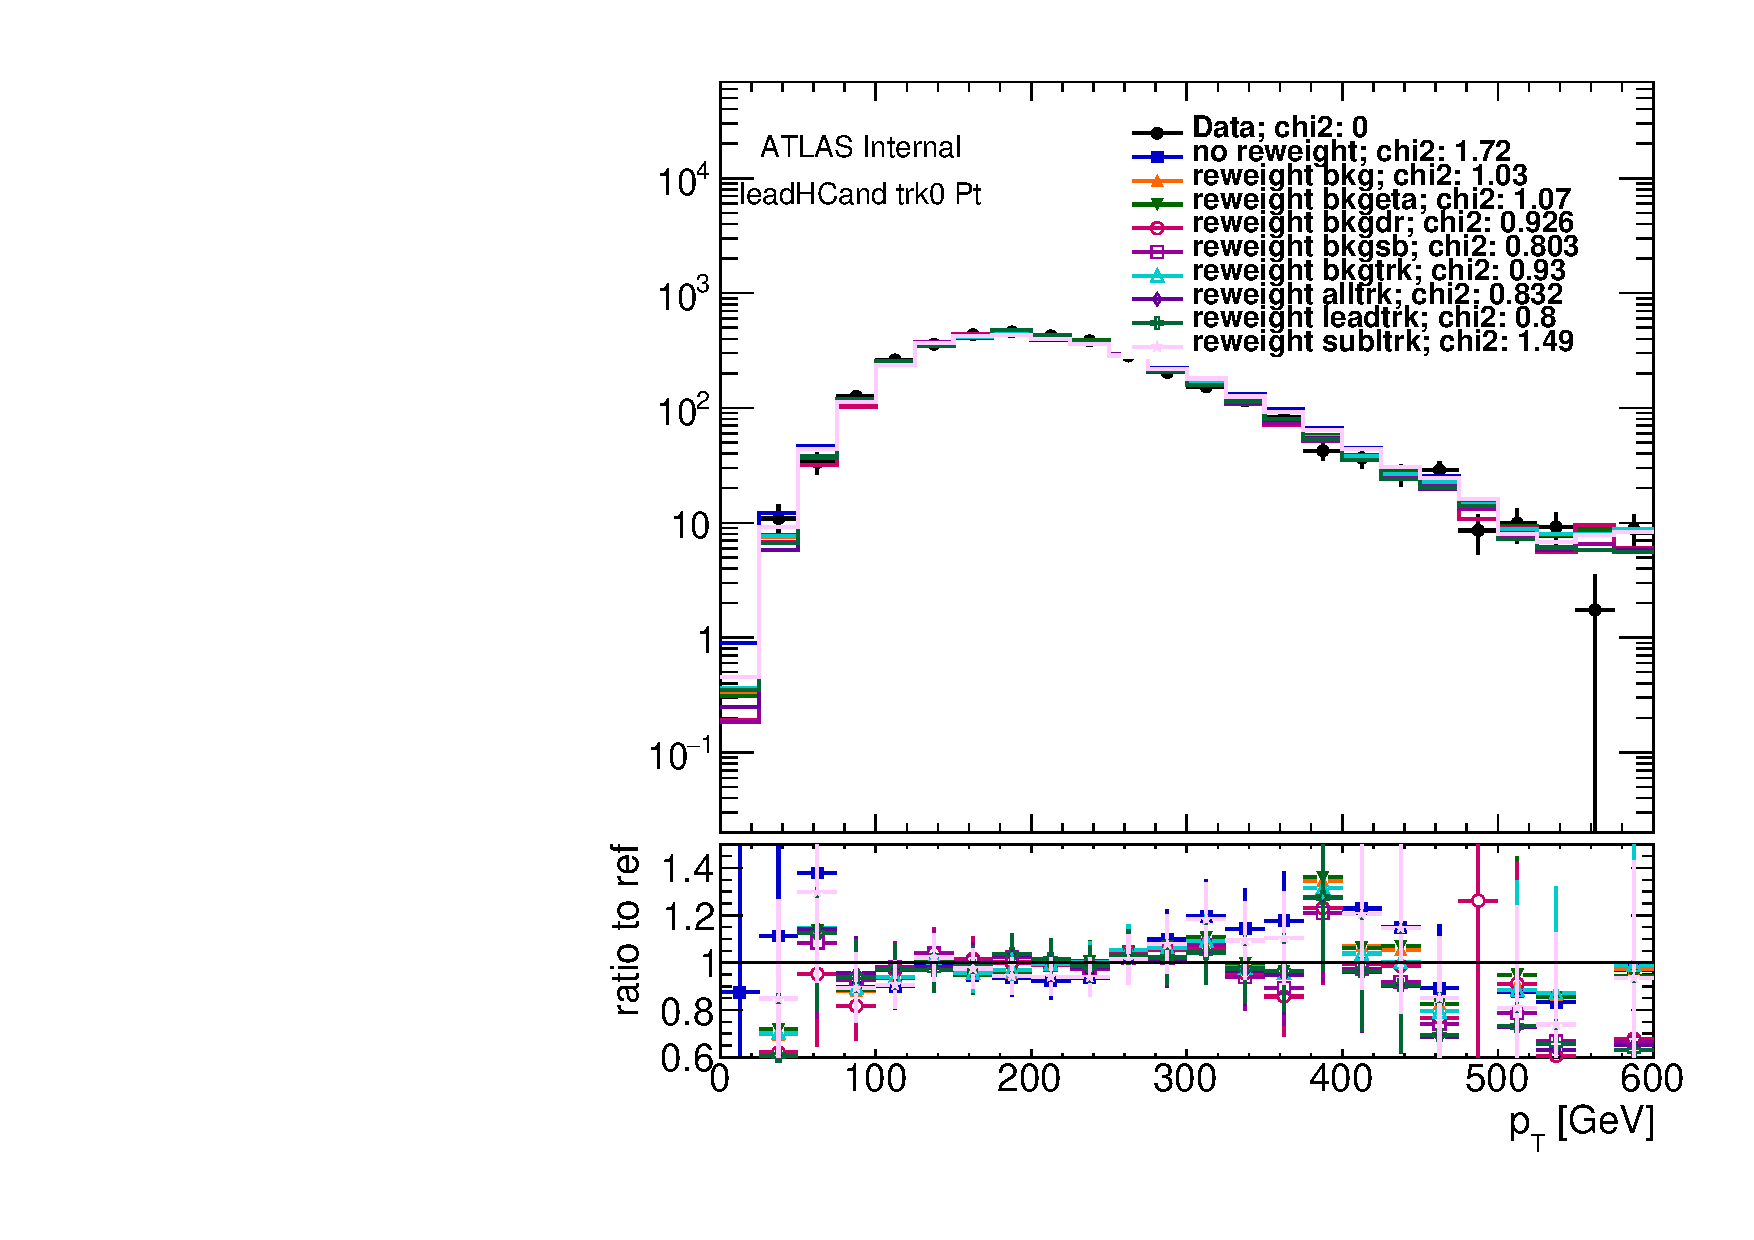
\includegraphics[width=0.24\textwidth,angle=-90]{figures/boosted/AppendixReweight/Compare/Data_ThreeTag_Sideband_directcompare_leadHCand_trk0_Pt_1.pdf}
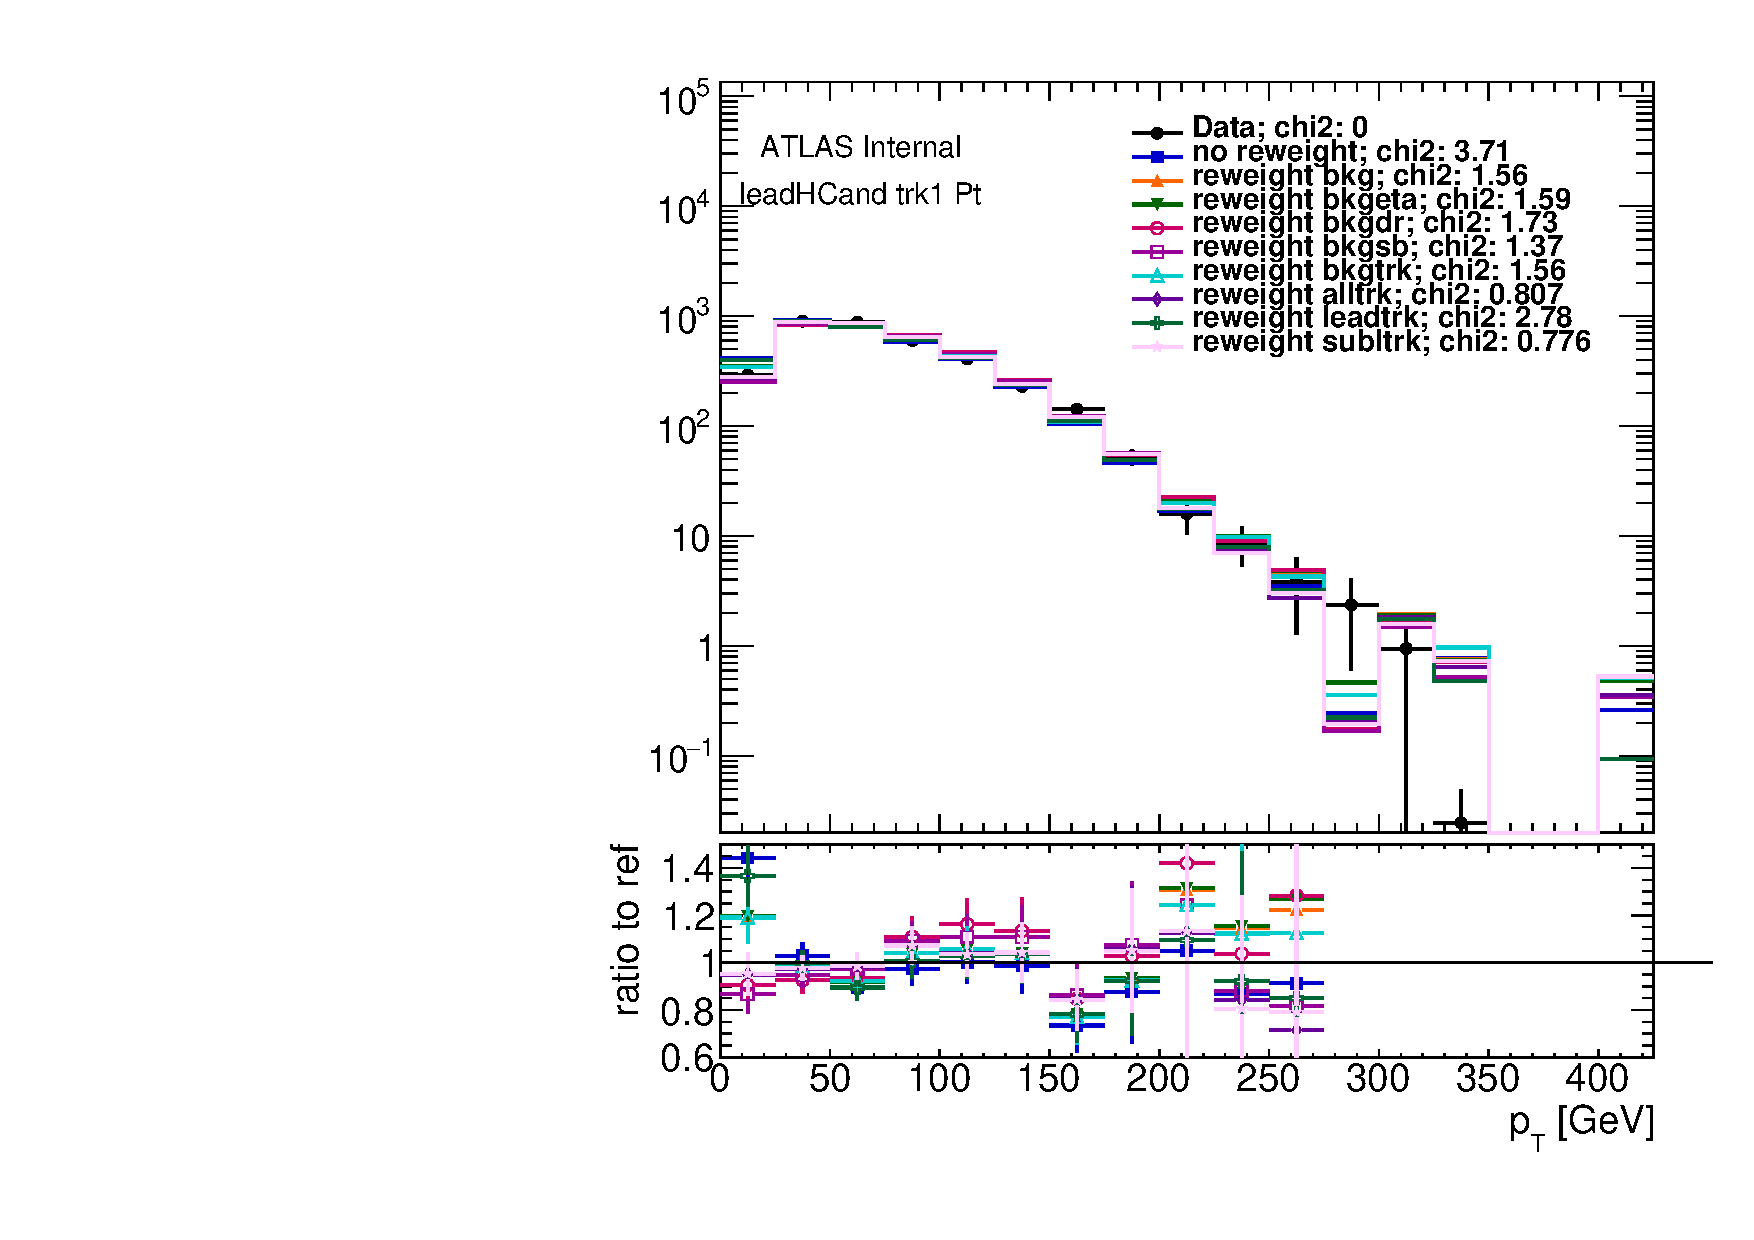
\includegraphics[width=0.24\textwidth,angle=-90]{figures/boosted/AppendixReweight/Compare/Data_ThreeTag_Sideband_directcompare_leadHCand_trk1_Pt_1.pdf}
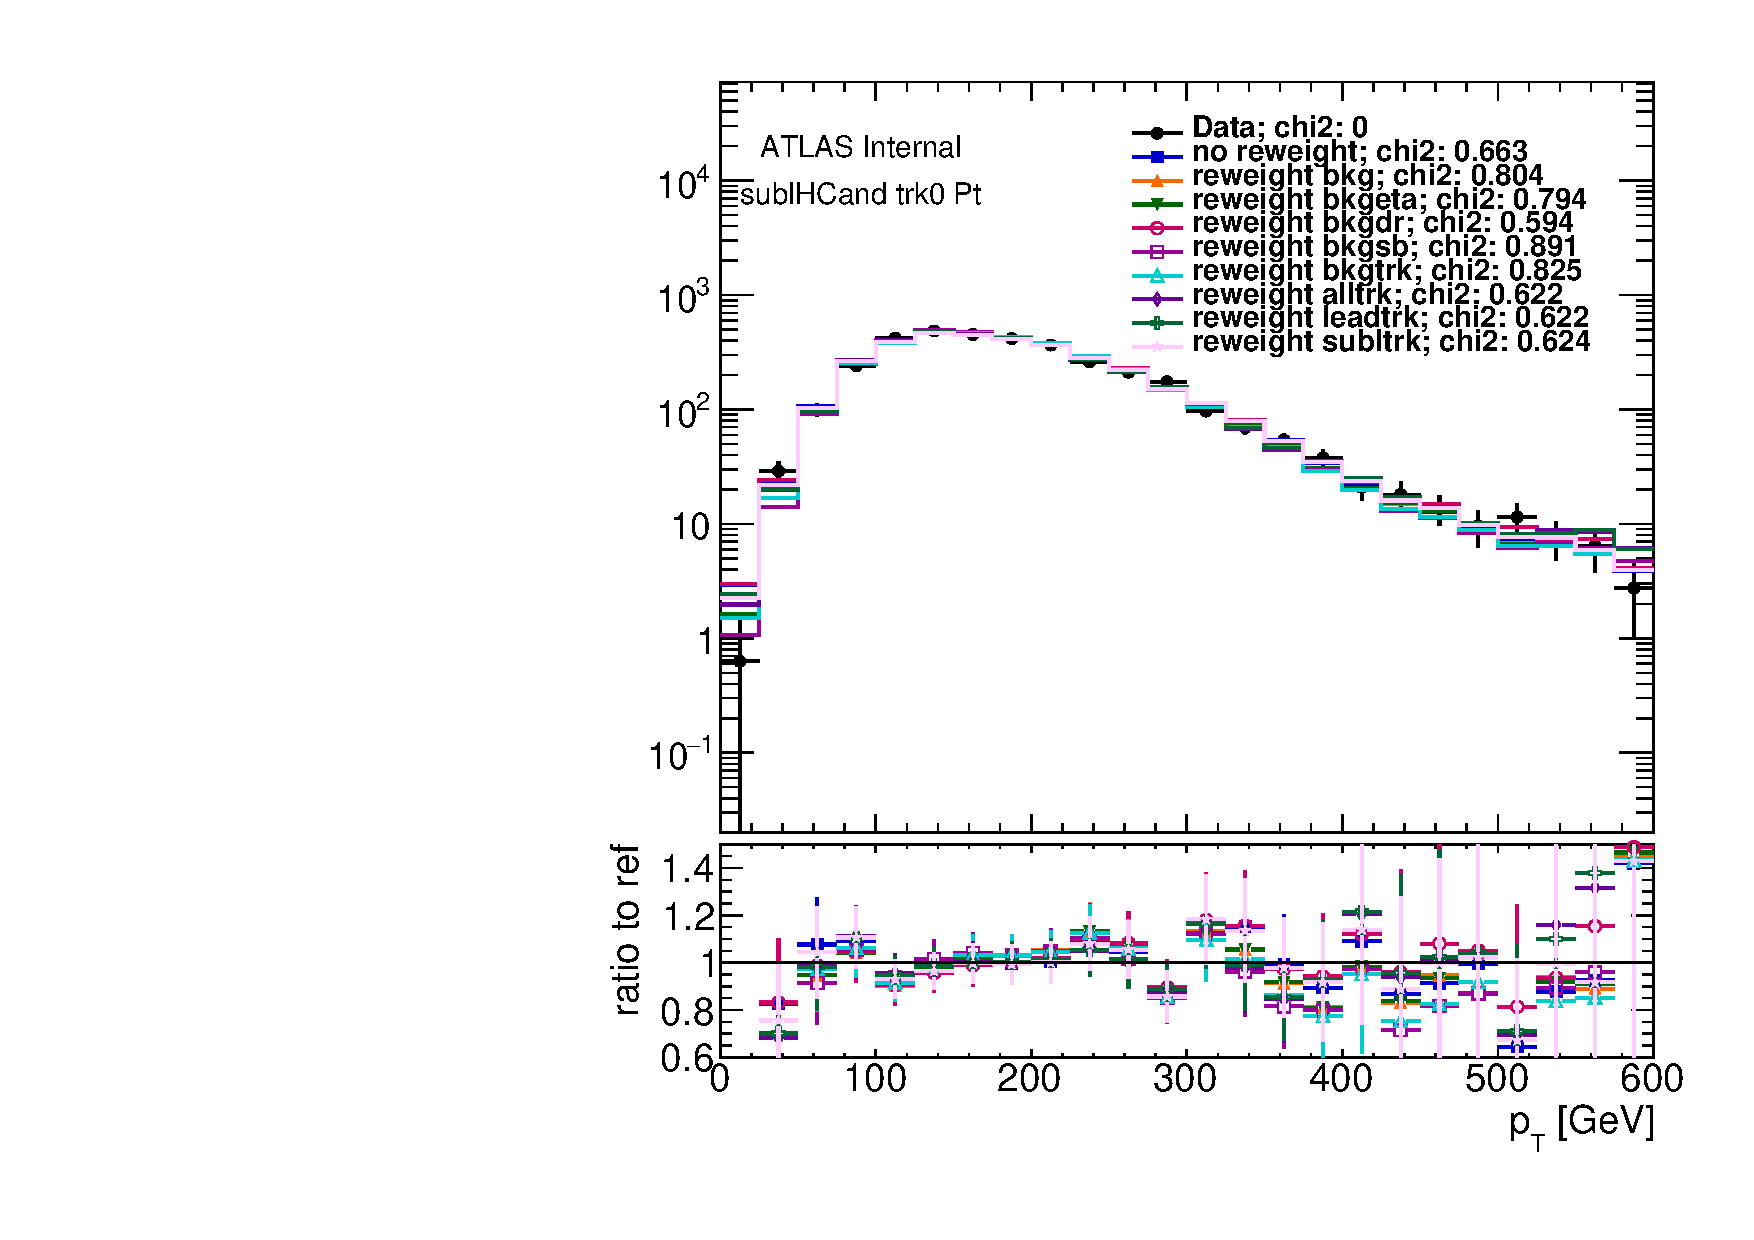
\includegraphics[width=0.24\textwidth,angle=-90]{figures/boosted/AppendixReweight/Compare/Data_ThreeTag_Sideband_directcompare_sublHCand_trk0_Pt_1.pdf}
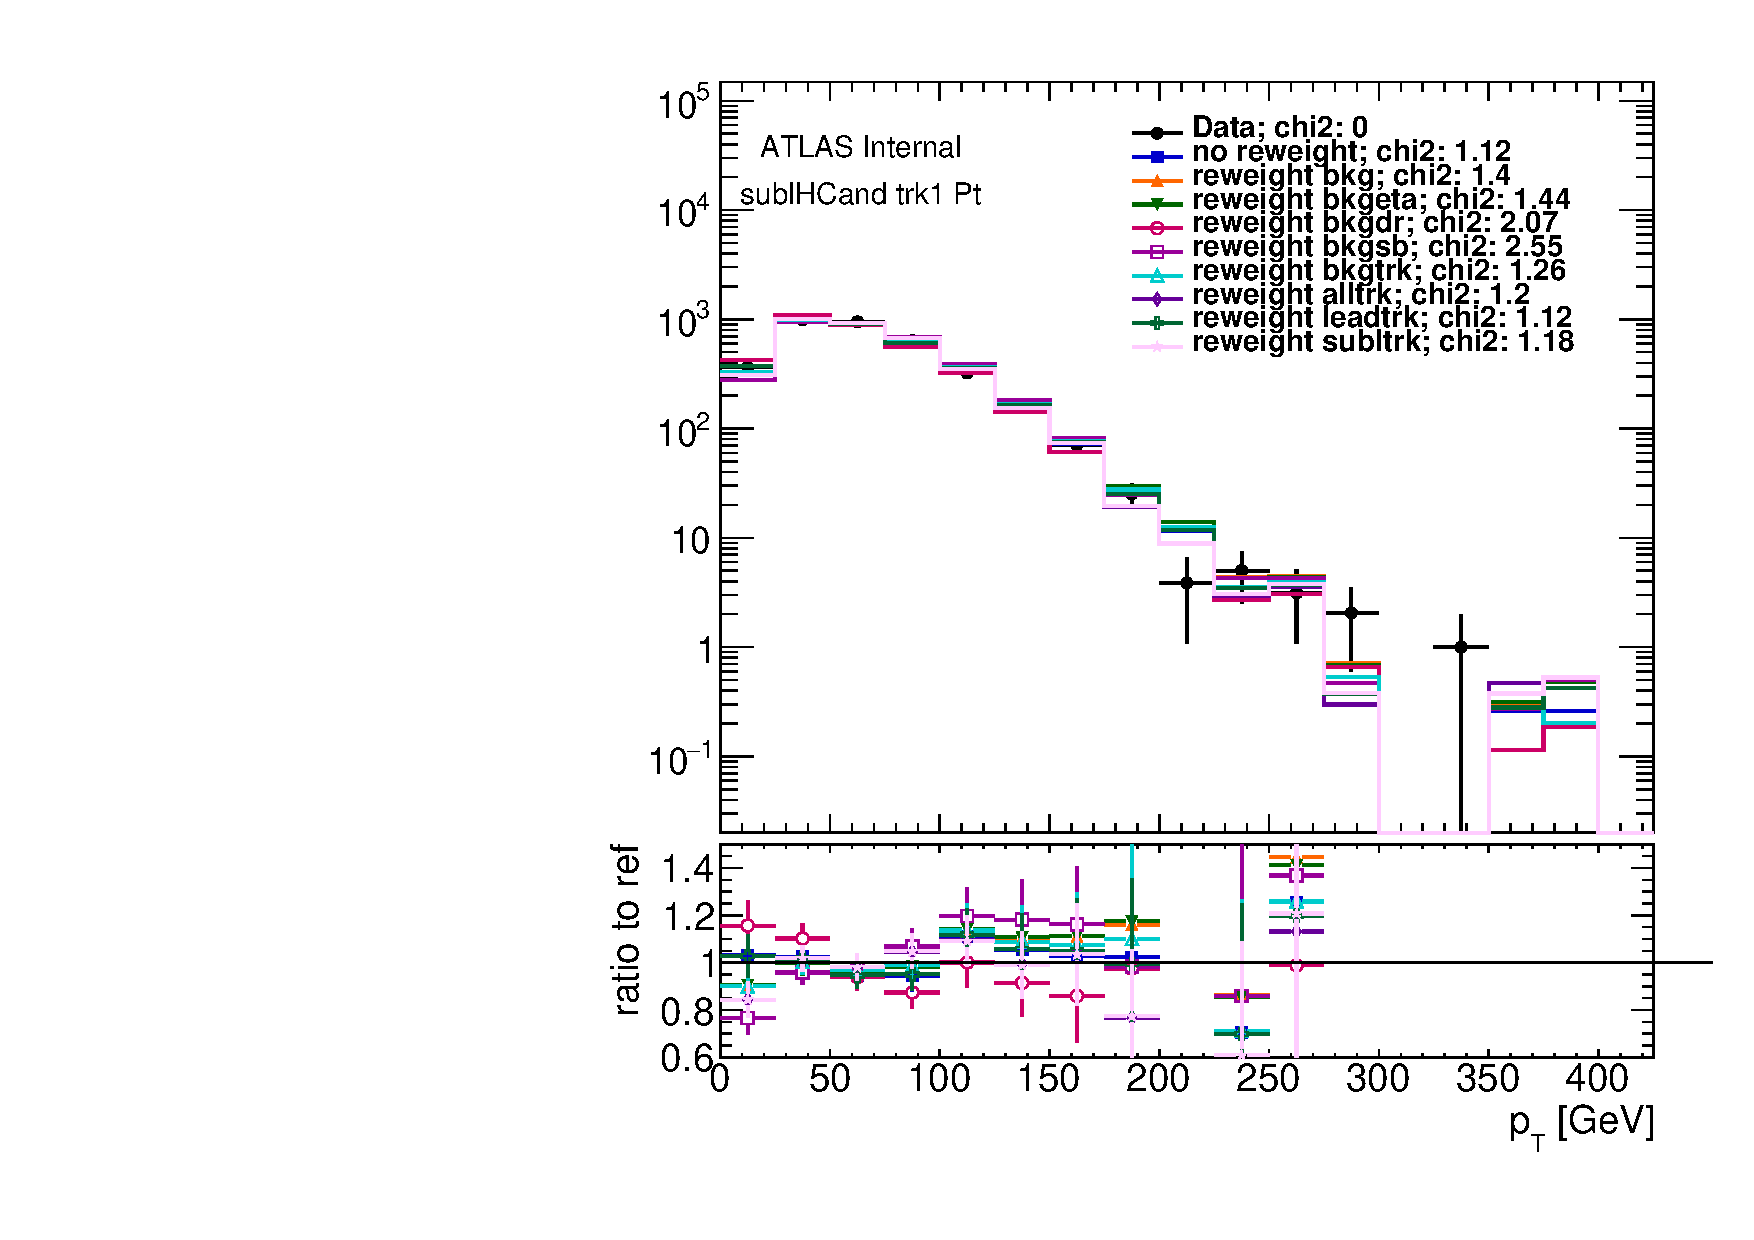
\includegraphics[width=0.24\textwidth,angle=-90]{figures/boosted/AppendixReweight/Compare/Data_ThreeTag_Sideband_directcompare_sublHCand_trk1_Pt_1.pdf}\\
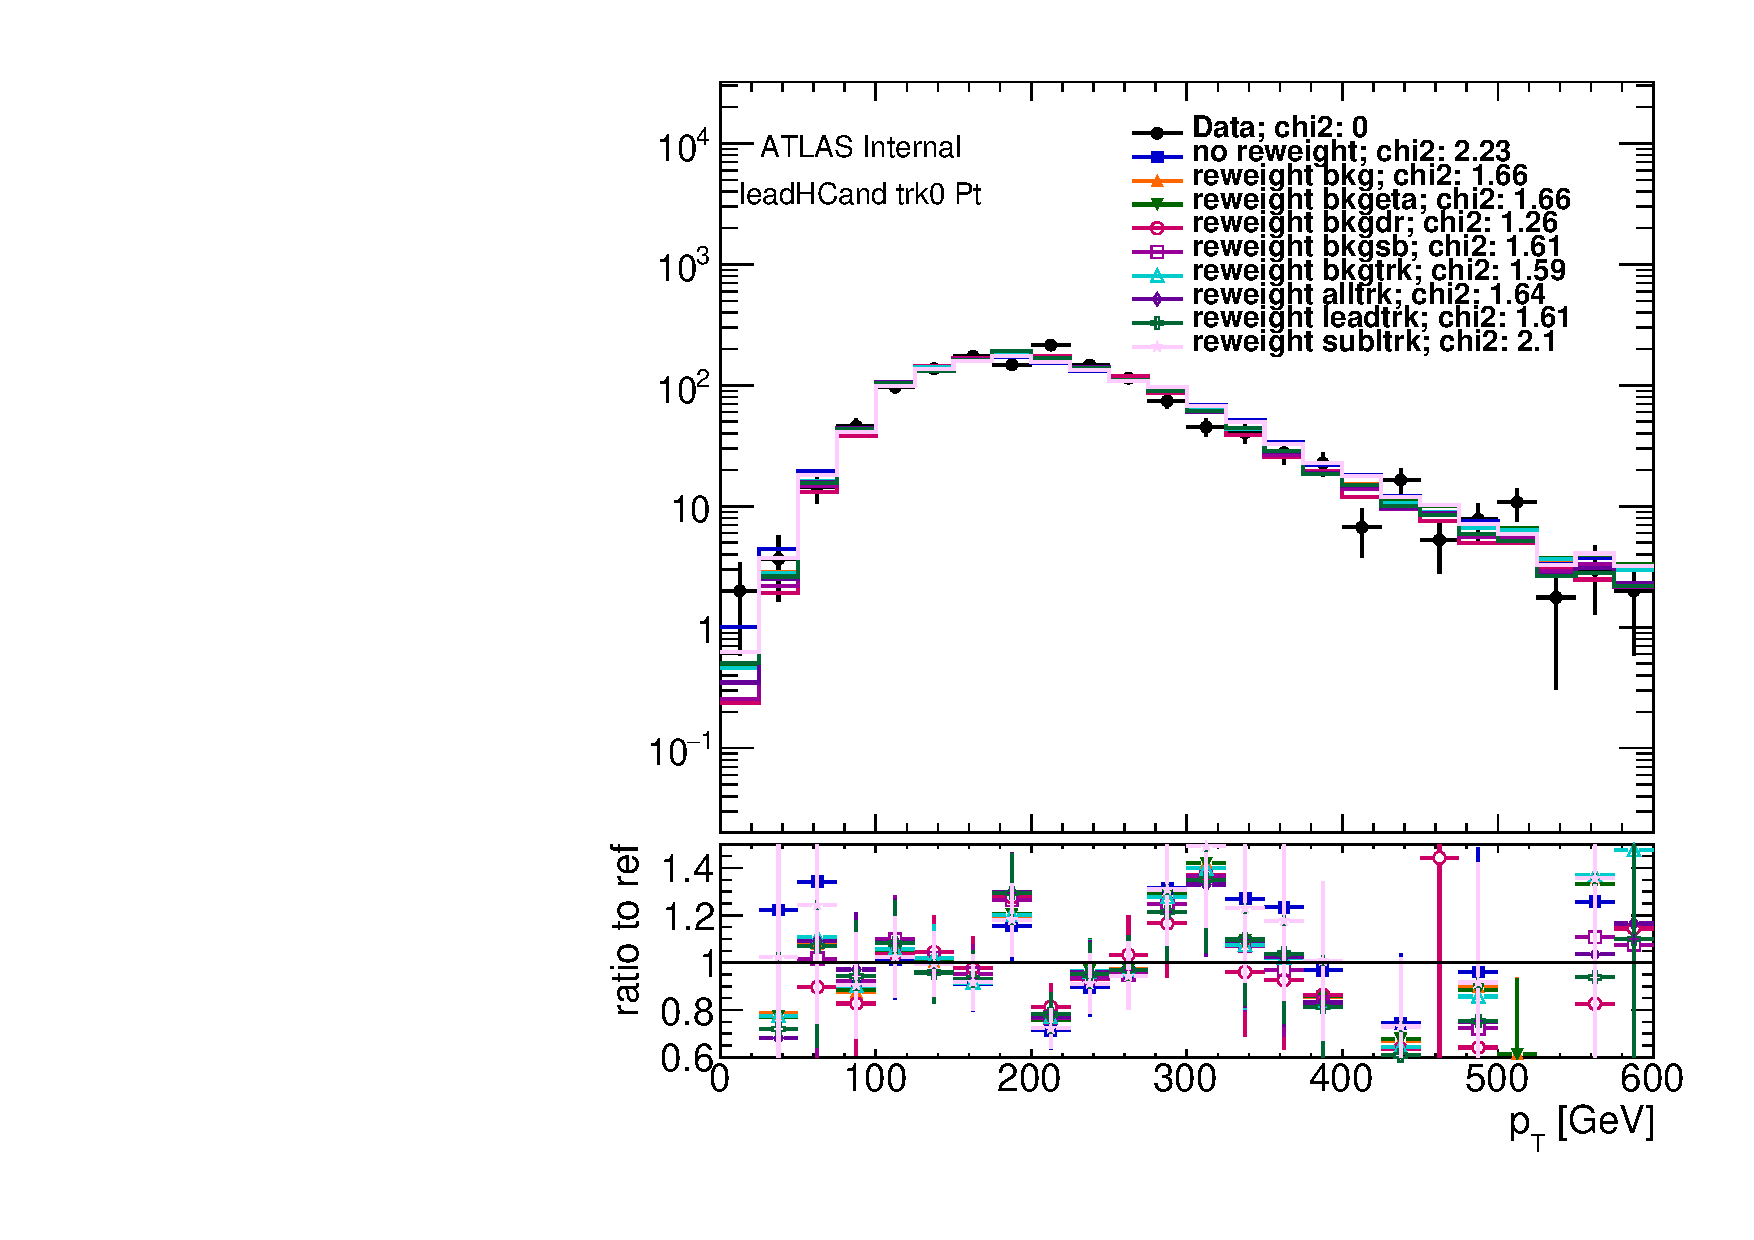
\includegraphics[width=0.24\textwidth,angle=-90]{figures/boosted/AppendixReweight/Compare/Data_ThreeTag_Control_directcompare_leadHCand_trk0_Pt_1.pdf}
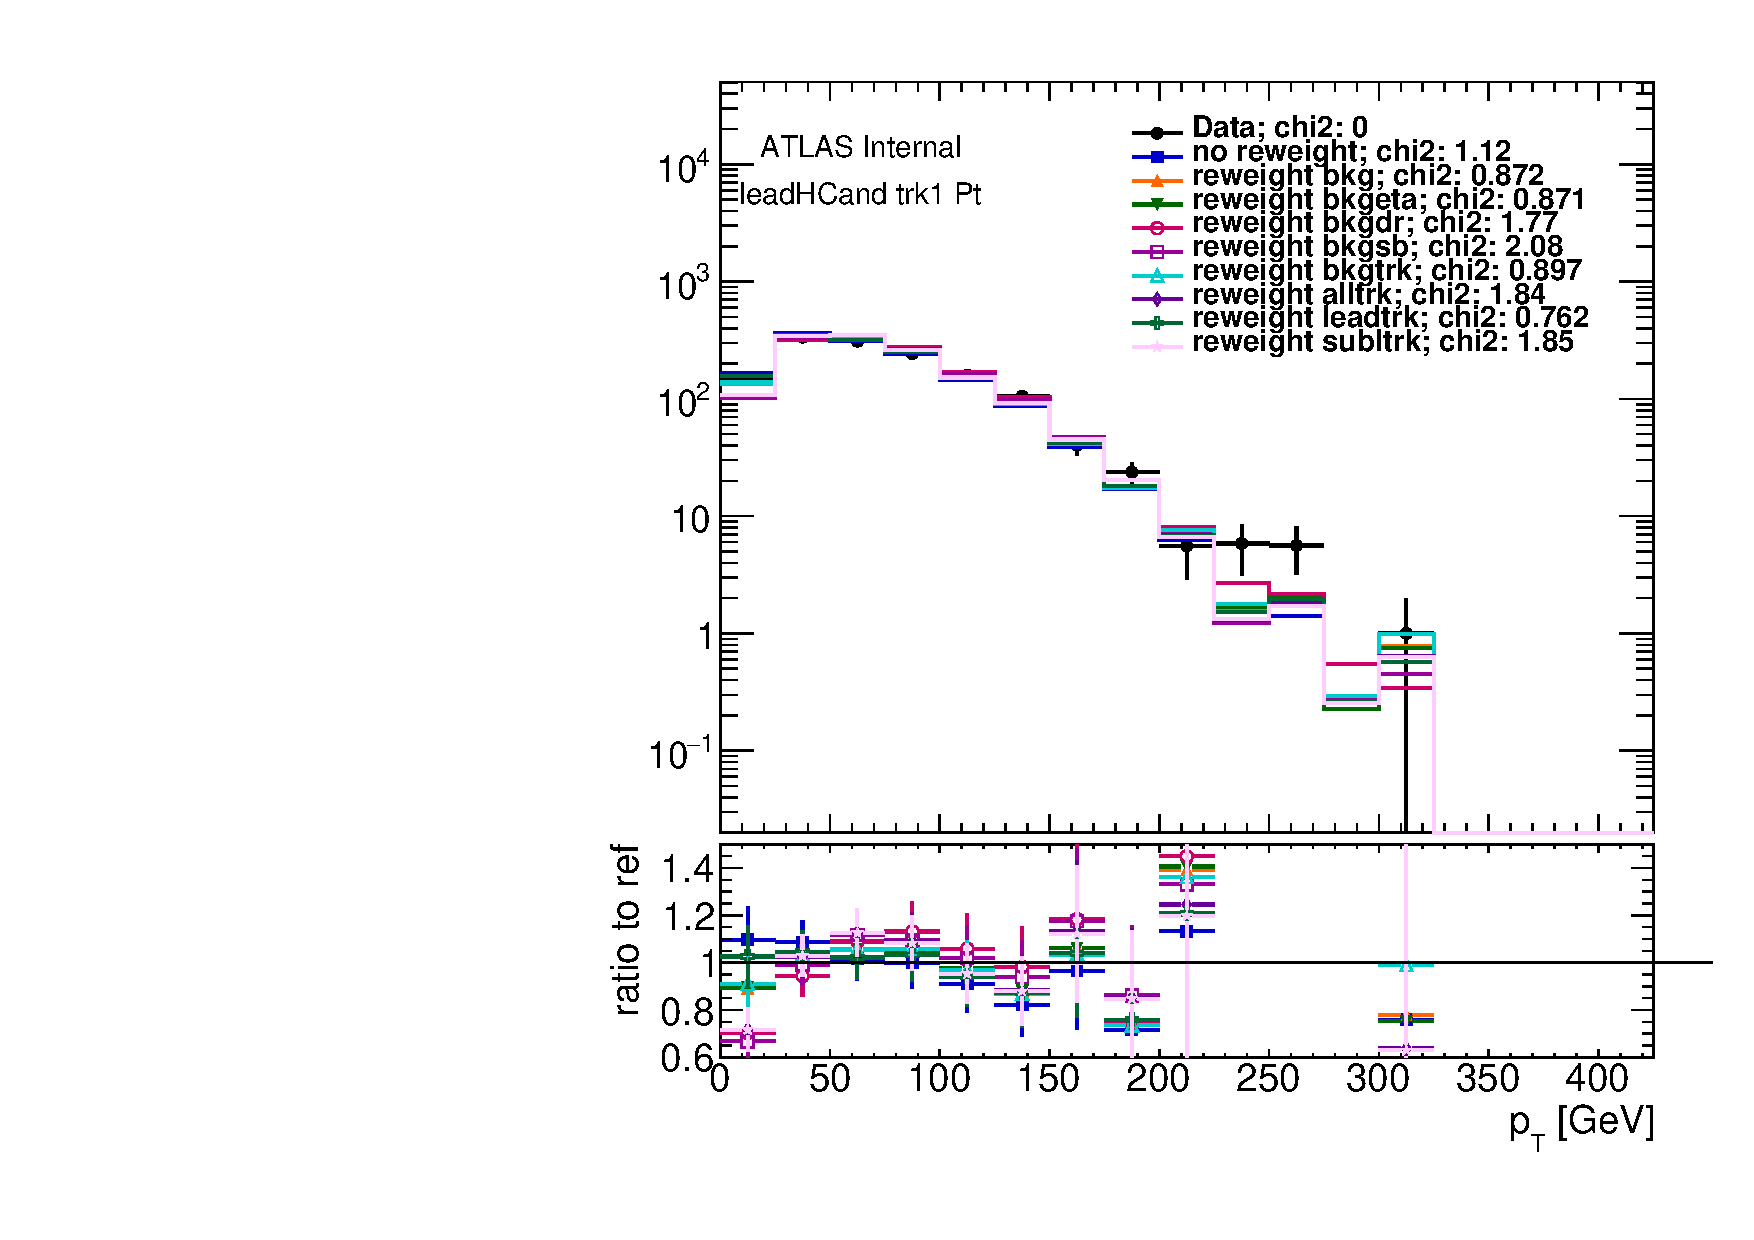
\includegraphics[width=0.24\textwidth,angle=-90]{figures/boosted/AppendixReweight/Compare/Data_ThreeTag_Control_directcompare_leadHCand_trk1_Pt_1.pdf}
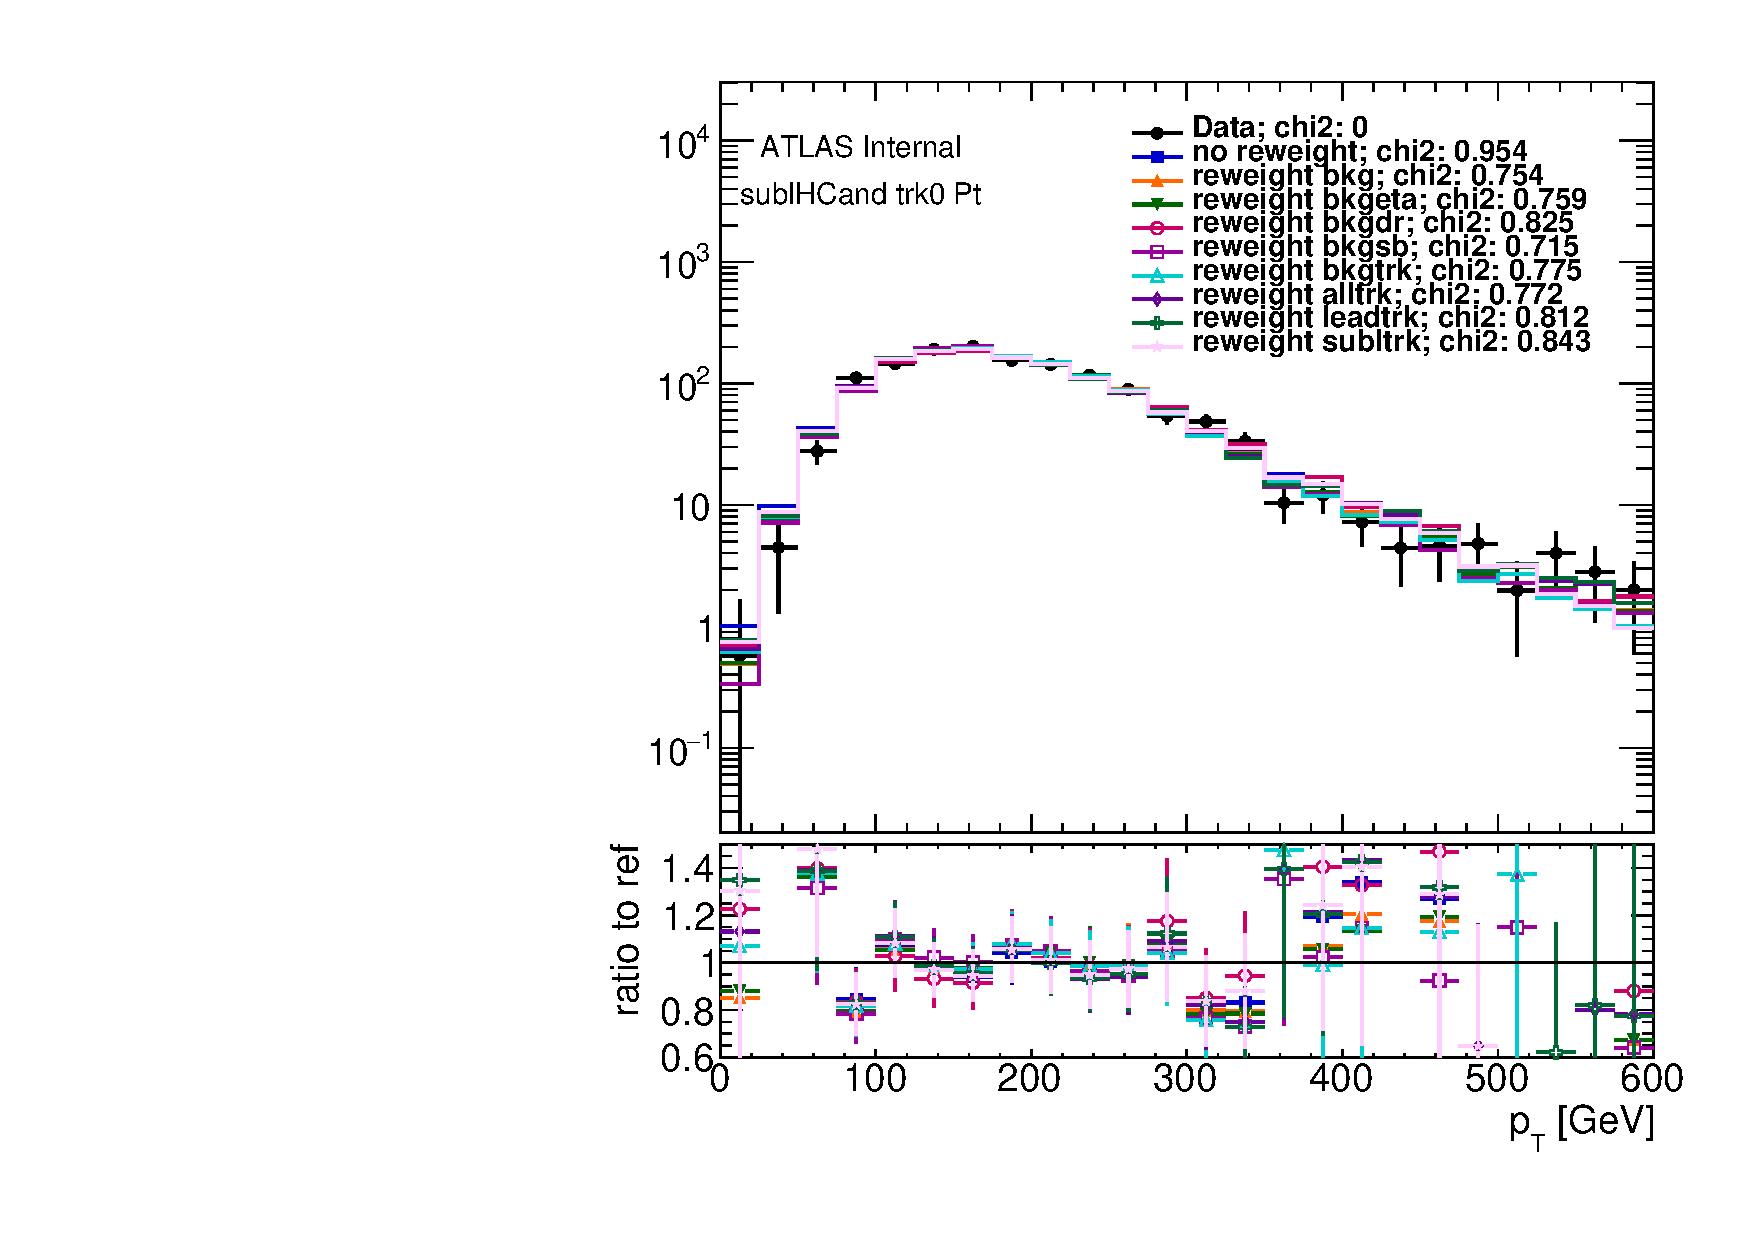
\includegraphics[width=0.24\textwidth,angle=-90]{figures/boosted/AppendixReweight/Compare/Data_ThreeTag_Control_directcompare_sublHCand_trk0_Pt_1.pdf}
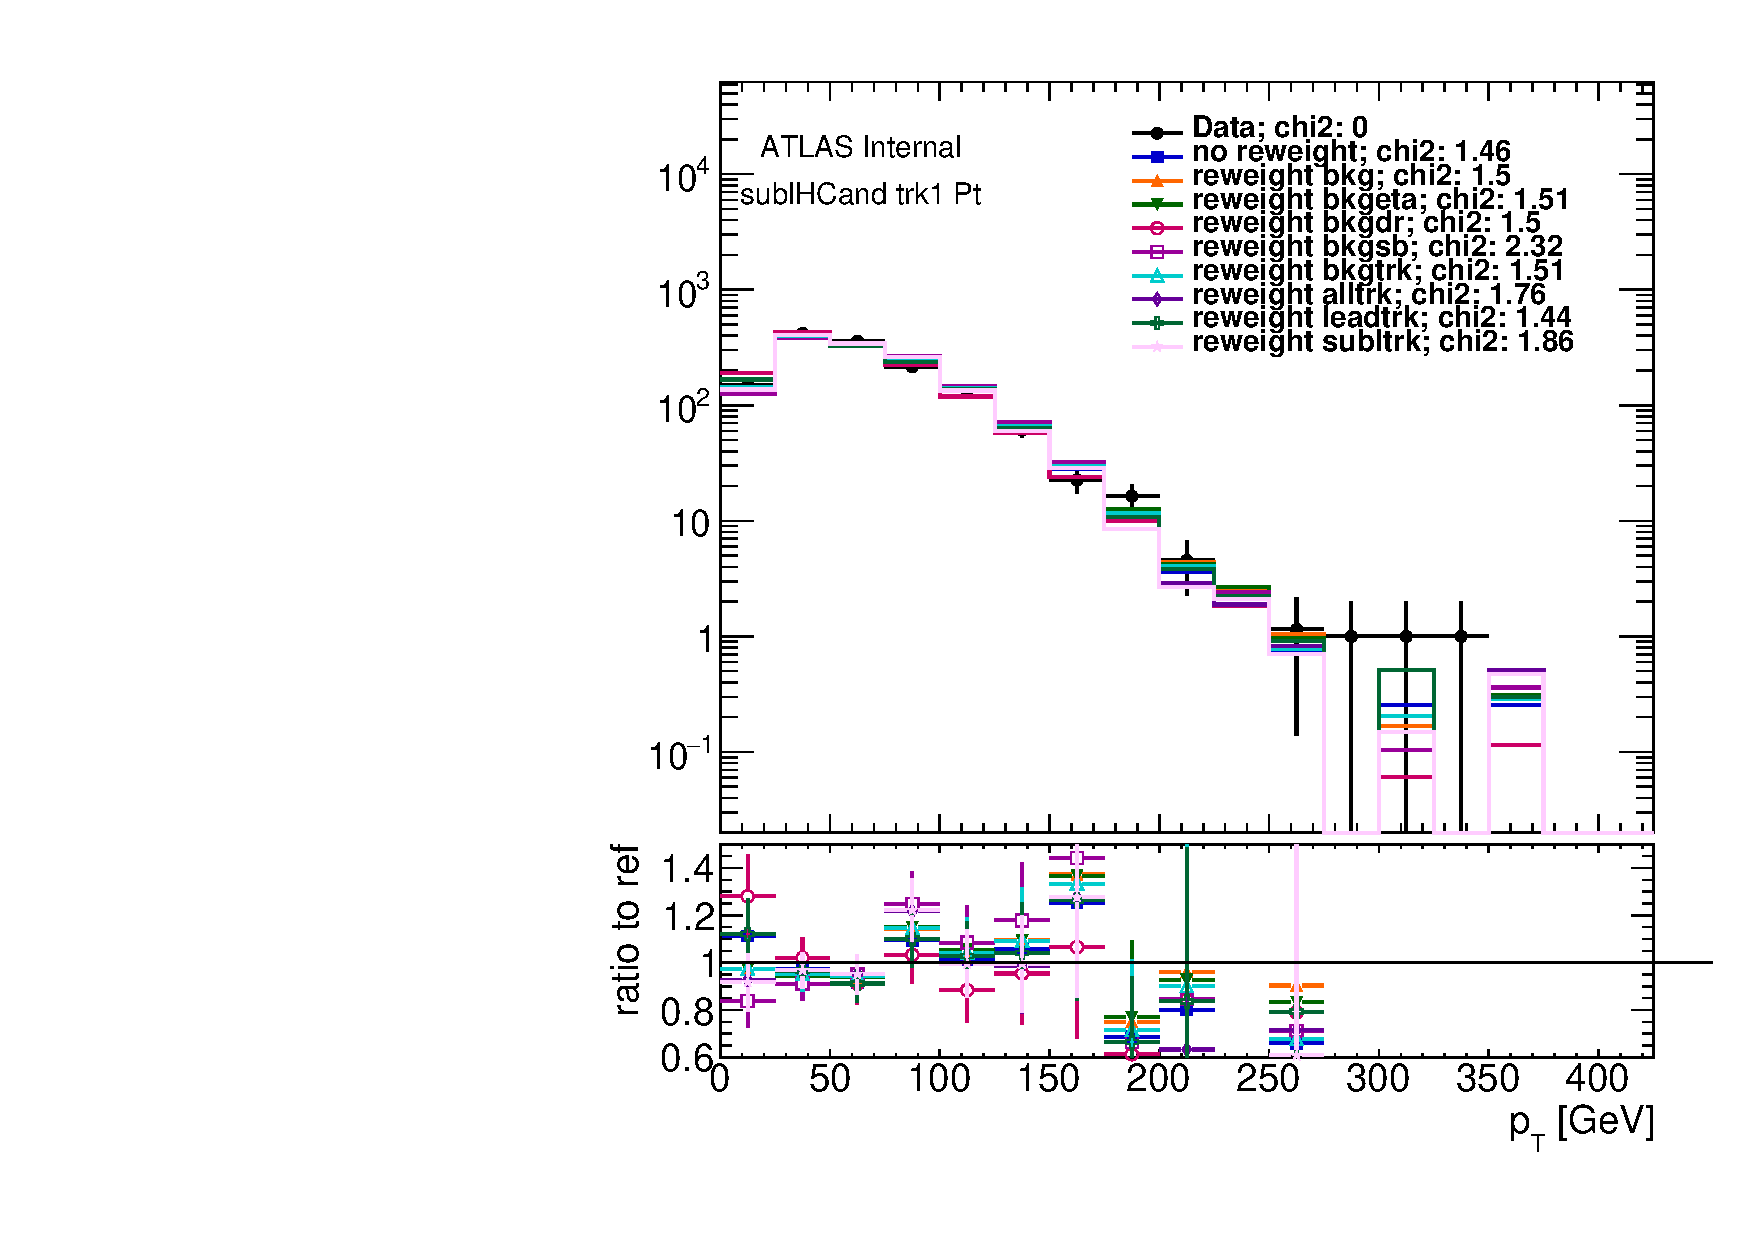
\includegraphics[width=0.24\textwidth,angle=-90]{figures/boosted/AppendixReweight/Compare/Data_ThreeTag_Control_directcompare_sublHCand_trk1_Pt_1.pdf}\\
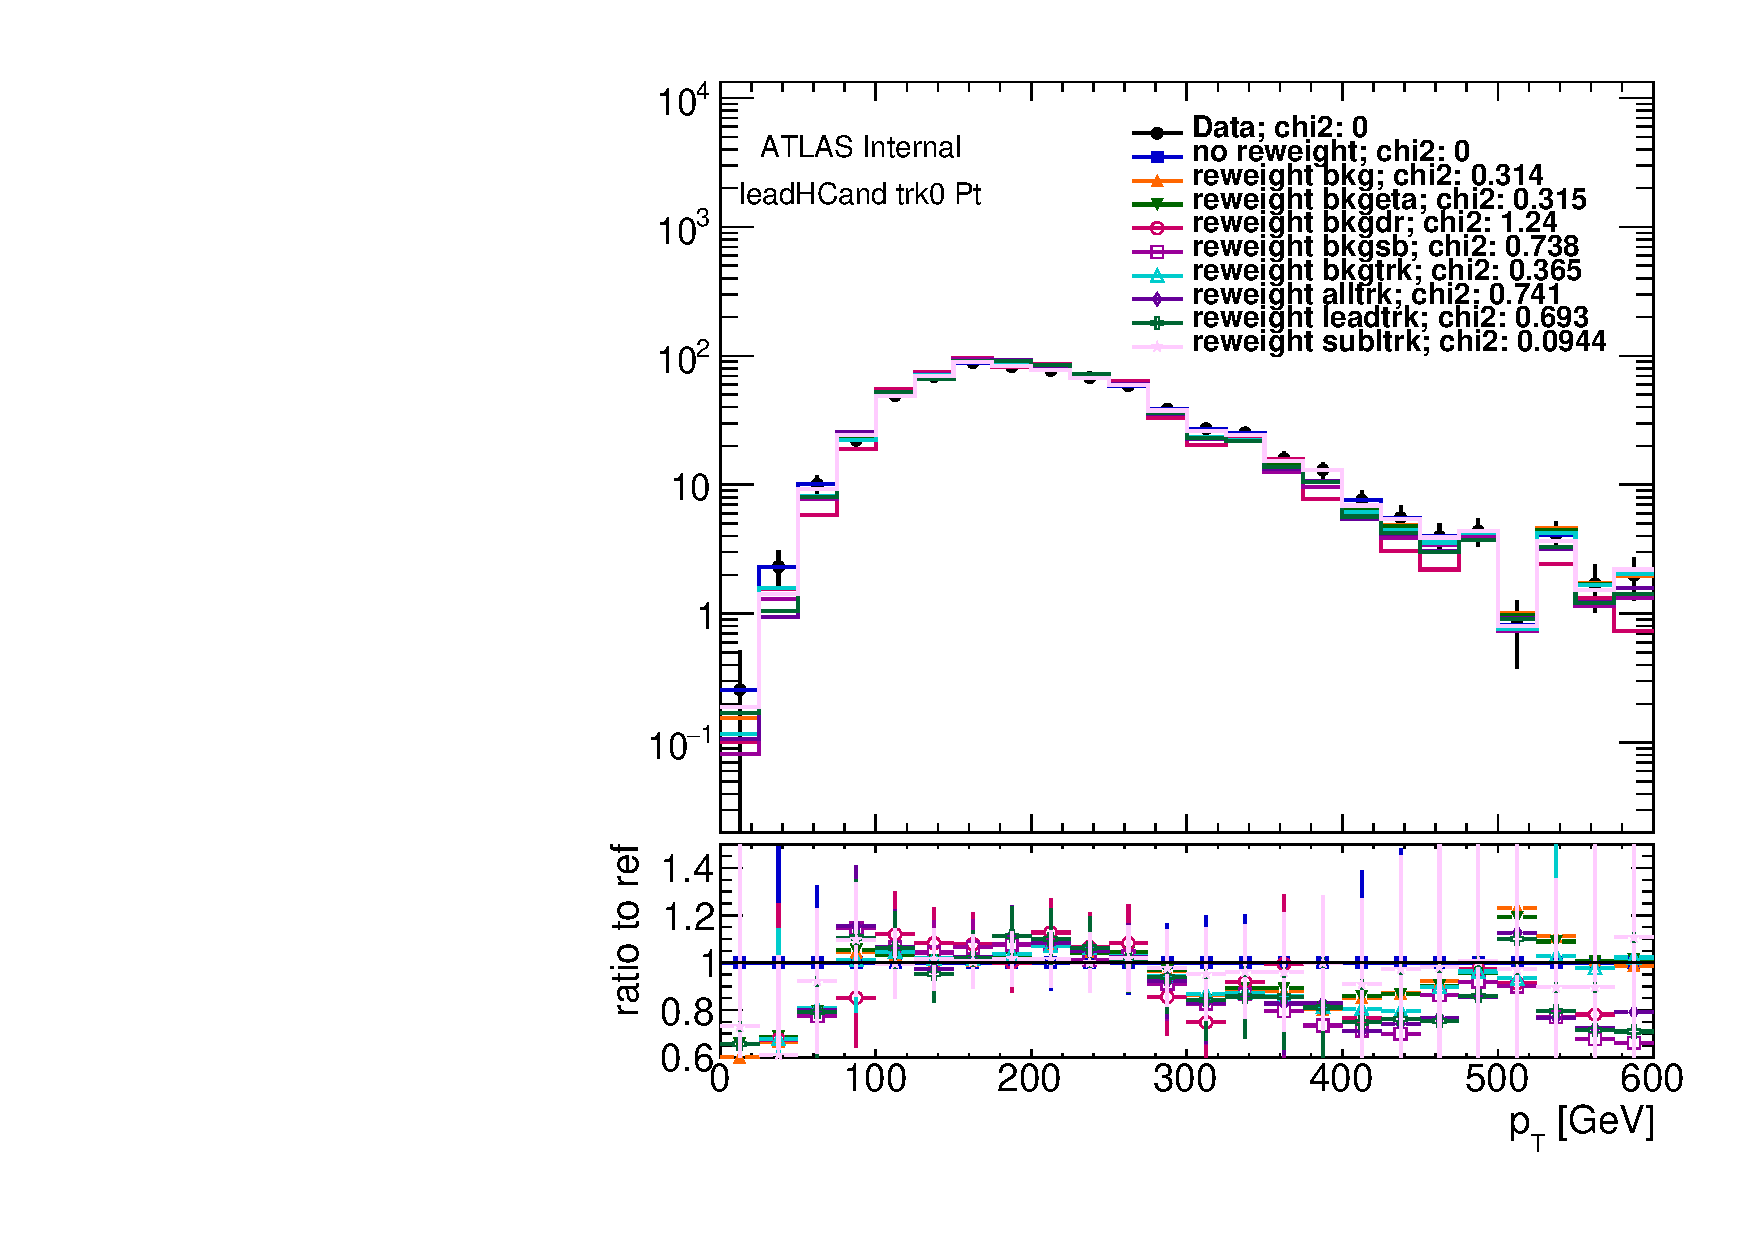
\includegraphics[width=0.24\textwidth,angle=-90]{figures/boosted/AppendixReweight/Compare/Data_ThreeTag_Signal_directcompare_leadHCand_trk0_Pt_1.pdf}
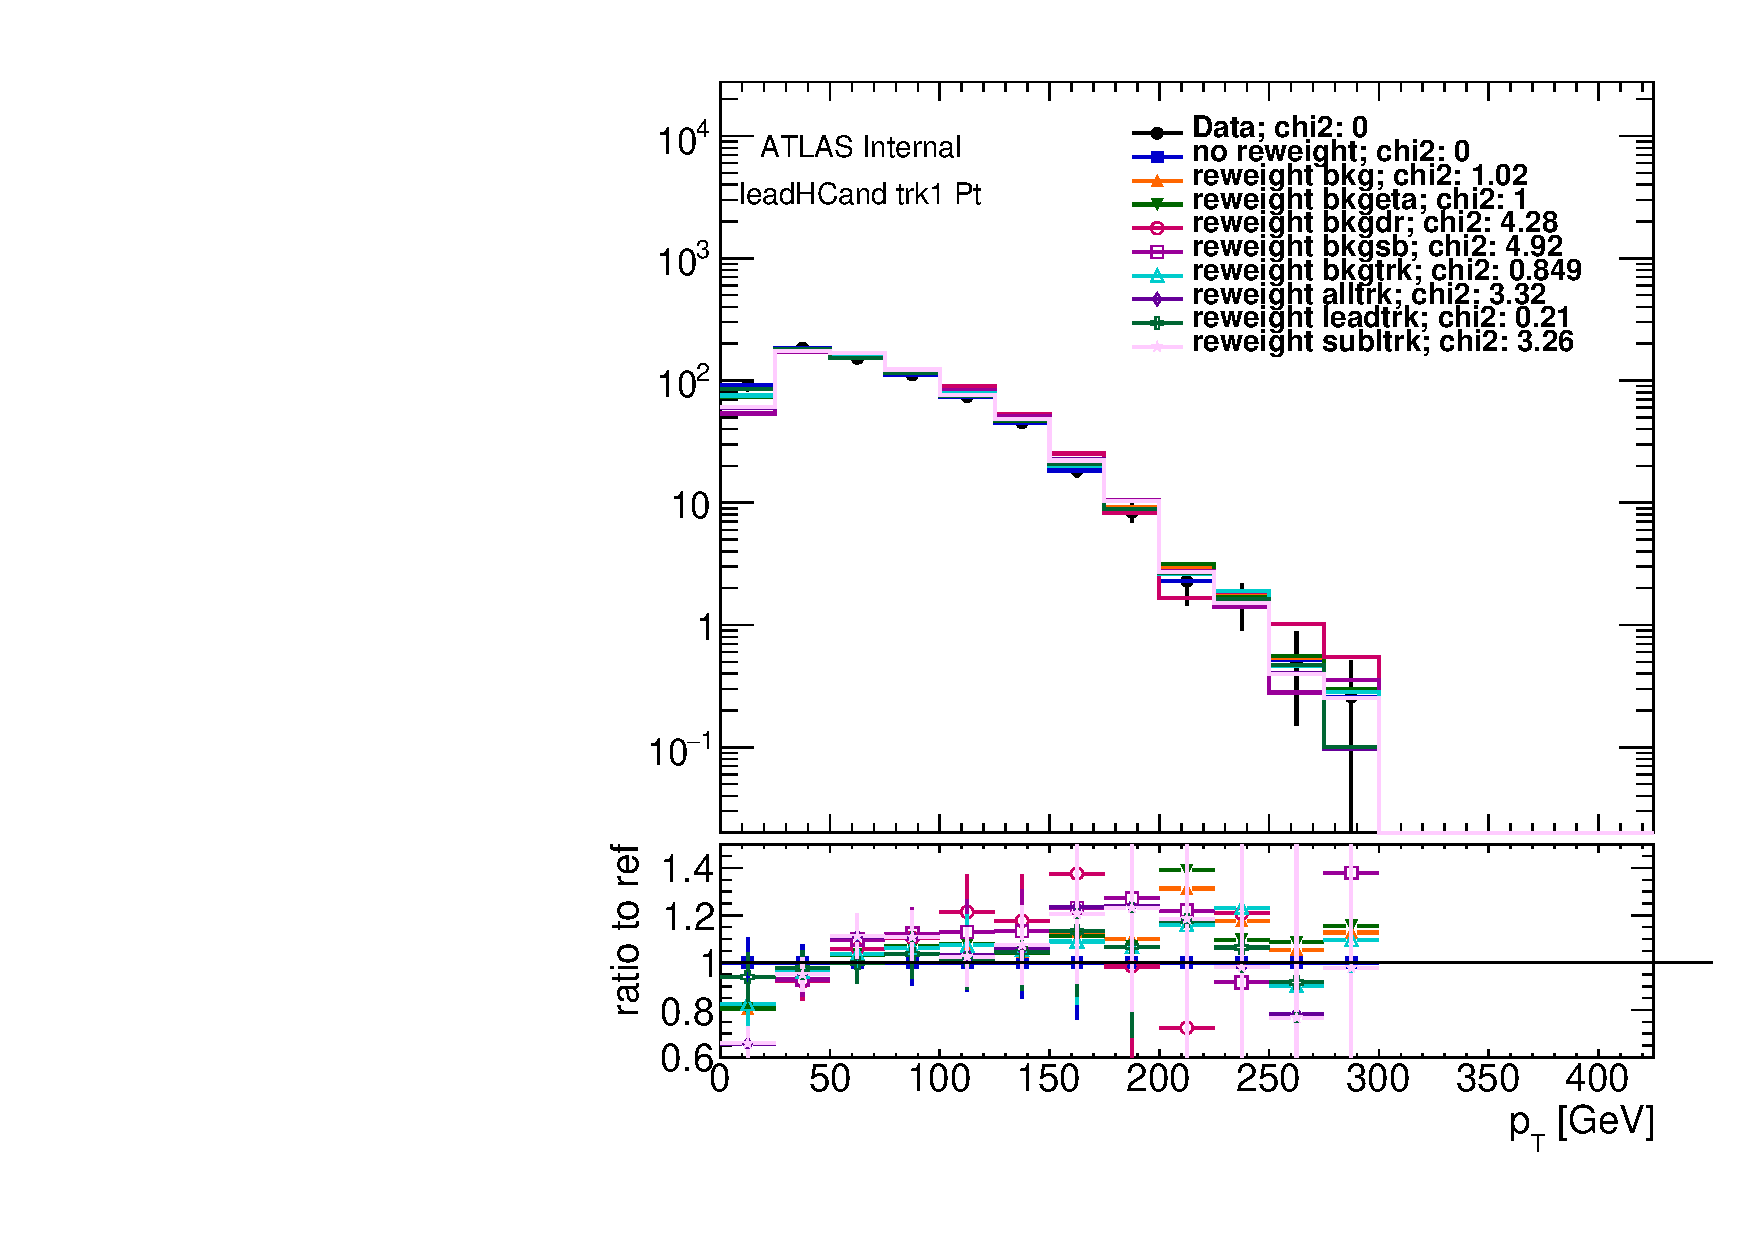
\includegraphics[width=0.24\textwidth,angle=-90]{figures/boosted/AppendixReweight/Compare/Data_ThreeTag_Signal_directcompare_leadHCand_trk1_Pt_1.pdf}
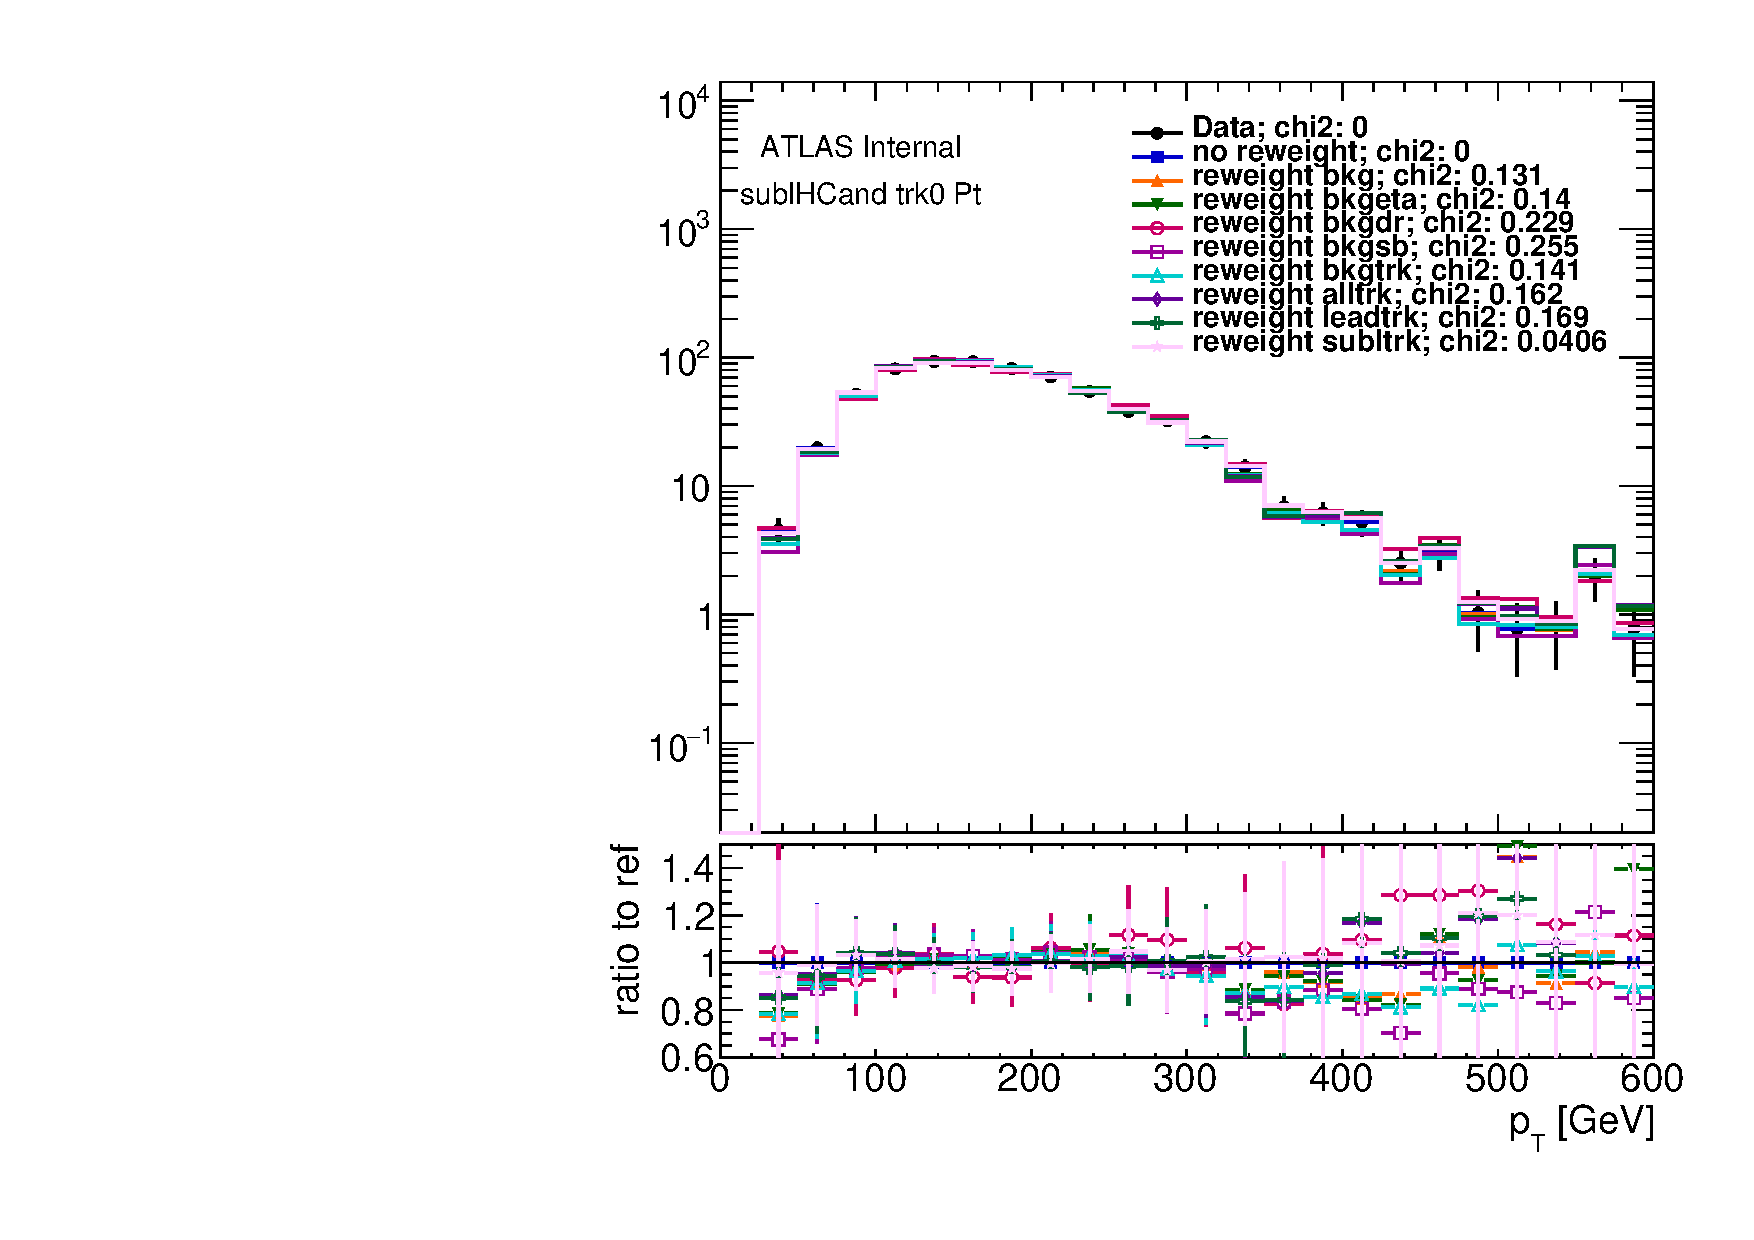
\includegraphics[width=0.24\textwidth,angle=-90]{figures/boosted/AppendixReweight/Compare/Data_ThreeTag_Signal_directcompare_sublHCand_trk0_Pt_1.pdf}
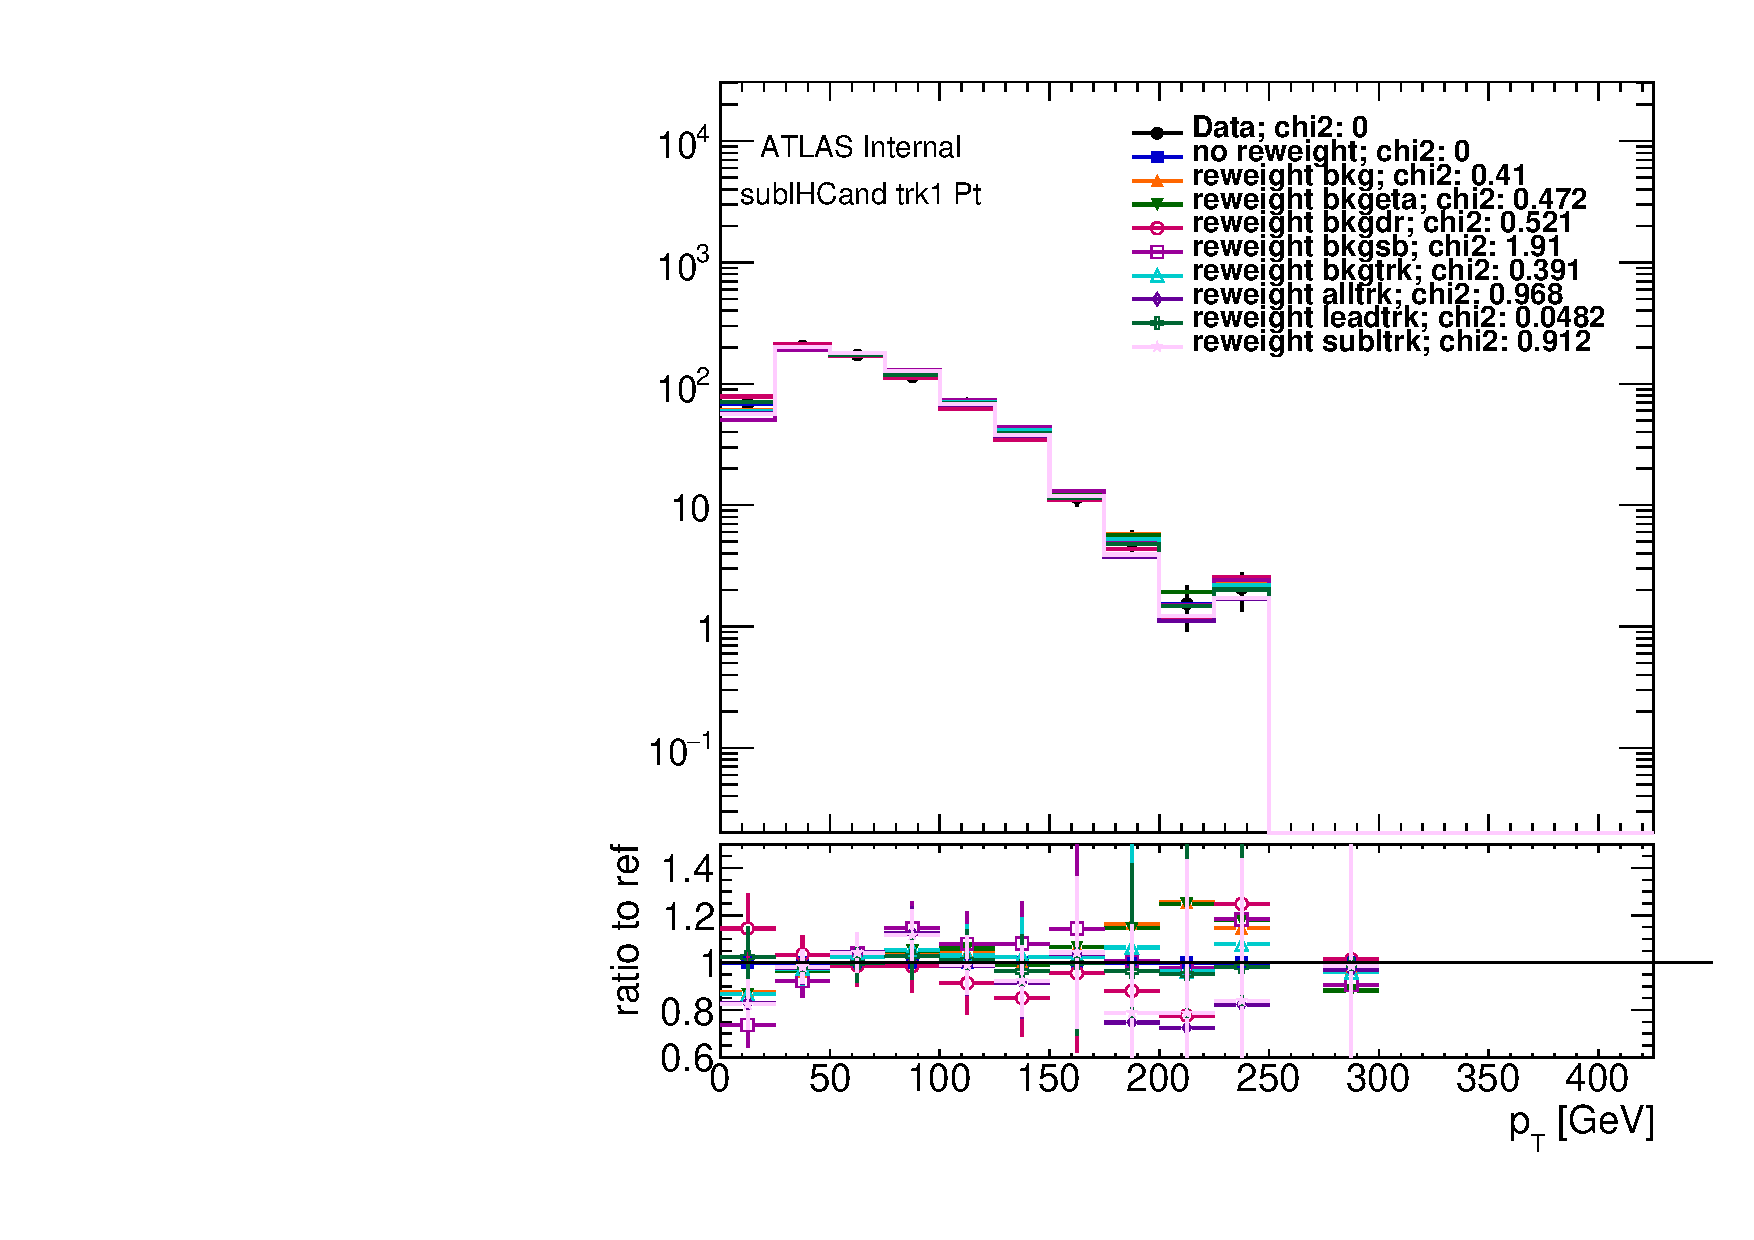
\includegraphics[width=0.24\textwidth,angle=-90]{figures/boosted/AppendixReweight/Compare/Data_ThreeTag_Signal_directcompare_sublHCand_trk1_Pt_1.pdf}\\
\caption{Reweighted $3b$ Sideband (top)/Control (middle)/Signal(bottom) region predictions comaprison, for leading Higgs Candidate leading trackjet \pt (first column),  leading Higgs Candidate subleading trackjet \pt (second column), subleading Higgs Candidate leading trackjet \pt (third column), subleading Higgs Candidate subleading trackjet \pt (fourth column). The Signal region is blinded, where the distribution is replaced with the non-reweighted distributions.}
\label{fig:app-rw-comp-3b-trkjet}
\end{center}
\end{figure*}

\begin{figure*}[htbp!]
\begin{center}
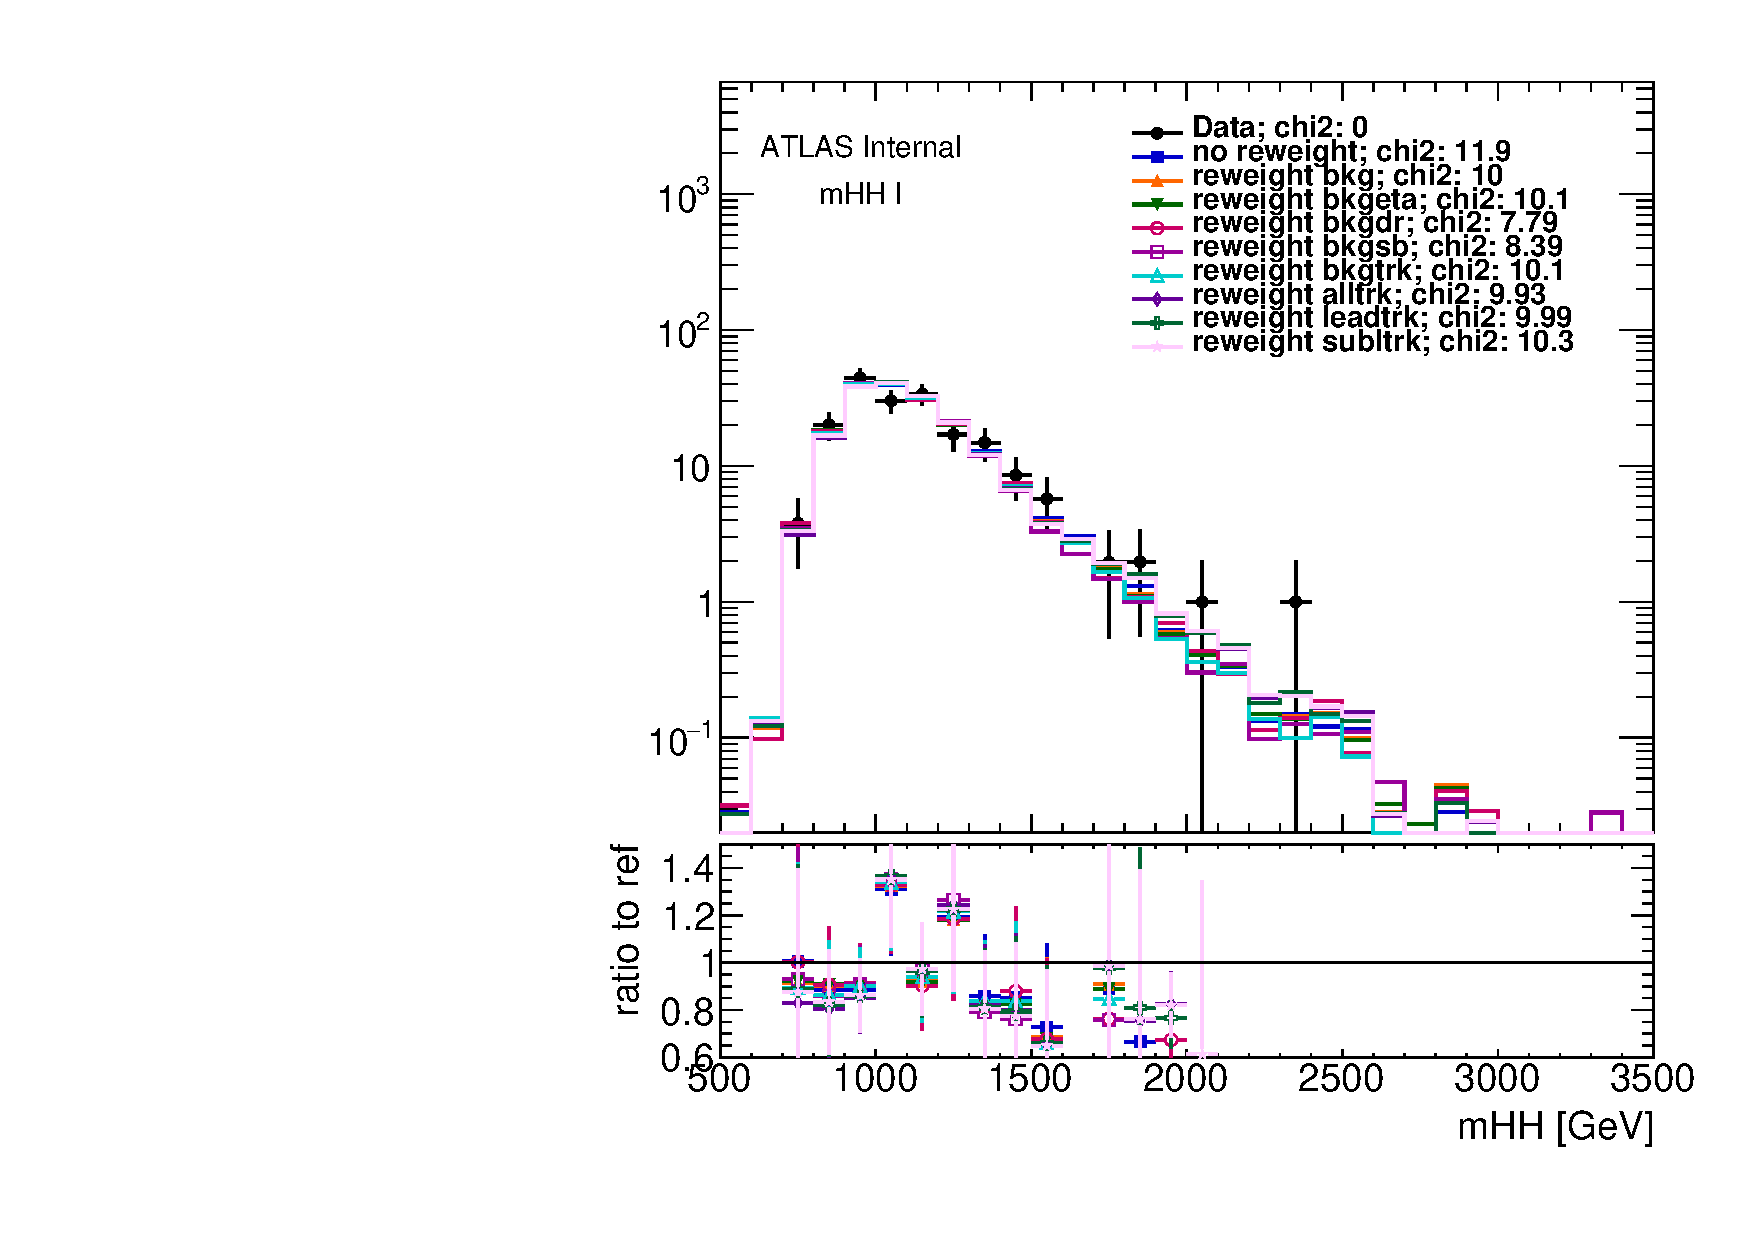
\includegraphics[width=0.4\textwidth,angle=-90]{figures/boosted/AppendixReweight/Compare/Data_FourTag_Sideband_directcompare_mHH_l_1.pdf}\\
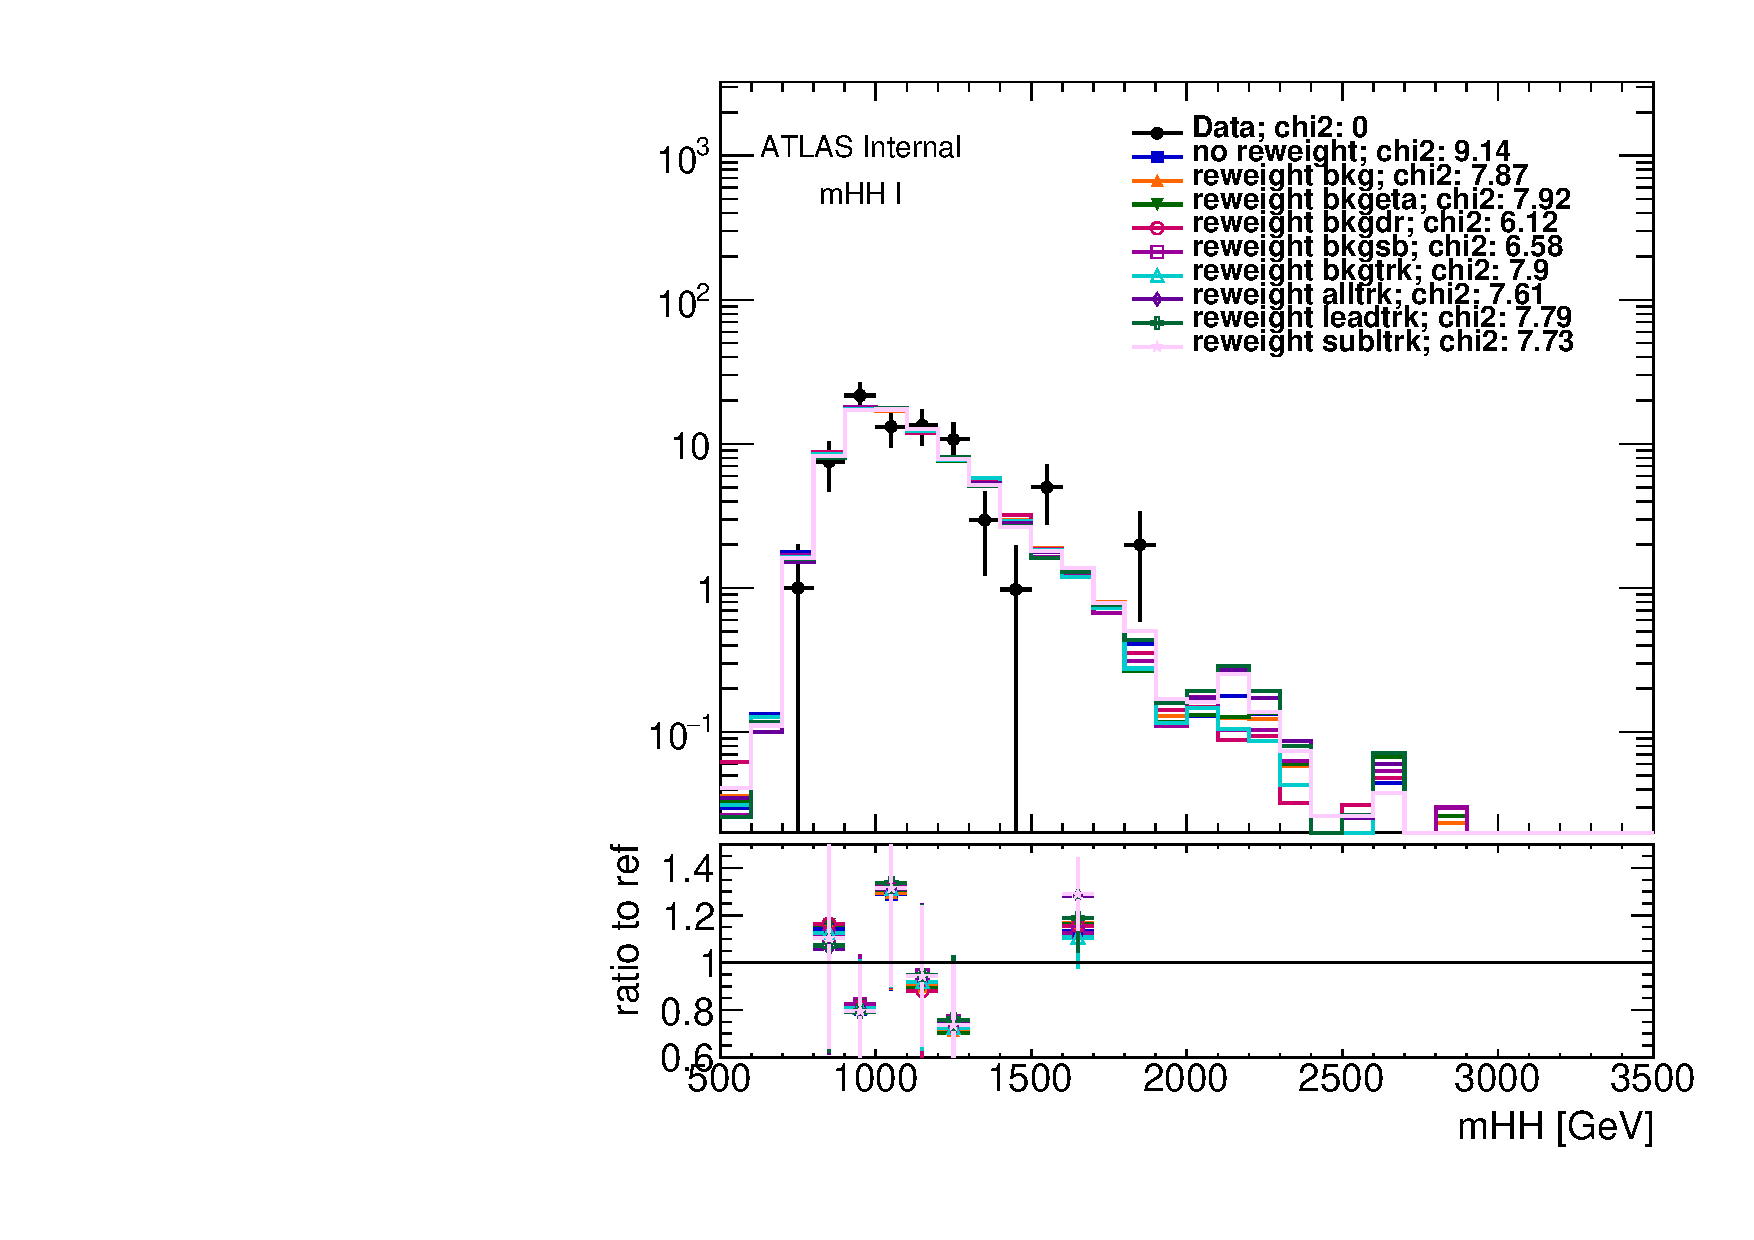
\includegraphics[width=0.4\textwidth,angle=-90]{figures/boosted/AppendixReweight/Compare/Data_FourTag_Control_directcompare_mHH_l_1.pdf}\\
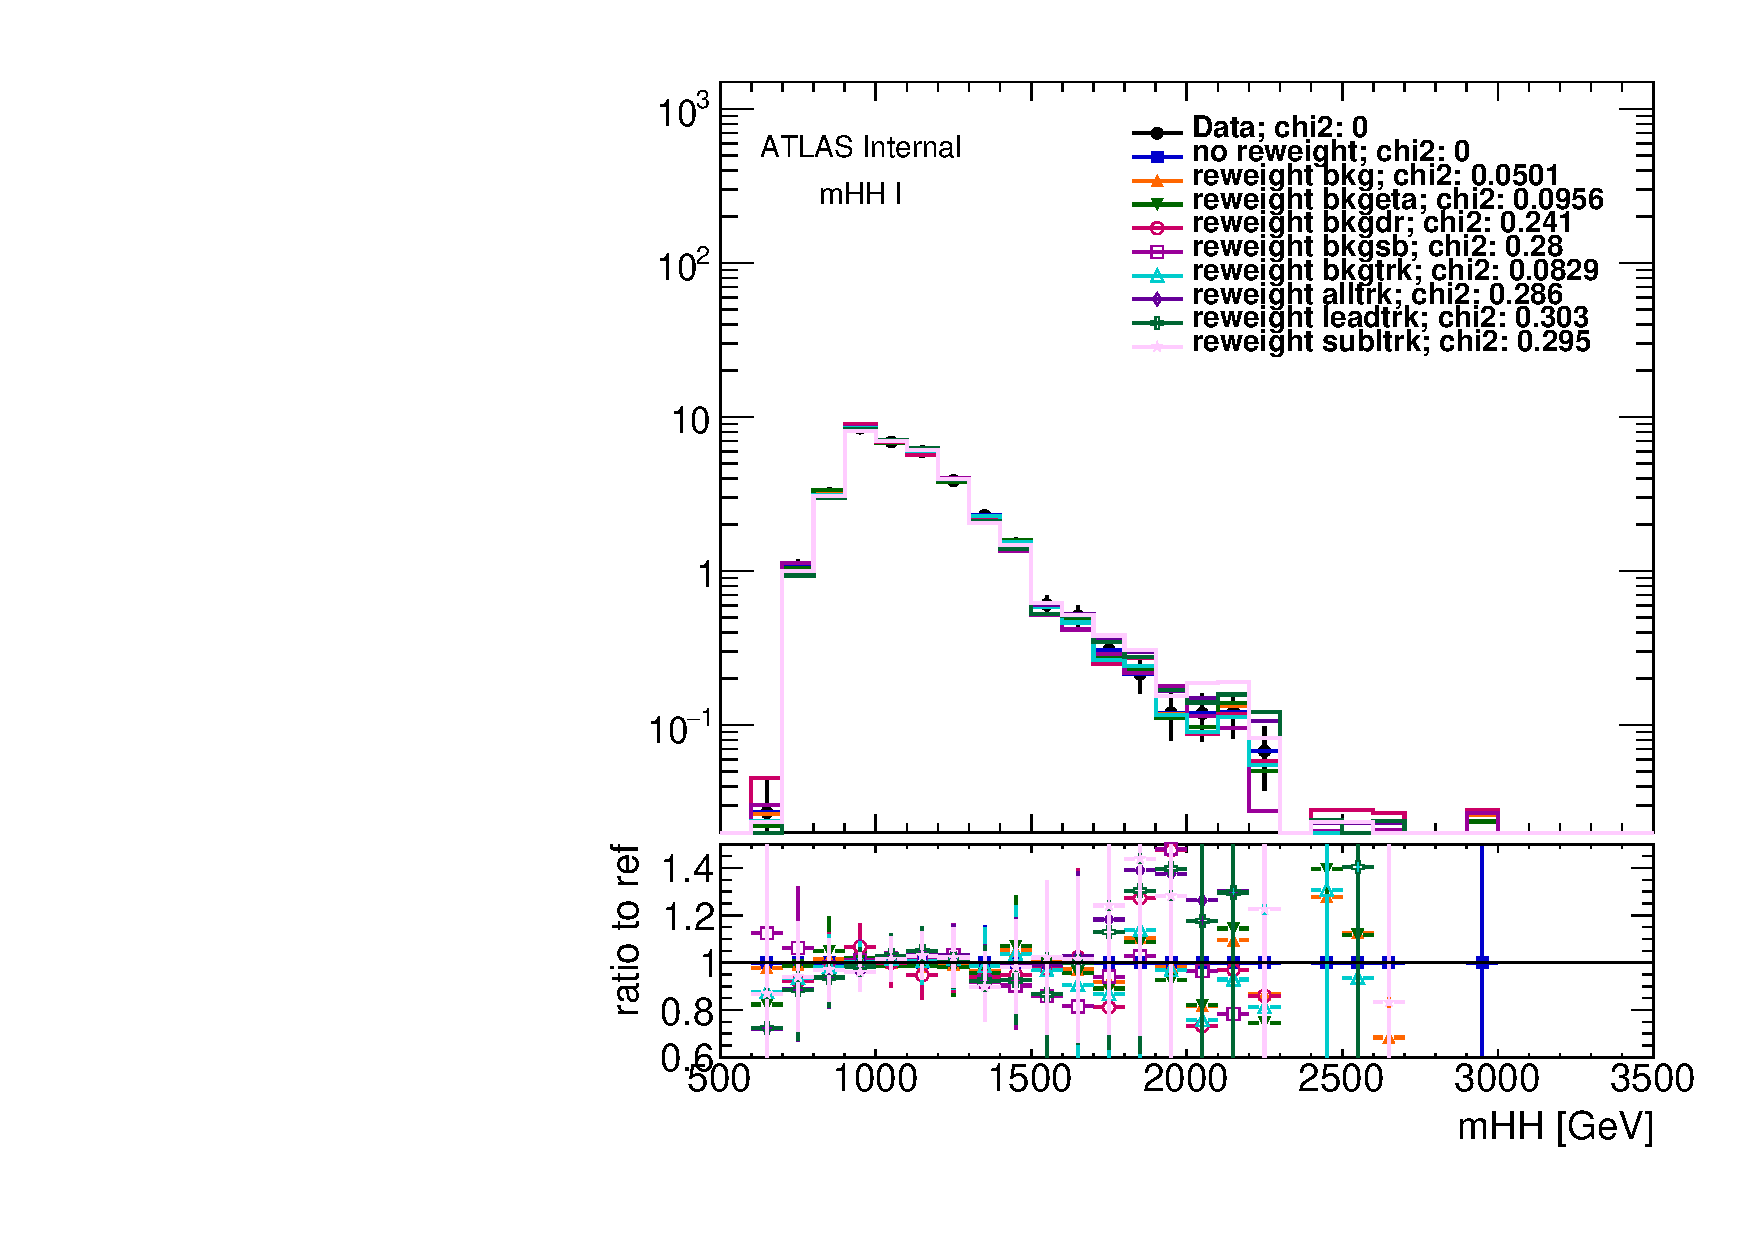
\includegraphics[width=0.4\textwidth,angle=-90]{figures/boosted/AppendixReweight/Compare/Data_FourTag_Signal_directcompare_mHH_l_1.pdf}
\caption{Reweighted $4b$ Sideband (top)/Control (middle)/Signal(bottom) region predictions comaprison, for MJJ. The Signal region is blinded, where the distribution is replaced with the non-reweighted distributions.}
\label{fig:app-rw-comp-4b}
\end{center}
\end{figure*}

\begin{figure*}[htbp!]
\begin{center}
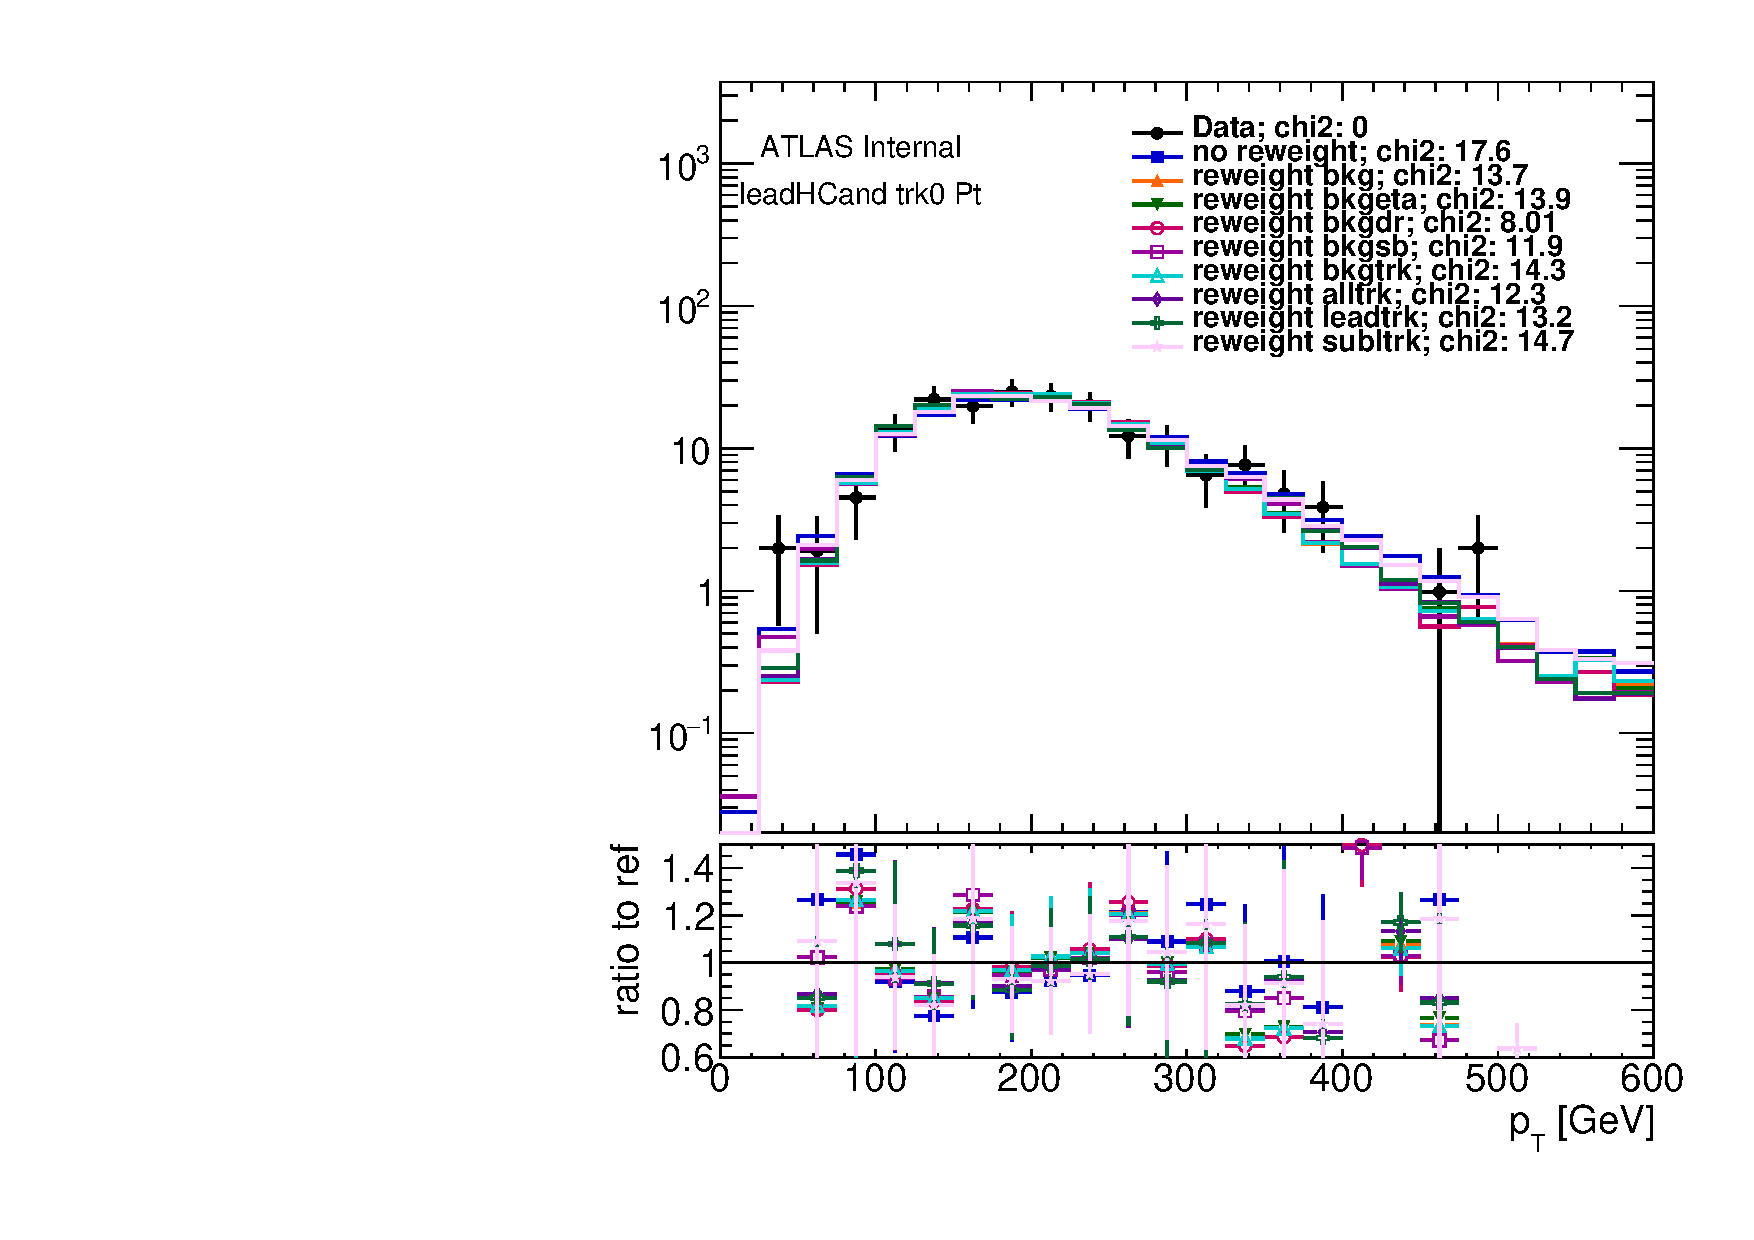
\includegraphics[width=0.24\textwidth,angle=-90]{figures/boosted/AppendixReweight/Compare/Data_FourTag_Sideband_directcompare_leadHCand_trk0_Pt_1.pdf}
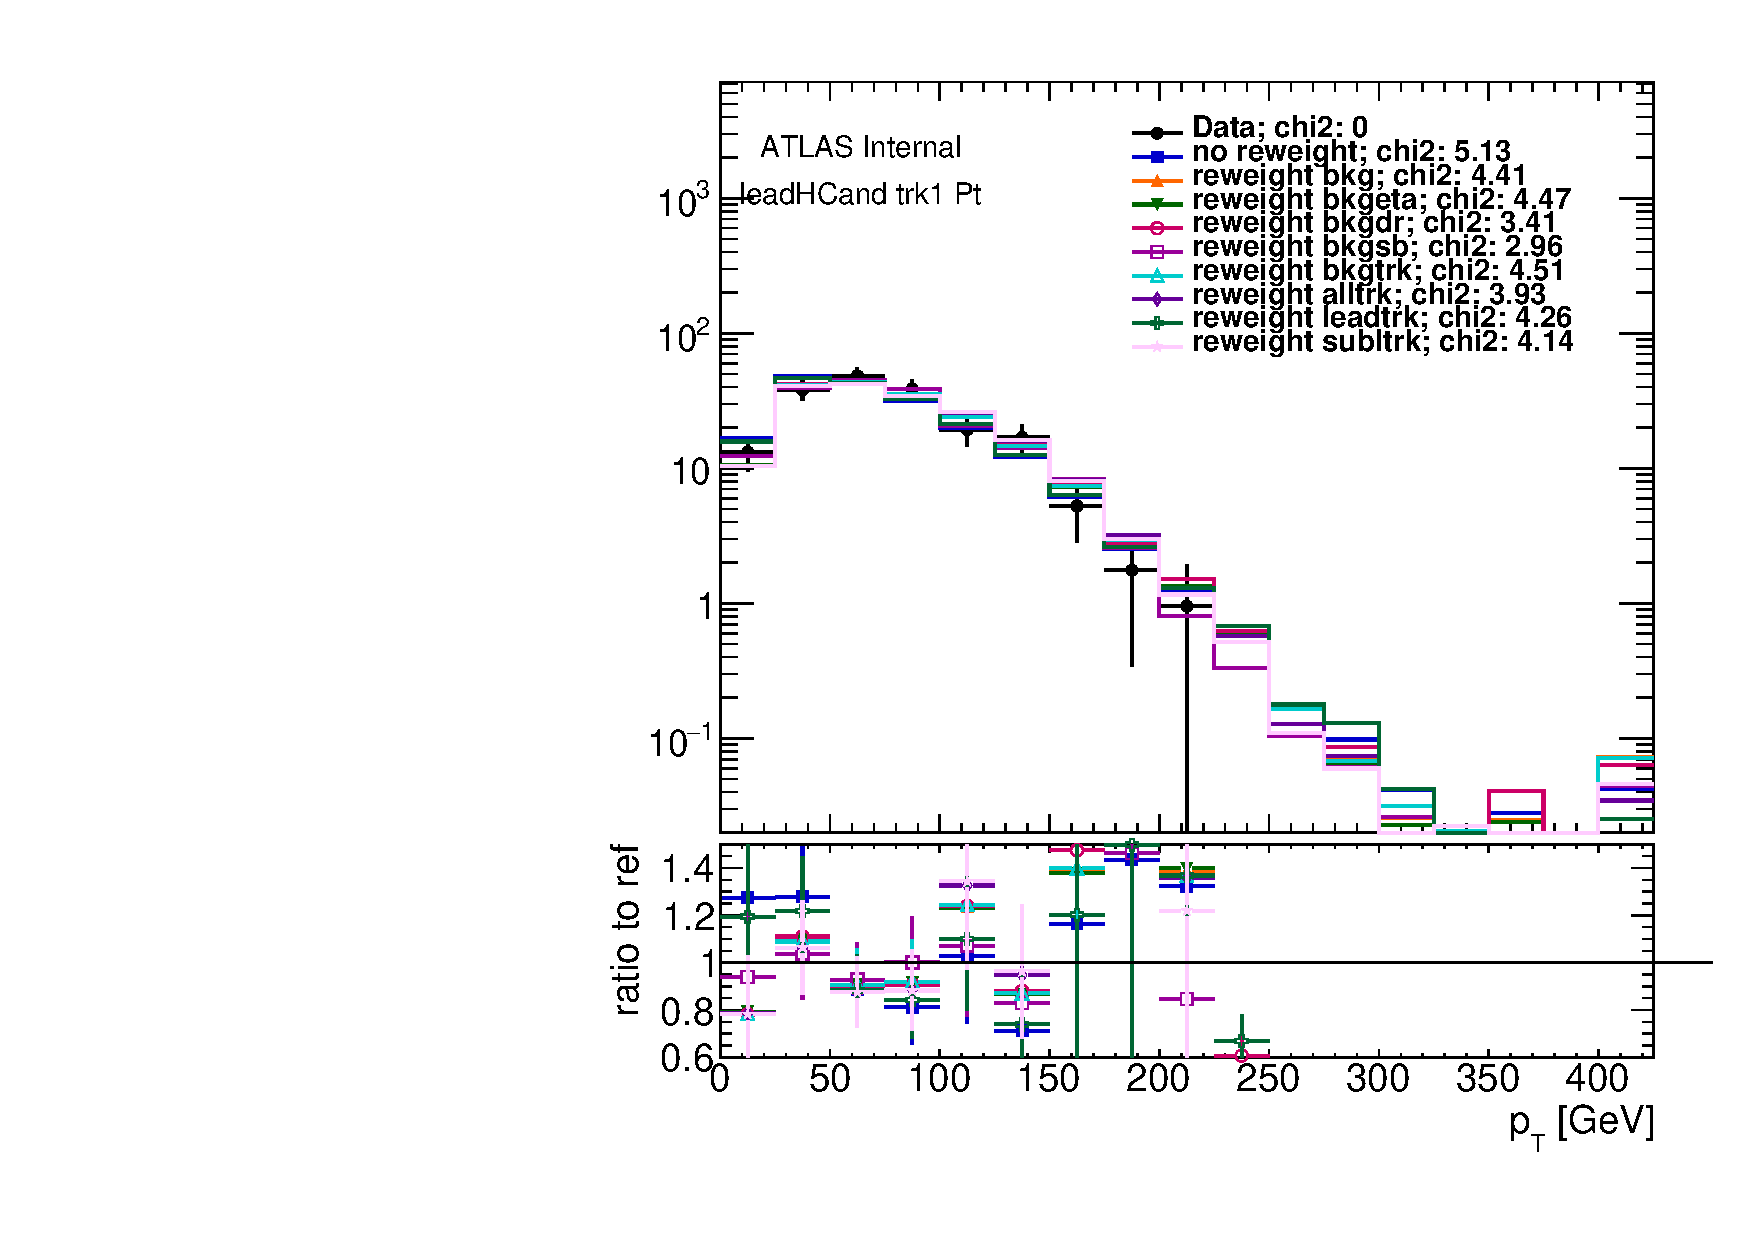
\includegraphics[width=0.24\textwidth,angle=-90]{figures/boosted/AppendixReweight/Compare/Data_FourTag_Sideband_directcompare_leadHCand_trk1_Pt_1.pdf}
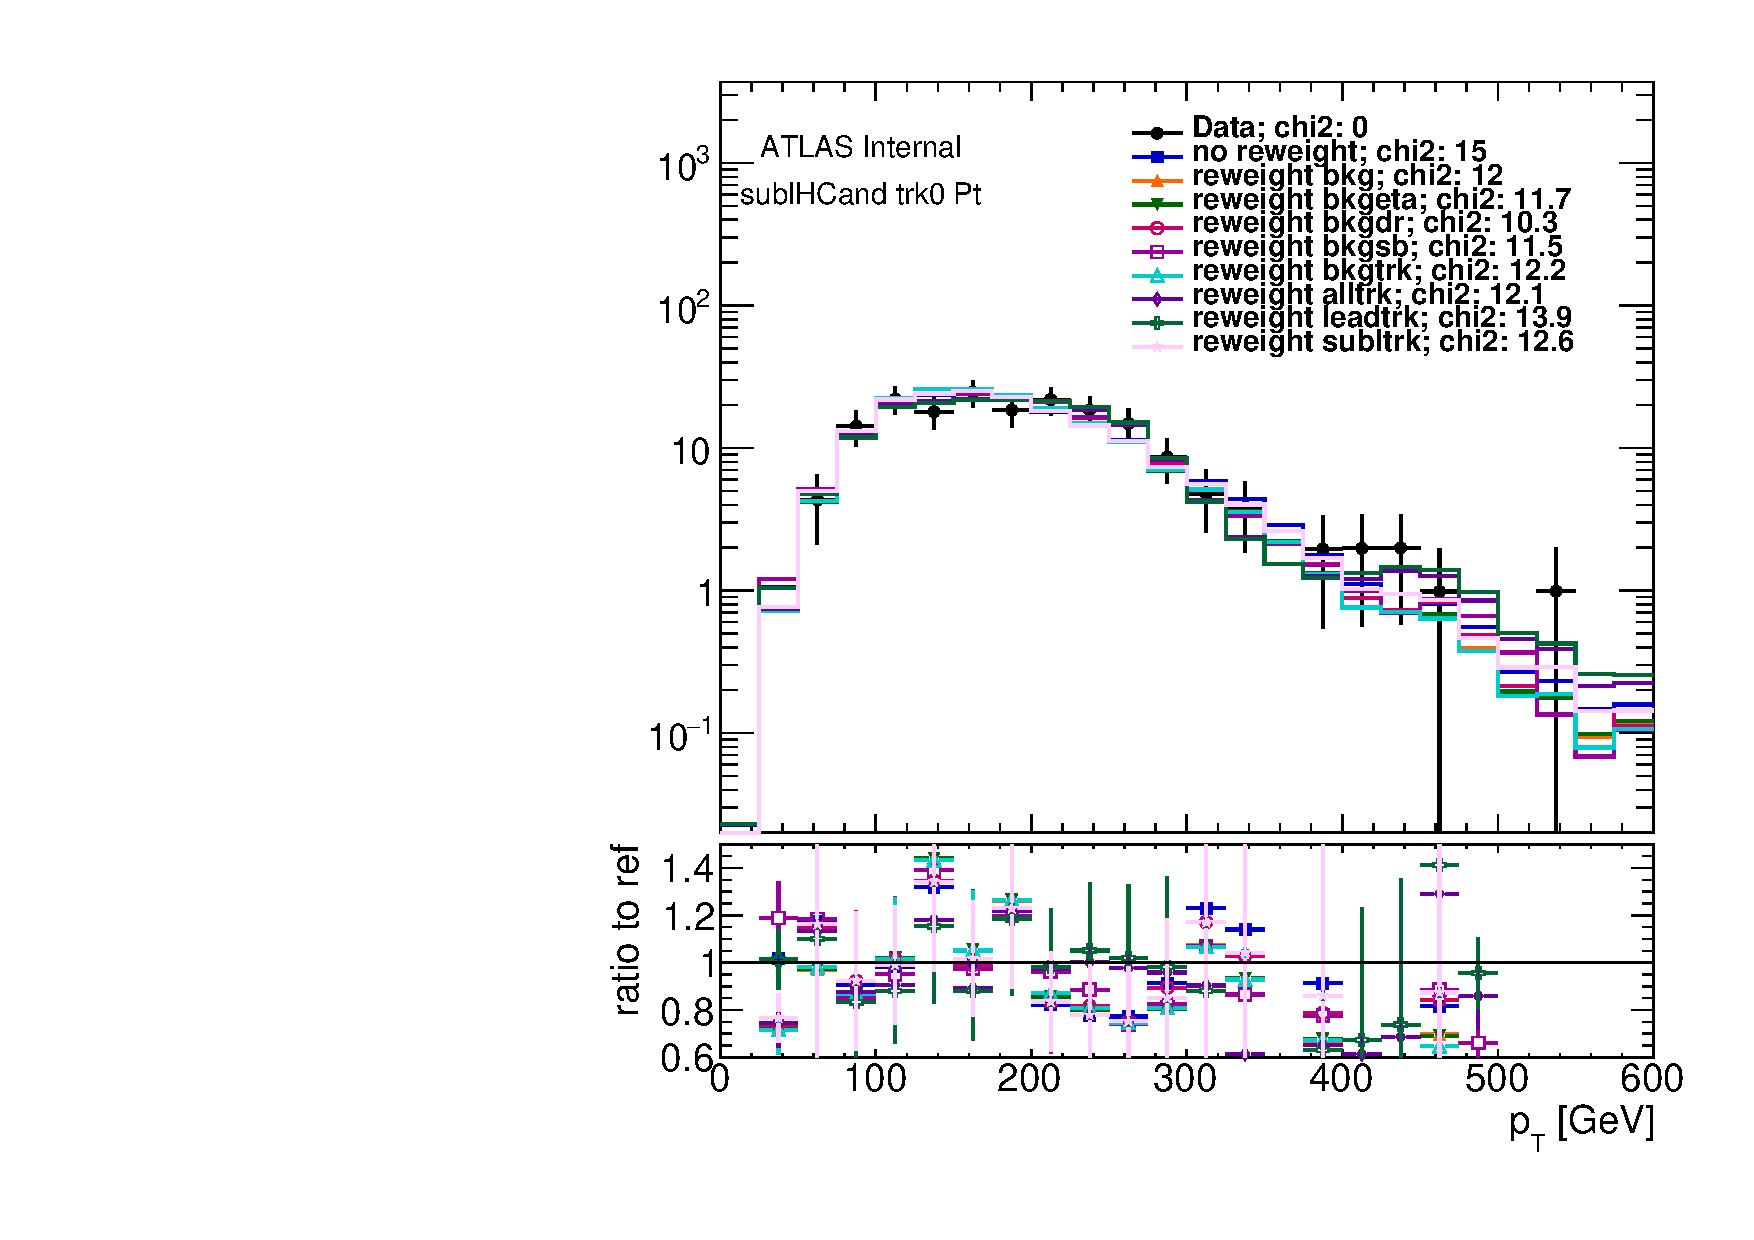
\includegraphics[width=0.24\textwidth,angle=-90]{figures/boosted/AppendixReweight/Compare/Data_FourTag_Sideband_directcompare_sublHCand_trk0_Pt_1.pdf}
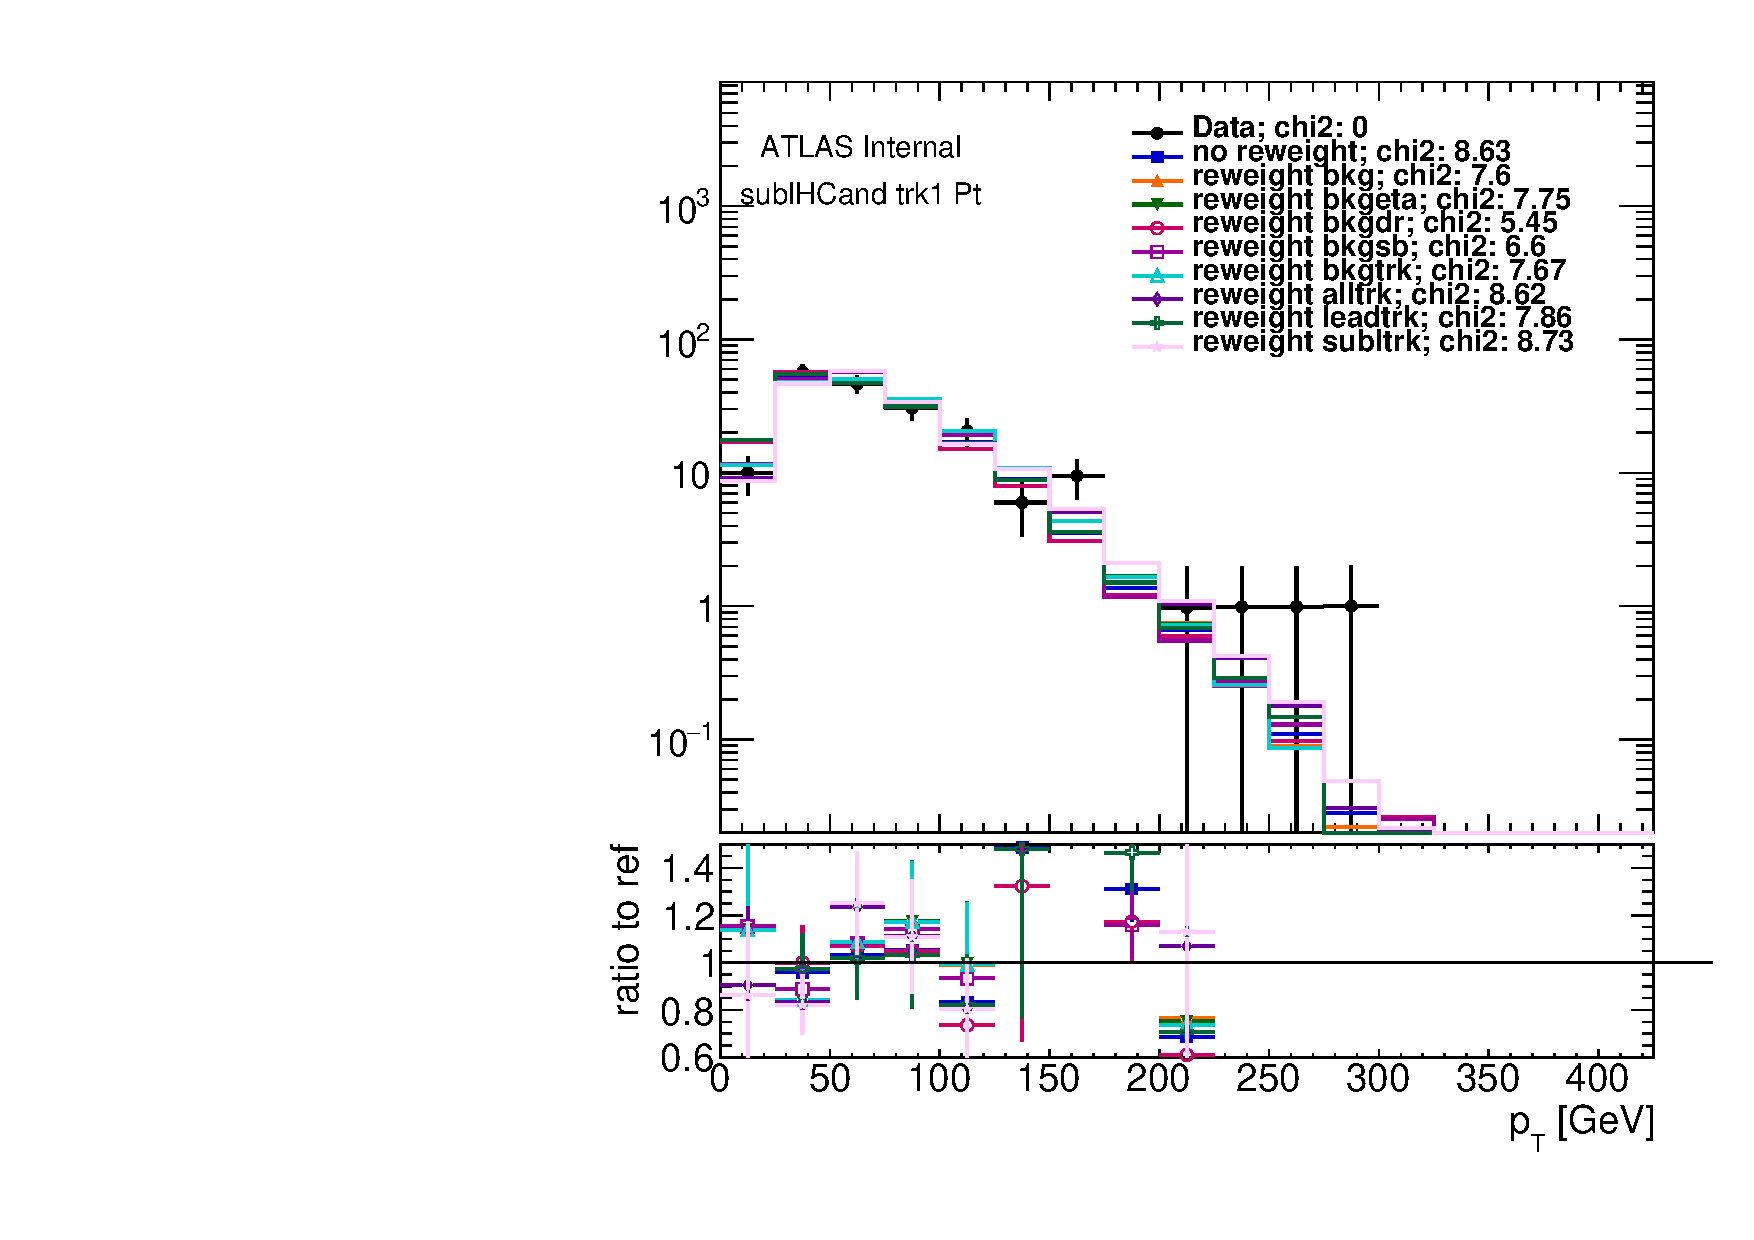
\includegraphics[width=0.24\textwidth,angle=-90]{figures/boosted/AppendixReweight/Compare/Data_FourTag_Sideband_directcompare_sublHCand_trk1_Pt_1.pdf}\\
\includegraphics[width=0.24\textwidth,angle=-90]{figures/boosted/AppendixReweight/Compare/Data_FourTag_Control_directcompare_leadHCand_trk0_Pt_1.pdf}
\includegraphics[width=0.24\textwidth,angle=-90]{figures/boosted/AppendixReweight/Compare/Data_FourTag_Control_directcompare_leadHCand_trk1_Pt_1.pdf}
\includegraphics[width=0.24\textwidth,angle=-90]{figures/boosted/AppendixReweight/Compare/Data_FourTag_Control_directcompare_sublHCand_trk0_Pt_1.pdf}
\includegraphics[width=0.24\textwidth,angle=-90]{figures/boosted/AppendixReweight/Compare/Data_FourTag_Control_directcompare_sublHCand_trk1_Pt_1.pdf}\\
\includegraphics[width=0.24\textwidth,angle=-90]{figures/boosted/AppendixReweight/Compare/Data_FourTag_Signal_directcompare_leadHCand_trk0_Pt_1.pdf}
\includegraphics[width=0.24\textwidth,angle=-90]{figures/boosted/AppendixReweight/Compare/Data_FourTag_Signal_directcompare_leadHCand_trk1_Pt_1.pdf}
\includegraphics[width=0.24\textwidth,angle=-90]{figures/boosted/AppendixReweight/Compare/Data_FourTag_Signal_directcompare_sublHCand_trk0_Pt_1.pdf}
\includegraphics[width=0.24\textwidth,angle=-90]{figures/boosted/AppendixReweight/Compare/Data_FourTag_Signal_directcompare_sublHCand_trk1_Pt_1.pdf}\\
\caption{Reweighted $4b$ Sideband (top)/Control (middle)/Signal(bottom) region predictions comaprison, for leading Higgs Candidate leading trackjet \pt (first column),  leading Higgs Candidate subleading trackjet \pt (second column), subleading Higgs Candidate leading trackjet \pt (third column), subleading Higgs Candidate subleading trackjet \pt (fourth column). The Signal region is blinded, where the distribution is replaced with the non-reweighted distributions.}
\label{fig:app-rw-comp-4b-trkjet}
\end{center}
\end{figure*}

\clearpage
